% CHAPITRE 3
\singlespacing
\chapter{Bilan de C de la tourbière de La Guette}
\label{ch:ch3}

\minitoc

\newpage
\doublespacing
\section{Introduction}
Les tourbières jouent un rôle important de stockage du carbone à l'échelle globale (cf chapitre~\ref{ch:ch1}).
En outre, ces écosystèmes ont une diversité importante que ce soit dans leur fonctionnement naturel ou les perturbations qu'elles subissent.
Cependant il existe peu d'estimations de leur bilan de carbone prenant en compte à la fois la contribution du \coo, du \chh et du COD.
%Elles ne sont d'ailleurs pas intégrées dans les modèles globaux 
La majorité des écosystèmes tourbeux pour lesquels un bilan de carbone a été estimé se situe sous les hautes latitudes de l'hémisphère nord comme en Suède \citep{waddington2000,peichl2014}, en Finlande \citep{Alm1997}, au Canada \citep{trudeau2014}.
Les estimations du bilan de carbone de tourbières situées plus au sud, notamment en Europe, sont plus rares (exemple d'une tourbière du Jura français, \citealp{bortoluzzi2006a}). 
De nombreuses études ont été faites sur les tourbières au Canada, mais le climat y est différent, avec des hivers plus froids pour des latitudes équivalentes.
%Les tourbières situées plus au sud ont fait l'objet de rare estimation de bilan (e.g. tourbière du Jura français par \citet{bortoluzzi2006a}).
L'étude de ces écosystèmes présents à la limite sud de leur extension est importante.
En effet, ils expérimentent des conditions plus extrêmes que les autres et qui, sans être identiques, peuvent se rapprocher de celles que subiront d'autres écosystèmes tourbeux suite au réchauffement climatique.

Plus spécifiquement le site d'étude, la tourbière de La Guette, est représentative d'une grande partie des tourbières vis-à-vis des perturbations qu'elle subie : drainage et envahissement par une végétation vasculaire (Les caractéristiques du site sont détaillées dans le chapitre~\ref{ch:ch2}).
On attend que cet envahissement se traduise par une aération du milieu plus importante, liée au développement des racines.
Cette aération favoriserais une RE élevée et un fonctionnement en source de carbone.

Le \textbf{premier objectif} de ce chapitre est donc d'\textbf{établir le bilan de C} de la tourbière de La Guette, afin de mieux comprendre comment fonctionne cet écosystème et de mettre en perspective ce fonctionnement par rapport aux tourbières des hautes latitudes.
% mais également comme il se situe par rapport à des écosystèmes établi dans des zones a priori plus favorables.
%L'intérêt est double, d'une part car ce site est représentatif d'une grande partie des tourbières dans les perturbations qu'elle subie : son drainage et son envahissement par une végétation vasculaire (cf Chapitre 2).
%D'autre part sa position en basse latitude la place dans des conditions environnementale qui, sans être identiques, peuvent se rapprocher de celles que subiront d'autres écosystèmes tourbeux suite au réchauffement climatique.

Le \textbf{second objectif} est de \textbf{caractériser la variabilité spatiale} de ces flux de GES à travers ce bilan de C.
En effet les tourbières sont des écosystèmes avec des conditions environnementales qui peuvent varier dans l'espace.
Par exemple le niveau de la nappe d'eau peut, à cause de variation micro-topographique, être plus ou moins élevé, immerger la surface du sol avec des zones d'eau libre ou au contraire être quelques dizaines de centimètres sous la surface du sol.
La conséquence de ces variations, est l'existence de micro-environnements différents qui abritent des communautés végétales et microbiennes différentes.
Finalement les variations des conditions environnementales contrôlant les flux, entraîne la variation des flux.
Estimer ces variations est donc nécessaire afin de préciser dans quelle mesure elles influent sur le bilan de C.

\section{Procédure expérimentale et analytique}

Cette partie contient la description de la stratégie d'échantillonnage et le détail des méthodes de mesure, les méthodes de chambre utilisées pour la mesure de flux de GES ont été détaillées dans la partie~\ref{sec:clsd_chbr_method}.
Elle explicite également le calcul de variables élaborées utilisées par la suite, détaille le principe permettant l'estimation du bilan de carbone du site à l'échelle saisonnière et décrit la stratégie d'étude de la variabilité spatiale.
Enfin elle précise comment sont calculées les erreurs associées aux flux et bilans.

\subsection{Design expérimental}

En juin 2011, 20 placettes ont été installées selon un échantillonnage aléatoire stratifié:
La surface de la tourbière active (\SI{13}{\hectare}) a été divisée selon une grille de 20 mailles et un point, choisi aléatoirement dans chaque maille, localise chaque placette (Figure~\ref{fig:carteVS}).
La taille de la maille a été ajustée de manière à avoir vingt 20 carrés sur la surface de la tourbière.
Cette méthode permet de conserver un échantillonnage aléatoire tout en ayant une représentativité spatiale homogène du site. 
Les placettes, délimitées par des piquets, occupent une surface de \SI{4}{\square\metre} (2$\times$\SI{2}{\metre}).
Usuellement, les placettes sont séparées en groupes micro-topographiques (Figure~\ref{fig:microtopo}), avec des embases positionnées sur les buttes (\textit{hummock}), les trous (\textit{hollows}) et les zones d'eau libre (\textit{pool}) \citep{Alm1997,waddington2000}.
Ou encore selon différent traitements, réhabilité/non réhabilité, exploité/non exploité, manipulé/non manipulé \citep{bortoluzzi2006a,strack2013}.
Cette méthodologie présente l'avantage de permettre une distinction fine des capacités sources/puits entre ces traitements.
Cependant elle implique généralement un placement des embases proches les unes des autres au sein d'un même traitement, limitant la représentativité spatiale des mesures.
%Ceci a l'avantage de permettre une distinction fine des capacités sources/puits mais a l'inconvénient du placement proche des embases les unes des autres limitant la représentativité spatiale des mesures.
%Elles peuvent également être séparées en zone dans la tourbière, haut-marais \textit{versus} bas-marais, ou réhabilité \textit{versus} non-réhabilité.
%Afin de gagner en représentativité spatiale, la taille du site le permettant, il a donc été décidé de positionner des placettes sur l'ensemble du site.
Le placement des 20 embases sur l'ensemble de site, sa taille l'autorisant, permet de gagner en représentativité spatiale.
Sur ces placettes ont été réalisées des mesures de \textbf{flux de gaz} et de \textbf{facteurs contrôlant}.

\begin{figure}
\centering
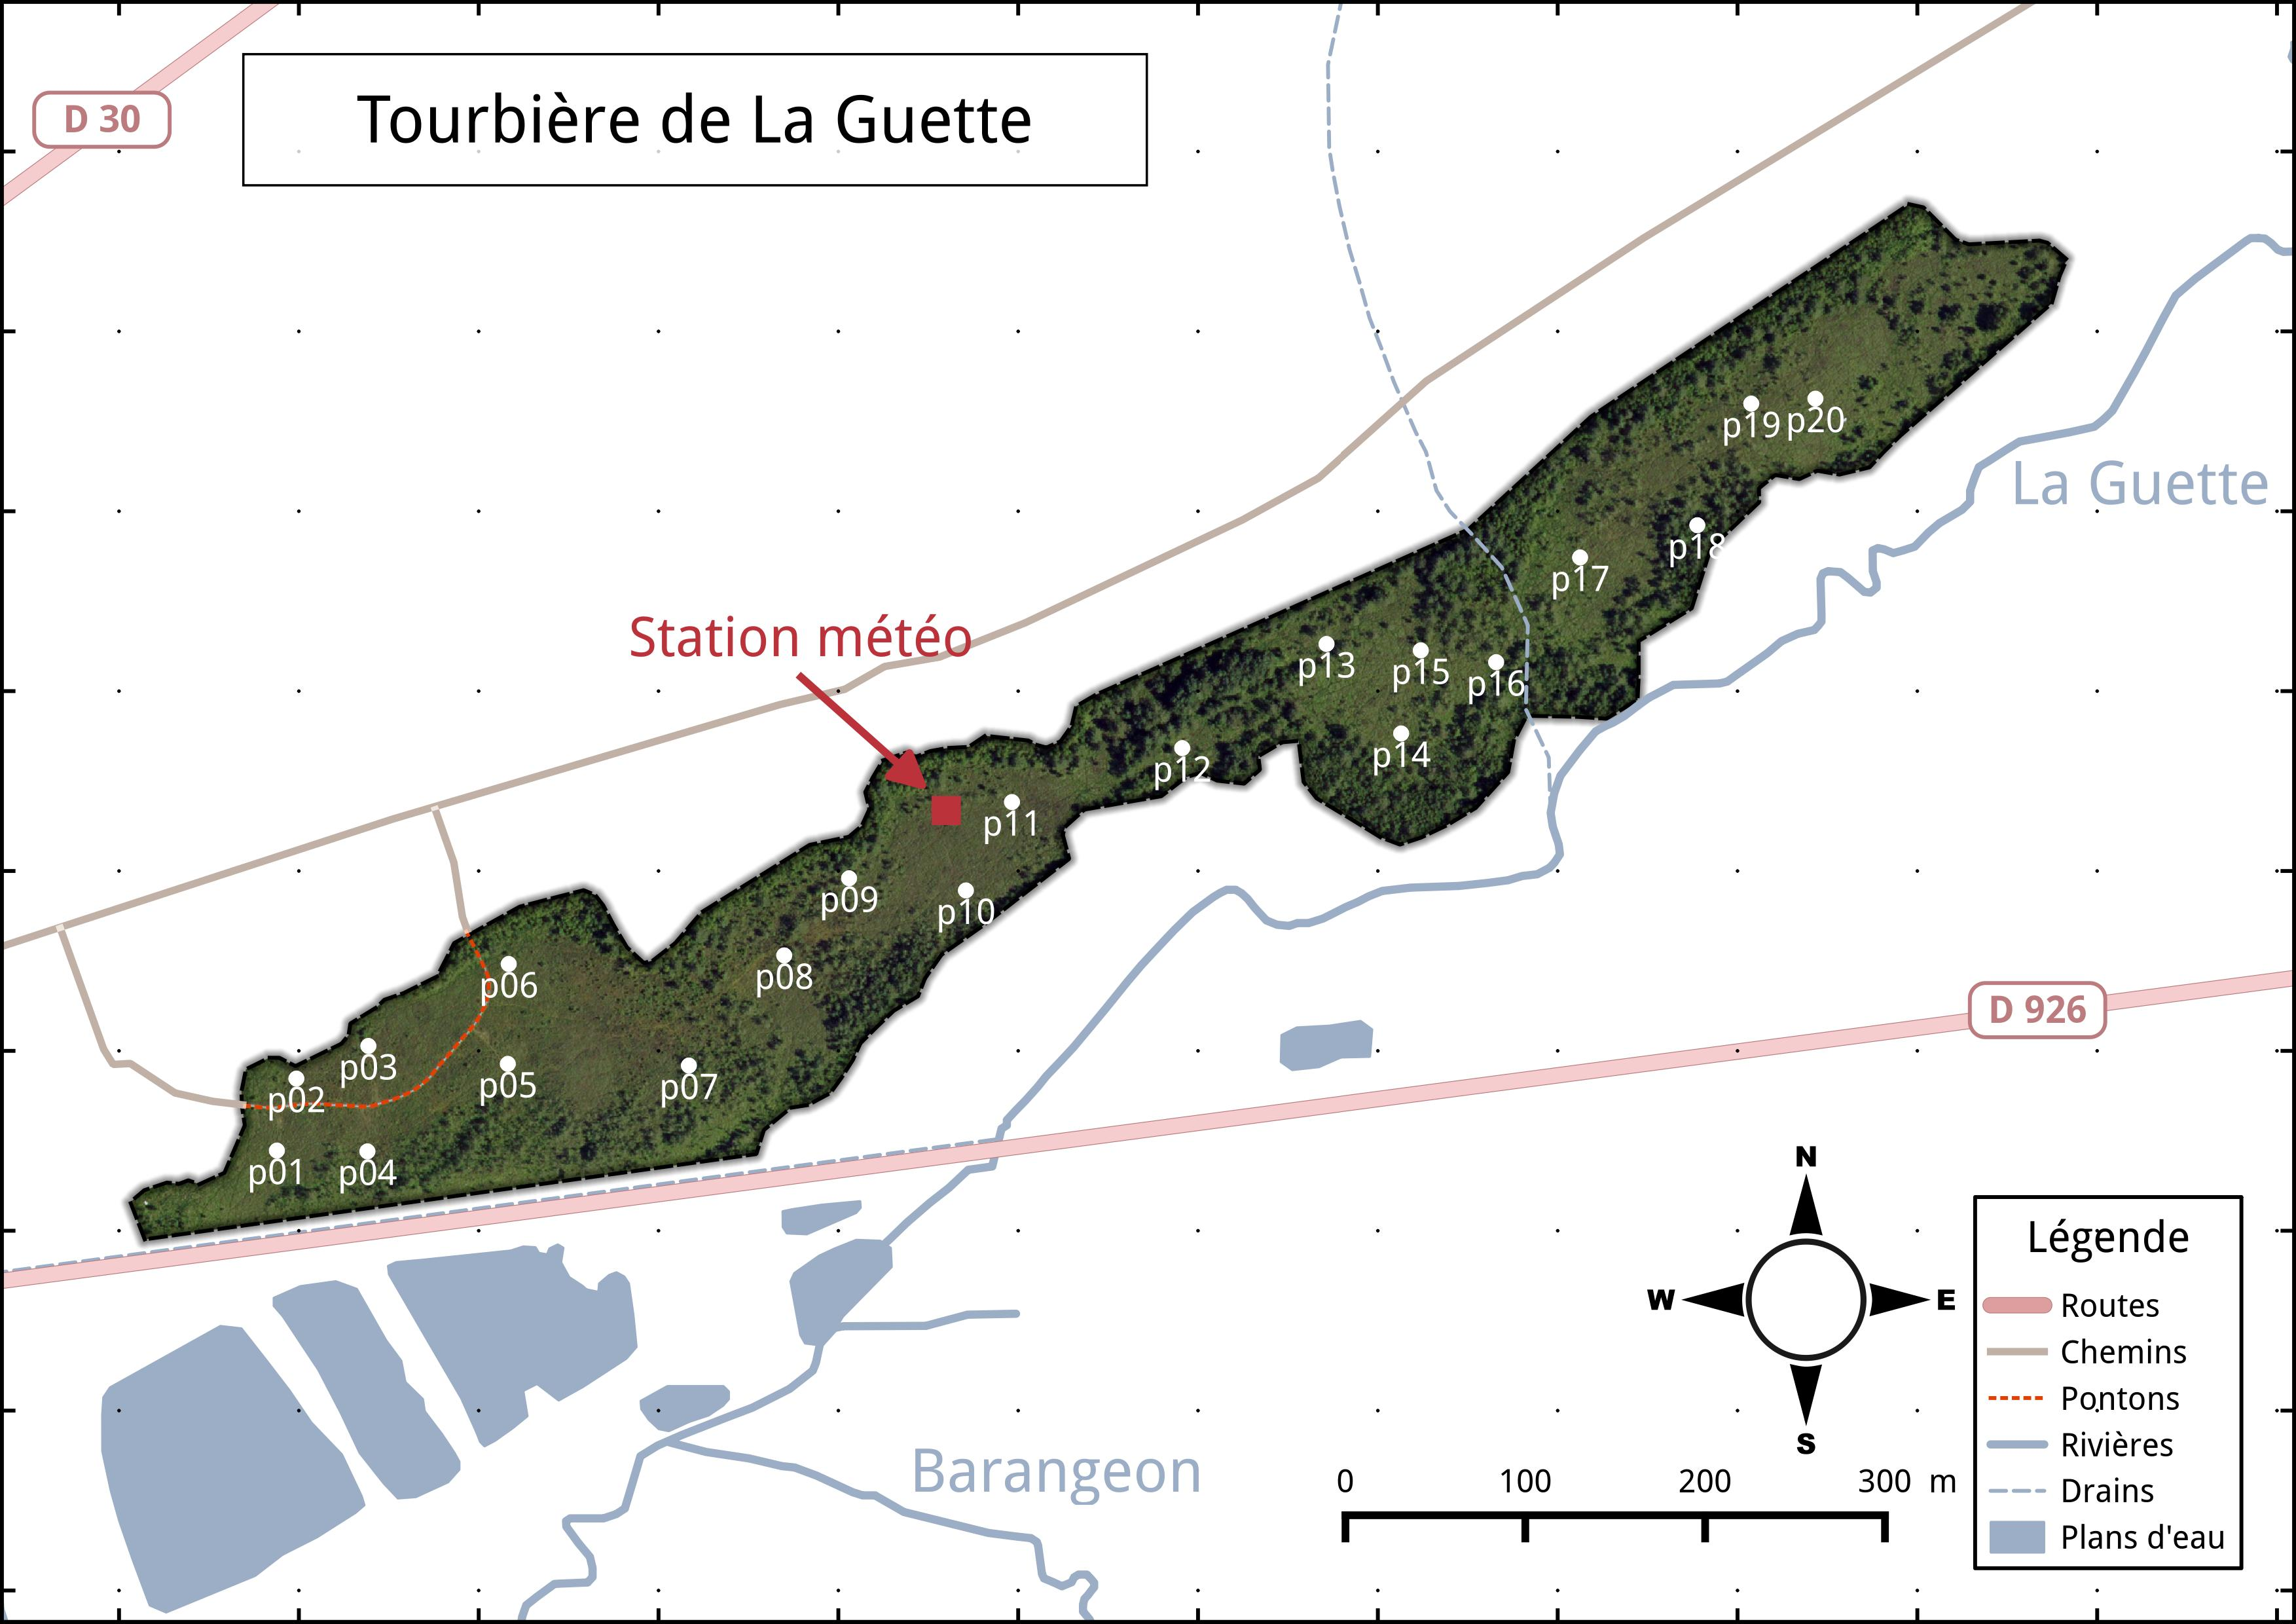
\includegraphics[width=\textwidth]{chap3/carteVS}
\caption{Répartition des 20 placettes de mesures suivant un échantillonnage aléatoire stratifié.}
\label{fig:carteVS}
\end{figure}

\subsubsection{Mesures des flux de gaz}

Les mesures des flux de \coo et de \chh ont été effectuées en utilisant les méthodes de chambre décrites dans la partie~\ref{sec:clsd_chbr_method}.
À l'intérieur de chaque placette ont été installé de façon permanente un piézomètre et une embase permettant la mesure des flux de gaz (Les embases sont décrites dans le chapitre~\ref{ch:ch2}, partie~\ref{subsec:ss_mes_co2}).

%De plus, du fait de l'omniprésence de végétation vasculaire, et de la taille des chambres par rapport à la micro-topographie une telle approche était difficile à mettre en oeuvre.

Initialement, les flux de \coo, \chh et N\textsubscript{2}O devaient être mesurés et étudiés (Tableau~\ref{table:ls_var}).
Cependant, suite à des tests préliminaires effectués sur la tourbière montrant des émissions très faibles de N$_{2}$O, ce gaz n'a pas été étudié.
Les mesures de \coo ont été effectuées de mars 2013 à février 2015, avec une fréquence quasiment mensuelle (20 campagnes, pour 24 mois de mesures, sur les 20 placettes). 
Chaque campagne de mesure s'étend sur deux journées et nécessite la présence de deux personnes afin de pouvoir mesurer l'ensemble des 20 placettes.
Les mesures de \chh ont été effectuées avec une fréquence et sur un nombre d'embases inférieur (12 campagnes, 5 embases).
Ceci a été déterminé par la difficulté de déploiement \textit{in-situ} de l'instrument SPIRIT : il est lourd, difficilement transportable dans un milieu tourbeux et nécessite entre chaque déplacement un temps de mise en marche/arrêt important (plus de \SI{30}{\minute}).
Les mesures se sont donc limitées aux placettes accessibles depuis le ponton (placette n°1 à 6, figure~\ref{fig:carteVS}).

% (lourd, difficilement transportable dans un milieu tourbeux).

\subsubsection{Mesures du COD}

Des échantillons d'eau prélevés à l'exutoire de la tourbière ont été prélevés, et leur concentration en COD a été mesurée moins de 24 heures après le prélèvement.
Les analyses de COD ont été faite, après filtration à \SI{0.45}{\micro\metre} en utilisant la technique dite NPOC (\textit{Non Purgeable Organic Carbon}) dans laquelle le carbone inorganique présent dans l'échantillon est transformé en \coo par l'ajout d'un acide puis évacué (purgé) avant que l'échantillon ne soit injecté dans un four et analysé par un détecteur Infra-rouge.

\subsubsection{Mesures des facteurs contrôlant}


\begin{table}
\centering
\caption{Liste des variables acquises. Les données acquises manuellement sont réalisées sur les 20 placettes, tandis que les données acquises automatiquement sont réalisées par la station météorologique (1 seul point).}
\label{table:ls_var}
\begin{tabular}{llll}
\toprule
& variable & type d'acquisition & fréquence \\
\midrule
\multicolumn{4}{l}{Flux} \\ [+.5ex]
& \coo & manuelle & mensuelle \\
& \chh & manuelle & mensuelle \\[+1ex]
\multicolumn{4}{l}{Physique} \\ [+.5ex]
& rayonnement photosynthétique actif & manuelle & mensuelle \\
& température air & manuelle & mensuelle \\
& température sol & manuelle & mensuelle \\
& température air & automatique & horaire \\
& température sol & automatique & horaire \\[+1ex]
\multicolumn{4}{l}{Hydrologie} \\ [+.5ex]
& niveau de nappe & manuelle & mensuelle \\
& niveau de nappe & automatique & horaire \\
& conductivité & manuelle & mensuelle \\
& pH & manuelle & mensuelle \\
& COD & manuelle & mensuelle \\
& teneur en eau & manuelle & mensuelle \\[+1ex]
\multicolumn{4}{l}{Végétation} \\ [+.5ex]
& pourcentage de recouvrement végétal & manuelle & mensuelle \\[+1ex]
\multicolumn{4}{l}{Météorologie} \\ [+.5ex]
& pluviométrie & automatique & horaire \\
& pression atmosphérique & automatique & horaire \\
& humidité de l'air & automatique & horaire \\
& rayonnement solaire & automatique & horaire \\
& vent (vitesse et direction) & automatique & horaire \\
\bottomrule
\end{tabular}
\end{table}


Les facteurs contrôlant mesurés manuellement sont la pression atmosphérique, le rayonnement photosynthétique actif (\textit{photosyntheticaly active radiation}, PAR), les températures du sol à différentes profondeurs, la végétation (pourcentage de recouvrement), le niveau de la nappe d'eau (Tableau~\ref{table:ls_var}).
La pression atmosphérique est mesurée au début et à la fin des mesures de flux.
Le PAR est mesuré au début et à la fin des mesures de l'ENE.
Le recouvrement de végétation est estimé visuellement.
Des prélèvements d'eau ont été effectués chaque mois pour mesurer le pH et la conductivité (mesures effectuées sur le terrain après les mesures de flux).
Les échantillons d'eau prélevés dans les 20 placettes ont été congelés pour la mesure ultérieure de la concentration en carbone organique dissout (COD).
Dans les tourbières la quantité de carbone inorganique est généralement considéré comme négligeable \citep{worrall2009}.

L'ensemble de ces mesures nécessitant d'accéder aux placettes régulièrement, des planches de bois ont été utilisées comme pontons mobiles pour limiter les perturbations. La dispersion des placettes sur l'ensemble du site a rendu impossible une installation plus permanente.

Les mesures automatiquement acquises via la station météo installée sur le site depuis 2010 sont la température de l'air, la température de la tourbe à \num{-5}, \num{-10}, \num{-20} et \SI{-40}{\centi\metre} de profondeur, la vitesse et la direction du vent, l'humidité relative de l'air, le rayonnement solaire, et la pression atmosphérique (Tableau~\ref{table:ls_var}).

\subsection{Variables élaborées utilisées}

Les mesures de recouvrement de la végétation ont été sommées par strate végétale.
On utilisera donc RSM, RSH, RSA pour distinguer les recouvrements respectif de la strate muscinale (\textit{Sphagnum spp.}), herbacée (\textit{Molinia caerula} et \textit{Eriophorum augustifolium}) et arbustive (\textit{Erica tetralix} et \textit{Calluna vulgaris}).
Un indice de végétation, représentant la quantité de végétation présente dans une embase est également calculé de la façon suivante : 

\begin{equation}
IV = \frac{RSM + RSA + RSH}{\sum R{max}}
\end{equation}

Avec :
\begin{itemize}
\item $\sum R_{max}$ La somme des pourcentage de recouvrements maximum par strates.
\item RSM le pourcentage de recouvrement de la strate muscinale mesuré
\item RSH le pourcentage de recouvrement le la strate herbacée mesuré
\item RSA le pourcentage de recouvrement de la strate arbustive mesuré
\end{itemize}

Le niveau de nappe est composé de deux mesures, l'une du haut du piézomètre jusqu'au niveau de la nappe et l'autre du haut du pièzomètre jusqu'à la surface du sol. 
Par la suite, et en l'absence de précisions, le niveau de nappe se réfère à la différence entre ces deux mesures et donc à la distance entre la surface du sol et le niveau de la nappe (Négative sous la surface du sol et inversement).
En cas de présence de Sphaignes, le haut des capitulums est pris comme référence (z=0)

\subsection{Estimation des flux de GES dans le bilan de C}

L'estimation des flux de GES pour calculer un bilan de carbone se fait en trois étapes.
La première consiste à établir des relations empiriques entre les flux et un ou plusieurs facteurs contrôlant.
C'est la phase de \textbf{calibration}.
La seconde, l'\textbf{évaluation}, teste la pertinence de ces relations sur un jeu de données indépendantes.
La troisième, l'\textbf{interpolation}, utilise ces relations empiriques et les données acquises à plus haute fréquence, pour intégrer dans le temps les mesures ponctuelles sur l'ensemble des deux années de mesure. 
La chronique ainsi reconstituée permet ensuite d'estimer les quantités de carbone annuelles déplacées via des différents flux et d'en calculer leur bilan.

%\subsubsection{Estimation du bilan et variabilité temporelle}
\subsubsection{Calibration}

Pour estimer le bilan de carbone du site il est donc nécessaire d'établir des modèles reliant des flux mesurés ponctuellement avec des variables explicatives mesurées à haute fréquence (par exemple entre la respiration de l'écosystème et la température de l'air).
%Ces relations empiriques permettront d'interpoler les données acquises mensuellement sur l'ensemble des deux années de mesure et de reconstituer ainsi une chronique de flux dont l'intégration dans le temps permettra d'estimer une quantité de carbone sur l'année.
Pour établir ces modèles empiriques les données acquises ont été moyennées par campagne de mesure ; ceci permettant, dans un premier temps, de s'affranchir de la variabilité spatiale des flux et ne considérer que la variabilité temporelle.
Les relations entre flux et facteurs contrôlant ont ensuite été étudiées deux à deux, notamment en réalisant une analyse en composante principale (ACP).
Cette analyse permet de déterminer quels sont les relations entre les variables et plus particulièrement quelles sont celles qui détermine le plus les flux de GES.
Le nombre de données acquises pour le \coo et le \chh étant différent, une ACP a été réalisée pour chacun de ses gaz (Annexe~\ref{sec:acp}).
Une fois le facteur de contrôle prépondérant d'un gaz établi, grâce à l'ACP et à la littérature, une relation empirique est établie entre les deux.
%La forme de cette relation et la littérature conditionne ensuite les équations testées.
Elles sont évaluées à l'aide du coefficient de détermination (R\textsuperscript{2}) et de la racine carré de l'erreur quadratique normalisée par la moyenne (\textit{Normalised Root Mean Square Error}, NRMSE).
Le R$^{2}$ est utilisé comme indicateur de la proportion de la variabilité des données expliquée par le modèle, sa valeur est comprise entre 0 et 1 (pour les équations linéaires) : 

$$ R^{2} = 1 - \frac{\sum(y-\hat{y})^2}{\sum(y-\bar{y})^2} $$ 

Avec : 
\begin{itemize}
\item $y$ : données mesurées
\item $\hat{y}$ : données modélisées
\item $\bar{y}$ : la moyenne des données mesurées
\end{itemize}

La RMSE et sa normalisation par la moyenne NRMSE sont utilisés comme indicateur de l'écart entre les données mesurées et les données modélisées :

$$ RMSE = \sqrt{\frac{\sum(y - \hat{y})^2}{N}} $$

$$ NRMSE = 100 \times \frac{RMSE}{\bar{y}} $$

Avec les notations précédentes et : 
\begin{itemize}
\item $N$ : le nombre d'observations
%\item $\bar{y}$ : la moyenne des données mesurées
\end{itemize}
Les résidus\footnote{Les résidus sont défini comme la différence entre les valeurs mesurées et celles calculées par un modèle.} sont également étudiés dans le but d'éviter un biais ou une hétéroscédasticité\footnote{On parle d'homoscédasticité lorsque la variance de l'erreur d'une variable est constante, et l'hétéroscédasticité lorsque qu'elle ne l'est pas} dans les données (Figure~\ref{fig:ref_resid}).

\begin{figure}[!htb]
\centering
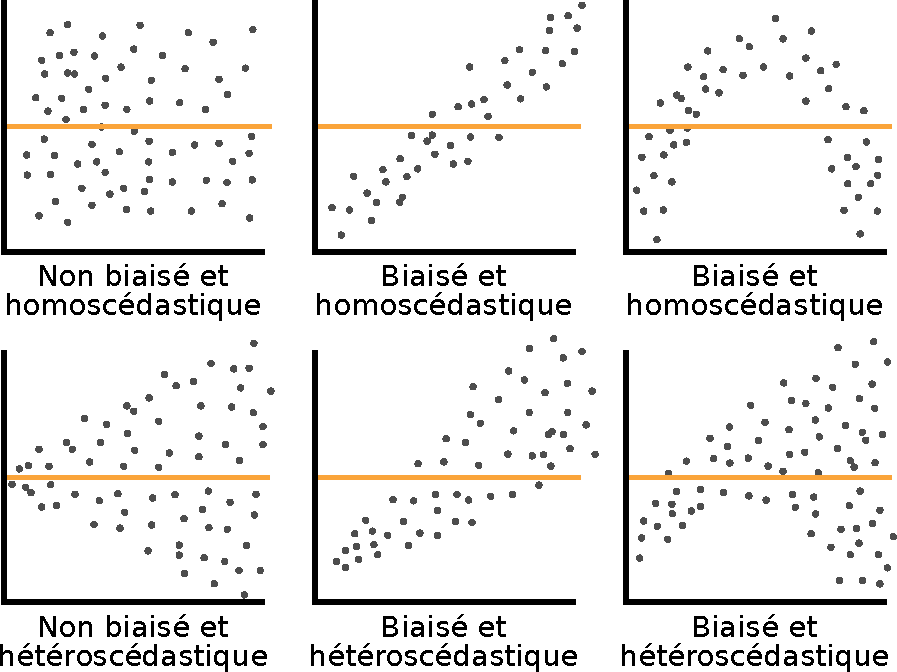
\includegraphics[width=\textwidth]{chap3/ref_resid}
\caption{Cas idéaux de distribution des résidus. Modifié d'après source inconnue, repris de : \url{https://danieljhocking.wordpress.com/2011/07/18/model-validation-interpreting-residual-plots/}}
\label{fig:ref_resid}
\end{figure}

Puis les résidus de ces modèles de base ont été étudiés en fonction des facteurs de contrôle restant.
Dans le cas où une tendance est visible avec l'un d'entre eux, le facteur est ajouté \citep{bortoluzzi2006a}.
En plus des indicateurs précédent, la pertinence de l'ajout d'un paramètre est évalué à l'aide du  critère d'information d'Akaike (\textit{Akaike Information Criterion}, AIC) \citep{akaike1974,burnham2002} :

$$ AIC = -2 \times log(L) + 2\times k $$ 

Avec :
\begin{itemize}
\item $L$ : le maximum de la fonction de vraisemblance
\item $k$ : le nombre de paramètres à estimer
\item $\bar{y}$ : la moyenne des données mesurées
\end{itemize}

L'AIC est un indicateur qui permet de déterminer si l'ajout d'un paramètre dans un modèle est pertinent (autrement dit, si l'ajout d'un paramètre vaut l'information qu'il apporte), afin d'éviter de le sur-ajuster.
Pour cela on considère la valeur la plus faible de l'AIC comme le meilleur indicateur.

%\vspace{\abovedisplayskip}

% \vspace{\belowdisplayskip}
 
%Les flux de \coo ont été modélisé en partant de l'équation ENE = PPB - RE, et le bilan a été établi en estimant de façon séparée la PPB et la RE.
%Cette séparation permettant de distinguer si une variation du bilan est liée à l'un ou l'autre des flux ou bien aux deux.
%Les flux en phase gazeuse ont été modélisés en partant d'équations usuellement utilisées et dans lesquelles la température est le facteur contrôlant majeur.
%Puis les résidus\footnote{Valeurs moyennes - Valeurs moyennes estimées} de ces modèles de base ont ensuite été étudiés en fonction des facteurs de contrôle restant.
%Dans le cas où une tendance est visible, le facteur est intégré.

%Les modèles ont été comparés avec différents indicateurs : Le coefficient de détermination (R\textsuperscript{2}), l'erreur standard normalisée (\textit{Normalised Root Mean Square Error}, NRMSE) et le critère d'information d'Akaike (\textit{Akaike Information Criterion}, AIC).
%Le R$^{2}$ est utilisé comme indicateur de la proportion de la variabilité des données expliquée par le modèle, sa valeur est comprise entre 0 et 1.
%La RMSE et sa normalisation par la moyenne NRMSE sont utilisés comme indicateur de l'écart entre les données mesurées et les données modélisées.
%L'AIC permet de déterminer la pertinence de l'ajout d'un paramètre sur la représentation des données par le modèle.

La température a été choisie comme base de départ à la construction des modèles de RE et PPB, car (i) c'est le facteur de contrôle le plus souvent invoqué dans la littérature et (ii) les corrélations avec les flux étaient les plus forte (cf ACP, annexe~\ref{sec:acp}).

\begin{center}
\begin{minipage}{.85\textwidth}
\setlength{\parindent}{-10pt}%
%\singlespacing
\onehalfspacing
\textbf{Remarque :} La RE, et l'ENE sont des flux mesurés directement sur le terrain à l'inverse de la PPB.
Cette dernière est déduite des deux flux précédents en utilisant l'équation $PPB = ENE - RE$.
Elle sera néanmoins appelée PPB mesurée, par opposition aux flux modélisés.
Afin d'établir le bilan de carbone tout en gardant une discrimination entre les flux entrants et sortants de l'écosystème la RE et la PPB ont été estimés séparément.
\end{minipage}
\end{center}

Concernant la respiration de l'écosystème, les températures utilisées dans la littérature sont variables.
La température la plus utilisée est la température du sol à \SI{-5}{\centi\metre}  \citep{ballantyne2014}.
D'autres auteurs utilisent aussi la température de l'air et la température du sol à \SI{-10}{\centi\metre} \citep{bortoluzzi2006a,kim1992}.
L'utilisation de ces profondeurs sont justifiées par le fait que dans la tourbe, la respiration du sol est la plus importante au dessus du niveau de l'eau et donc en surface \citep{Luo200661}. %\textbf{production CO2 ? profils ?}
C'est également en surface que se situent la majorité des racines \citep{rydin2013c}.
La respiration des racines contribue à la respiration de l'écosystème pour 35 à \SI{60}{\percent} \citep{silvola1996,crow2005}.
%La RE est estimée directement à partir des données acquises moyennées en partant de la température connue pour contrôler une grande partie de ce flux.
%Les modèles les plus fréquemment utilisés (linéaire, exponentiel, arrhénius) ont été testés.

Il ne semble pas émerger de consensus dans la littérature quant aux facteurs contrôlant les émissions de \chh.
Différents facteurs sont utilisés comme la température, \citep{alm1999,bubier1995b}, le niveau de la nappe \citep{bubier1993} ou encore la végétation \citep{bortoluzzi2006a}.
Ces facteurs peuvent être utilisés seuls ou conjointement.

\subsubsection{Évaluation/validation}

Après la phase de calibration, les facteurs de contrôle utilisés dans les modèles ont été évalués à l'aide de données indépendantes acquises en 2014, dans le cadre d'un suivi expérimental mis en place sur la tourbière de La Guette pour le projet CARBIODIV (cf annexe~\ref{sec:carbiodiv}).
%Cette dernière est également un suivi des mêmes flux de gaz, sur le même site pendant l'année 2014.
Les méthodes de mesures des flux de \coo et de \chh sont strictement identiques (ainsi que les opérateurs) à celles utilisées pour établir le bilan de carbone.
En revanche le positionnement des placettes est beaucoup plus classique : proches les unes des autres, et avec différents traitements.
Afin de pouvoir les comparer, seule les placettes de contrôles, (n'ayant donc subie aucune manipulation) de cette expérimentation seront utilisées soit 4 placettes dans une station en amont et 4 en aval de la tourbière de La Guette (plus de détails dans l'annexe~\ref{sec:carbiodiv}).
Le terme d'évaluation est ici préféré à celui de validation car le nouveau jeu de données utilisé, bien qu'indépendant de celui utilisé pour la calibration, n'a pas été acquis de manière strictement identique, notamment au niveau de la représentativité spatiale (répartition des embases sur le site).

\subsubsection{Interpolation}

Enfin les facteurs contrôlants ont été interpolés à une fréquence horaire identique à celle de la station météo présente sur le site:
Pour des données dont l'acquisition est manuelle uniquement, comme la végétation, une interpolation linéaire est faite entre les points de mesures.
Pour les données acquises à la fois automatiquement par la station météorologique et manuellement, comme la température de l'air ou de la tourbe, l'interpolation est faite à partir de la relation entre les mesures continues et ponctuelles.
Les flux sont ensuite recalculés (en \si{\micro\mole\per\square\meter\per\hour}) à l'échelle horaire sur les deux années de mesure puis sommés afin d'estimer les bilans de carbone.
Ces bilans sont par la suite exprimés en \si{\gram C m^{-2}} par période de temps à l'année, sauf quand précisé.

Le détails des équations utilisées et de la qualité des différents modèles est présenté dans la partie résultat.
%L'interpolation étant soit une simple interpolation linéaire entre les données mensuelles, soit une relation avec les facteurs acquis par la station météorologique.
%À l'aide de ces interpolations et des équations les flux ont ensuite été recalculés, à l'échelle horaire, sur les 2 années de mesure puis les flux ont été sommés afin de calculer les bilans.

\subsection{Estimation des flux de carbone organique dissout dans le bilan de C}

En plus des flux gazeux, les flux de COD sont pris en compte dans le bilan de carbone.
Le flux de COD entrant dans la tourbière est estimé à partir des précipitations et de leur concentration en COD.
La concentration en COD des eaux de pluie est généralement comprise entre \num{0.5} et \SI{2.5}{\milli\gram\per\litre}(\citep{sigg2014}).
Le flux de COD sortant est calculé à partir des résultats  du modèle de \citet{binet2013} permettant d'estimer une quantité d'eau sortant à l'exutoire du bassin versant de l'écosystème et des concentrations en COD mesurées pendant les deux années de mesure.
%Une mesure ponctuelle de la concentration en DOC de l'eau de pluie du site l'a estimé à \SI{0.34}{\mgl}.

\begin{equation}
\label{eq:COD}
F_{COD} = \overbrace{(P\times[COD]_{P})}^{C entrant}-\overbrace{(D\times[COD]_{E})}^{C sortant}
\end{equation}

Avec :
\begin{itemize}
\item $F_{COD}$ : le flux de COD
\item $P$ : Les précipitations en \si{\litre\per\square\metre}
\item $[COD]_{P}$ : La concentration en COD des précipitations (fixé à \SI{1}{\mgl})
\item $D$ : La décharge en eau du système à l'exutoire (quantité d'eau qui sort du bassin versant en \si{\litre})
\item $[COD]_{E}$ : La concentration en COD de l'eau à l'exutoire 
\end{itemize}

\subsection{Variabilité spatiale des flux et du bilan de carbone}

La variabilité spatiale des flux a été caractérisée en utilisant deux approches.
%Deux approches ont été testées afin de caractériser la variabilité spatiale des flux et du bilan.
La première consiste à calibrer par placette les modèles sélectionnés lors de la modélisation à l'échelle de l'écosystème.
Cette opération permet ainsi calculer des flux par placette.
L'inconvénient de cette méthode est le faible nombre de points utilisé pour chaque calibration, ce qui peut conduire à une erreur importante sur l'estimation des paramètres voire à la non convergence des modèles.
La seconde approche permet de palier en partie à ce problème en calibrant les modèles à partir de groupes de placettes.
Ces ensembles ont été fait en regroupant les placettes ayant la composition végétale la plus proche.
Ce choix se justifie par le fait que la végétation joue un rôle important sur les flux de carbone (photosynthèse, transport)
La température, plus facile à mesurer, et le niveau de la nappe, qui n'a que peu varié, semblaient des choix moins pertinent. 
Le partitionnement à été faite par classification hiérarchique ascendante.
C'est une méthode déterministe qui consiste, à partir de l'ensemble des individus (ici nos différentes placettes de mesure), de les regrouper en classes de plus en plus grande.
Les points sont regroupés par similarité, les deux points les plus proches sont fusionnés, puis les deux suivants et ce jusqu'à ce qu'il ne reste qu'une seule classe.
Cette classification est généralement représentée par un dendrogramme, elle a été appliquée sur les recouvrements végétaux mesurés et permet de distinguer quatre groupes (Figure~\ref{fig:tree}).
Le nom de ces groupes (Arbuste, Herbe, Mix et Mousse) reflète la végétation majoritaire.

\begin{figure}[t]
\centering
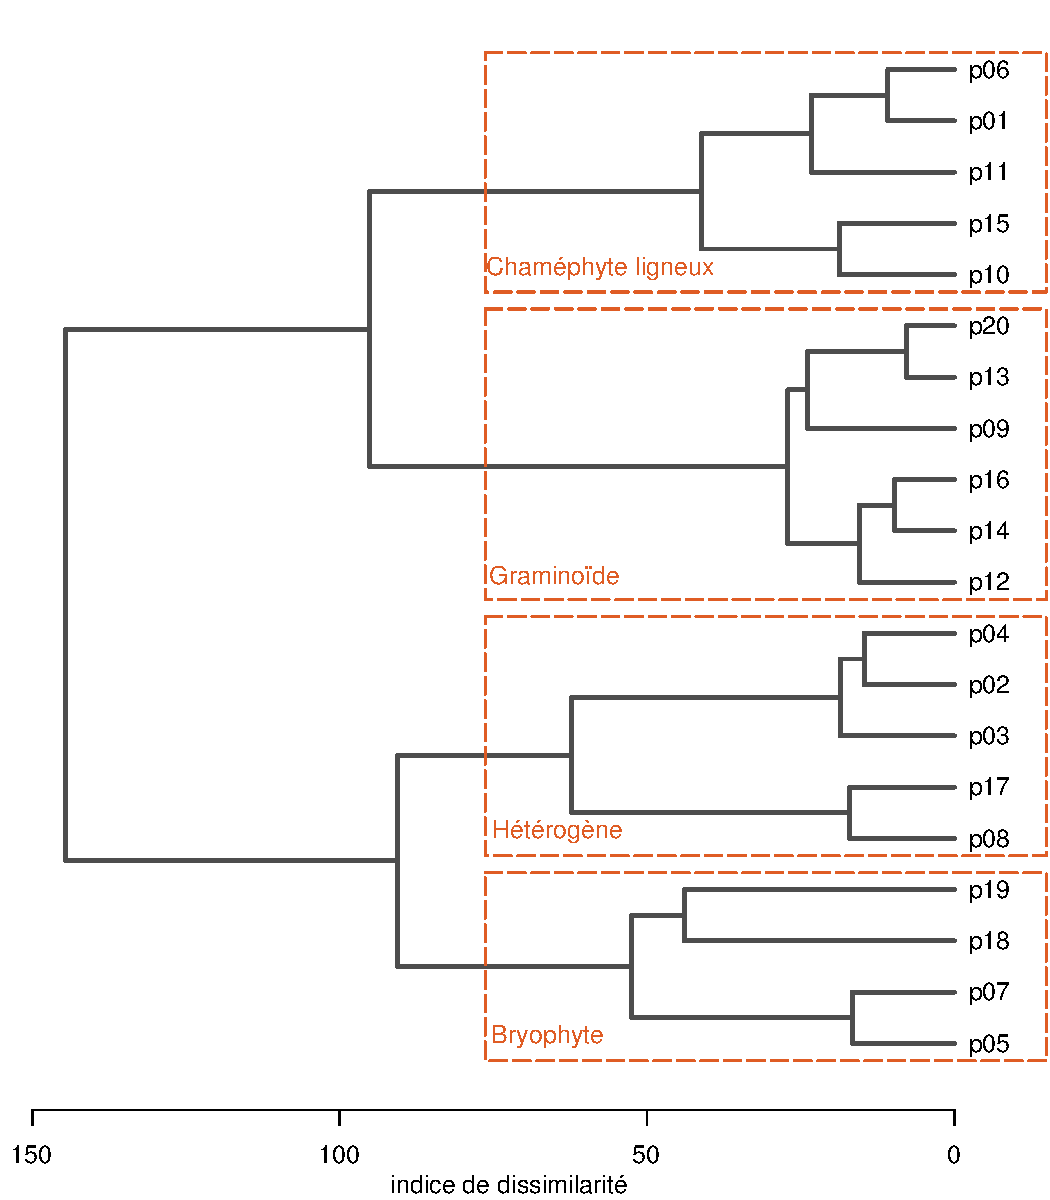
\includegraphics[width=.8\textwidth]{chap3/tree}
\caption{Partitionnement des placettes en fonction de leur similarité en termes de composition végétale (pourcentage des strates muscinales, herbacées et arbustives)}
\label{fig:tree}
\end{figure}


\subsection{Estimation de l'erreur associée aux flux et aux bilans}

Pour chaque flux, l'erreur sur le bilan annuel est calculé en multipliant ce flux par l'erreur quadratique normalisée, calculée lors de la calibration.
Pour les bilans, l'erreur associée est calculée comme la somme des erreurs associées aux flux composant le bilan.
Chacune de ces erreurs est pondérée en fonction de leur importance relative par rapport à la somme, en valeur absolue, des flux \citep{waddington2000}.

\begin{equation}
E_{(bilan)} = (\chi_{PPB} \times NRMSE_{PPB}) + (\chi_{RE} \times NRMSE_{RE}) + (\chi_{\fchh} \times NRMSE_{\fchh})
\end{equation}

Avec : 
\begin{itemize}
\item $E_{(bilan)}$ l'erreur associée au bilan
\item $\chi_{flux}$ la fraction du flux par rapport à la somme en valeurs absolue de tous les flux compris dans le bilan
\item $NRMSE_{flux}$ la racine carré de l'erreur quadratique normalisée à la moyenne associée au flux
\end{itemize}

Ces erreurs ne sont qu'une part de l'erreur totale qui devrait être associée à ces flux. Elle ne considère pas les erreurs aléatoires et systématiques liées aux mesures, qui sont supposées négligeable par rapport à l'erreur provenant de l'estimation des paramètres des équations et de la variablité spatiale des flux.


\section{Résultats}

\subsection{Cinétique des facteurs contrôlant et des flux de GES}

\subsubsection{Facteurs contrôlant}

\begin{figure}
\centering
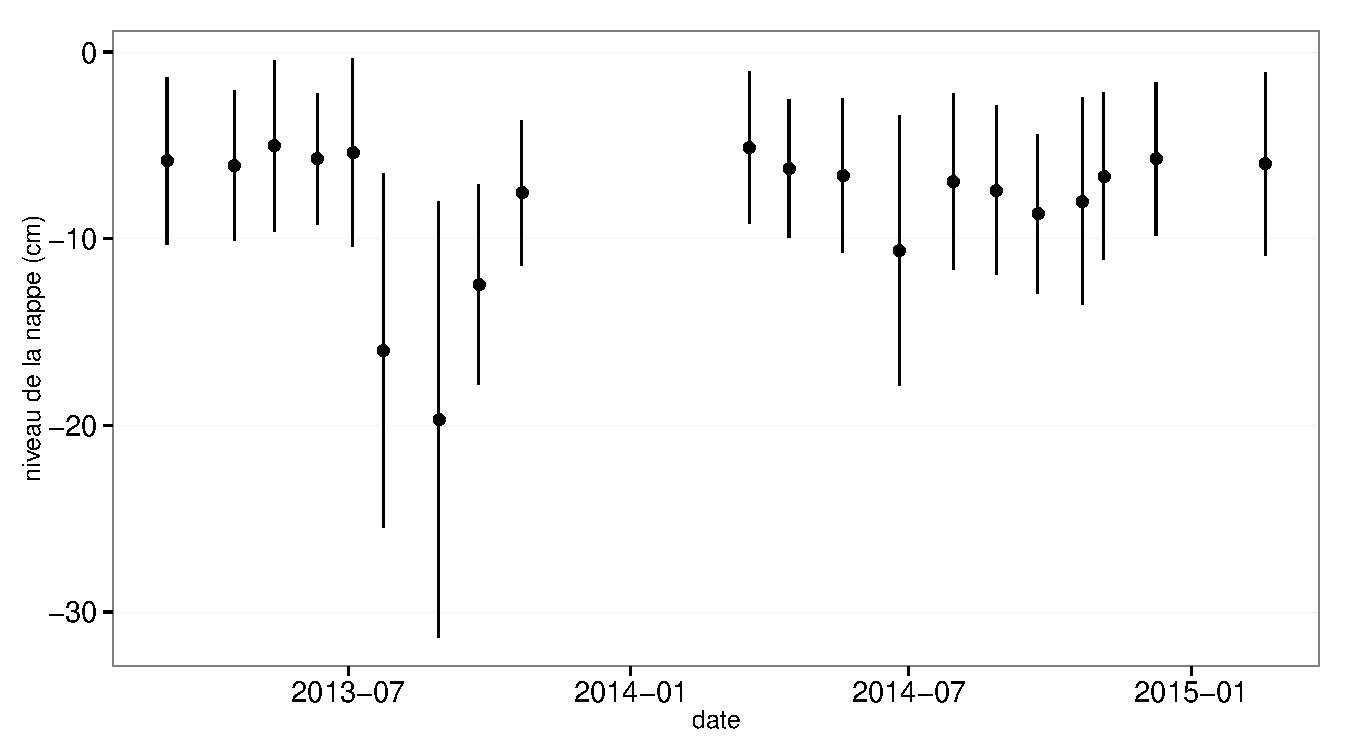
\includegraphics[width=1.15\textwidth, center]{chap3/WTL_mean_evolution}
\caption{Variabilité temporelle du niveau moyen de la nappe mesuré dans les 20 placettes entre mars 2013 et février 2015. Les valeurs correspondent à la distance entre le niveau de nappe et la surface du sol (en cm).}
\label{fig:WTL_mean_evolution}
\end{figure}

L'évolution du niveau de la nappe d'eau mesuré manuellement dans les 20 placettes est marquée par un étiage d'une vingtaine de centimètres en moyenne en 2013 et l'absence d'un étiage net en 2014 (Figure~\ref{fig:WTL_mean_evolution}).
Le niveau de la nappe moyen ne descend pas en dessous de \SI{-10}{\cm} avec \num{-9.2(76)} et \SI{-7.1(48)}{\centi\metre} respectivement pour 2013 et 2014.
% ne descendant que rarement sous la barre des \SI{-10}{\cm}.
Ces observations sont cohérentes avec les mesures acquises automatiquement et à plus haute fréquence (Figure~\ref{fig:WTL}), et confirment l'étiage particulièrement important de ces deux années par rapport aux précédentes.

\begin{figure}
\centering
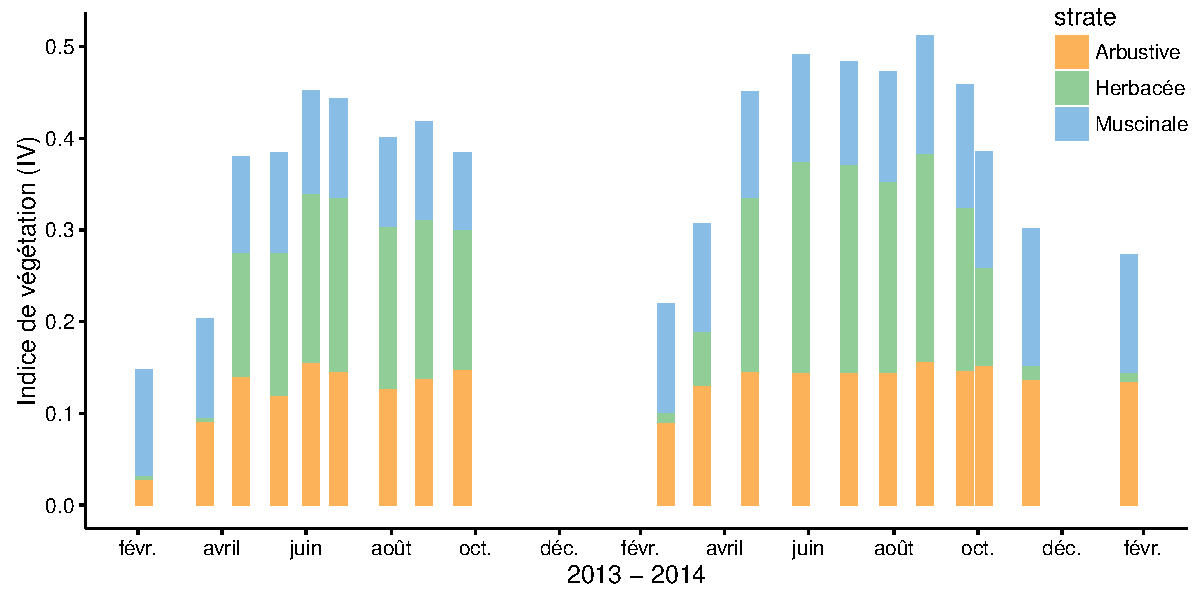
\includegraphics[width=1\textwidth, center]{chap3/veg_evol}
\caption{Variabilité de la valeur et de la composition (proportion des différentes strates végétales) de l'indice de végétation (IV) au cours du temps entre mars 2013 et février 2015, 
Évolution de la végétation à travers l'indice de végétation et des strates qui le compose}
\label{fig:veg_evol}
\end{figure}

L'évolution saisonnière de la végétation sur la tourbière de La Guette est visible (Figure~\ref{fig:veg_evol}).
Cette variabilité est majoritairement contrôlée par la strate herbacée qui meurt à la fin de la saison de végétation tandis que les arbustes et les mousses sont pérennes.
La saison de végétation, pour les herbacées, a commencé un peu plus tôt en 2014 (Figure~\ref{fig:veg_evol}) avec une végétation qui commence à croître en avril tandis qu'il faut attendre la campagne de mai en 2013.
L'indice de végétation est également légèrement plus important en 2014.

\begin{figure}
\centering
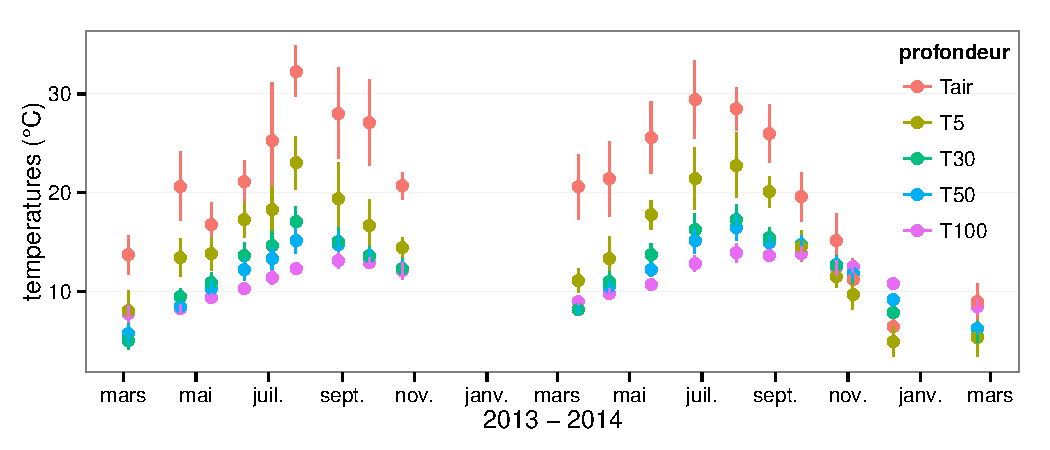
\includegraphics[width=1\textwidth, center]{chap3/T_mean_evolution}
\caption{Variabilité temporelle des moyennes des températures de l'air (Tair) et du sol à \SIlist{-5;-30;-50;-100}{\centi\metre} (T5, T30, T50 et T100 respectivement) mesurée dans les 20 placettes entre mars 2013 et février 2015}
\label{fig:T_mean_evolution}
\end{figure}

La température de l'air mesurée manuellement dans les 20 placettes montre une variabilité saisonnière comprise entre 6 et \SI{32}{\degreeCelsius} cohérente avec celle mesurée par la station météorologique. 
%bien que les valeurs semblent systématiquement supérieures.
La variabilité saisonnière de la température est également visible quand elle est mesurée dans le sol avec un amortissement et une diminution de la variabilité spatiale avec la profondeur : les températures varient de 5 à \SI{17}{\degreeCelsius} et de 8 à \SI{14}{\degreeCelsius} à \num{-30} et \SI{-100}{\centi\metre} respectivement (Figure~\ref{fig:T_mean_evolution}).
%chiffres ?

\begin{figure}
\centering
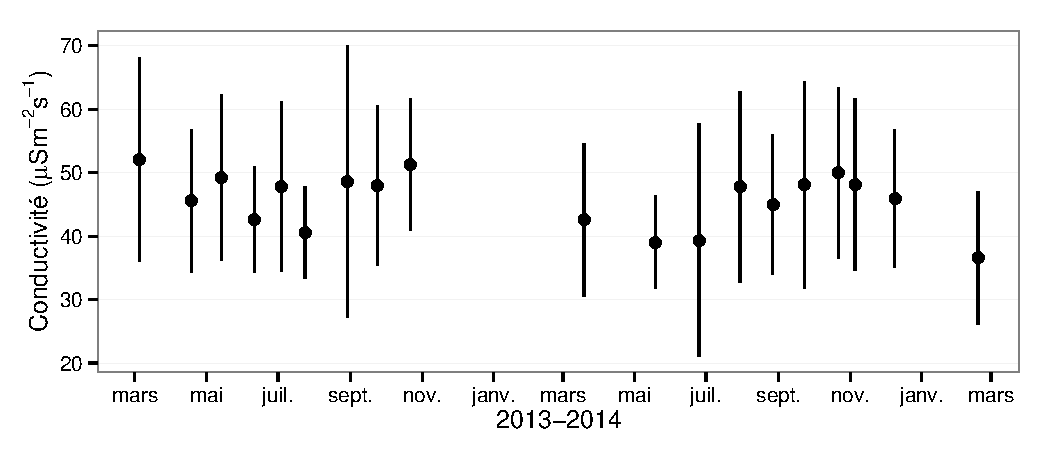
\includegraphics[width=1\textwidth, center]{chap3/cond_mean_evolution}
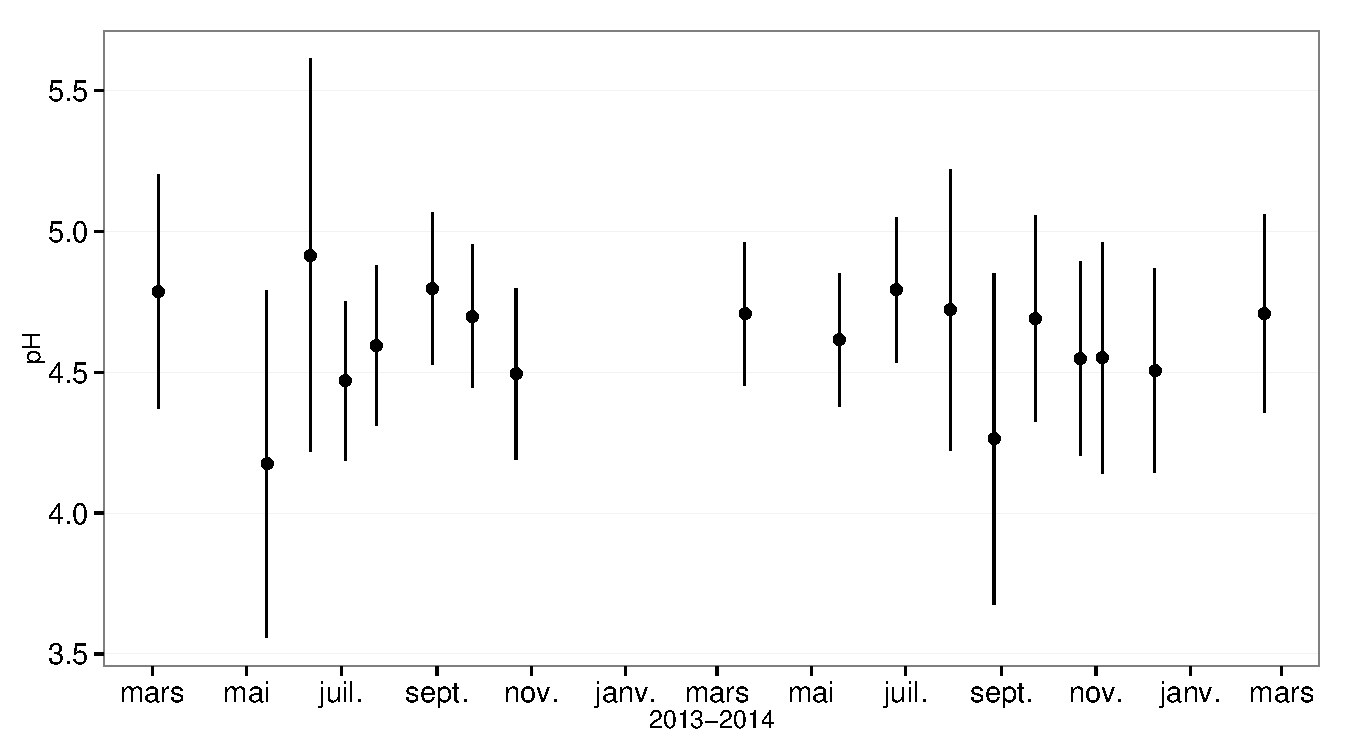
\includegraphics[width=1\textwidth, center]{chap3/pH_mean_evolution}
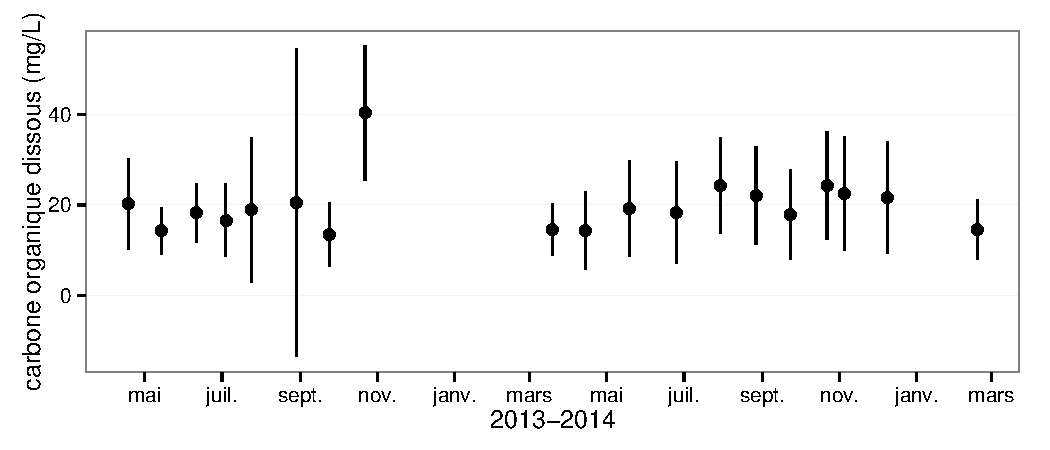
\includegraphics[width=1\textwidth, center]{chap3/NPOC_mean_evolution}
\caption{Variabilité temporelle des moyennes de la conductivité (A), du pH (B) et du carbone organique dissout (C) mesurés dans l'eau des piézomètres entre mars 2013 et février 2015.}
\label{fig:wtr_phychim}
\end{figure}



%
%\begin{figure}
%\centering
%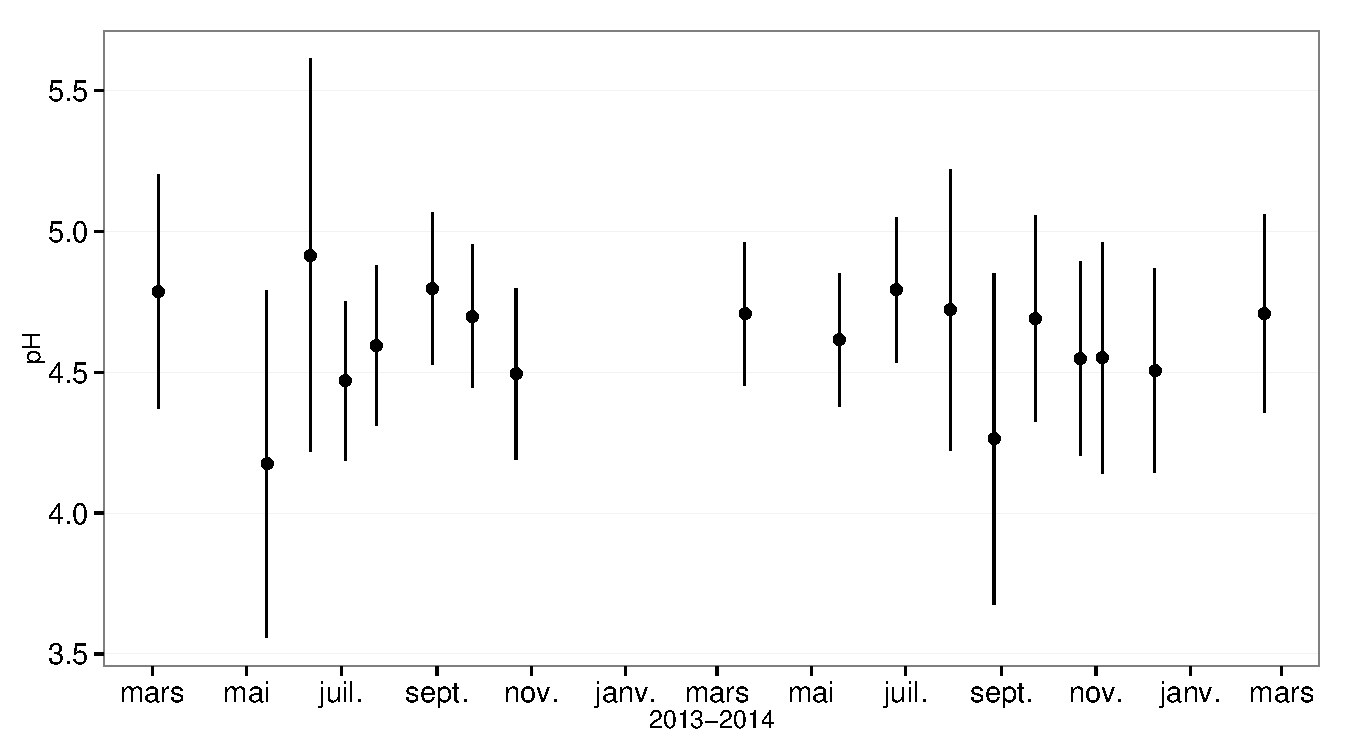
\includegraphics[width=\textwidth]{chap3/pH_mean_evolution}
%\caption{Évolution du pH pendant la période de mesure (mars 2013 -- février 2015)}
%\label{fig:pH_mean_evolution}
%\end{figure}

La conductivité moyenne mesurée dans l'eau des piézomètres des 20 placettes sur le site varie entre \num{35} et \SI{55}{\usml} (Figure~\ref{fig:wtr_phychim}--A).
En moyenne les valeurs de pH mesurées dans les placettes sont comprises entre 4 et 5 (Figure~\ref{fig:wtr_phychim}--B).
Ces valeurs sont cohérentes avec la classification en \textit{poor-fen} du site.
Les concentrations en carbone organique dissout des eaux prélevées dans les piézomètres sont comprises en moyenne entre \num{10} et \SI{30}{\milli\gram\per\liter} à l'exception d'un point en octobre 2013 (Figure~\ref{fig:wtr_phychim}--C).


%\begin{figure}
%\centering
%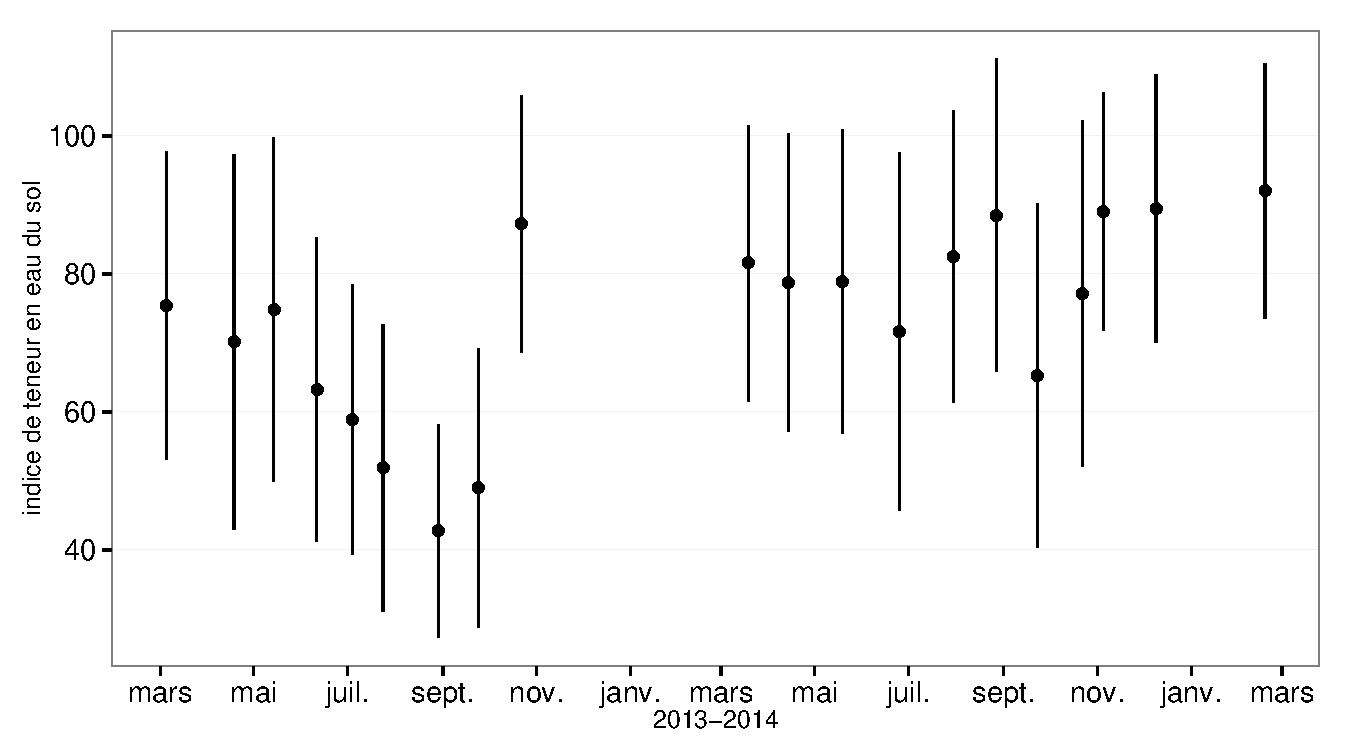
\includegraphics[width=\textwidth]{chap3/RH_mean_evolution}
%\caption{Évolution de la teneur en eau du sol pendant la période de mesure (mars 2013 -- février 2015)}
%\label{fig:RH_mean_evolution}
%\end{figure}

%\begin{figure}
%\centering
%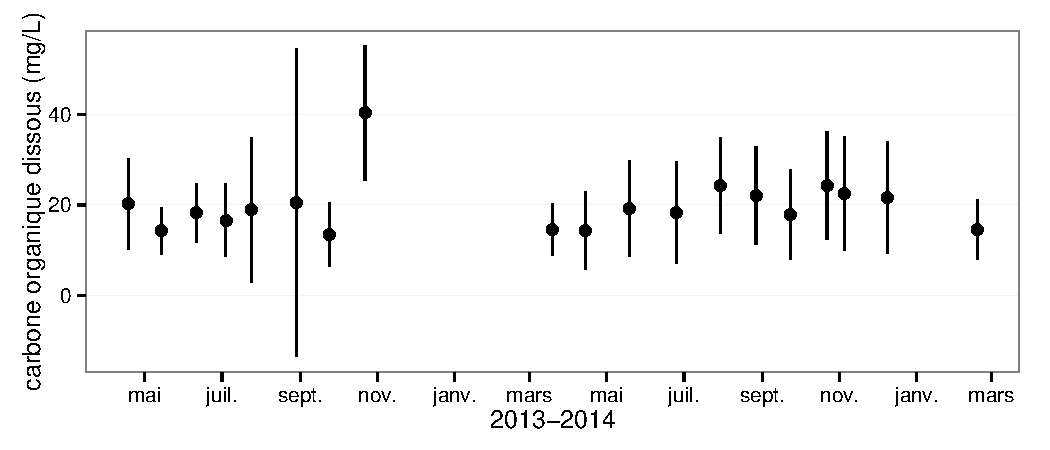
\includegraphics[width=\textwidth]{chap3/NPOC_mean_evolution}
%\caption{Évolution de la concentration en carbone organique dissous dans l'eau du sol pendant la période de mesure (mars 2013 -- février 2015)}
%\label{fig:NPOC_mean_evolution}
%\end{figure}


%\subsection{Évolution générale des flux de C sur la tourbière de La Guette}

\subsubsection{Flux de carbone}

\begin{figure}
	\centering
	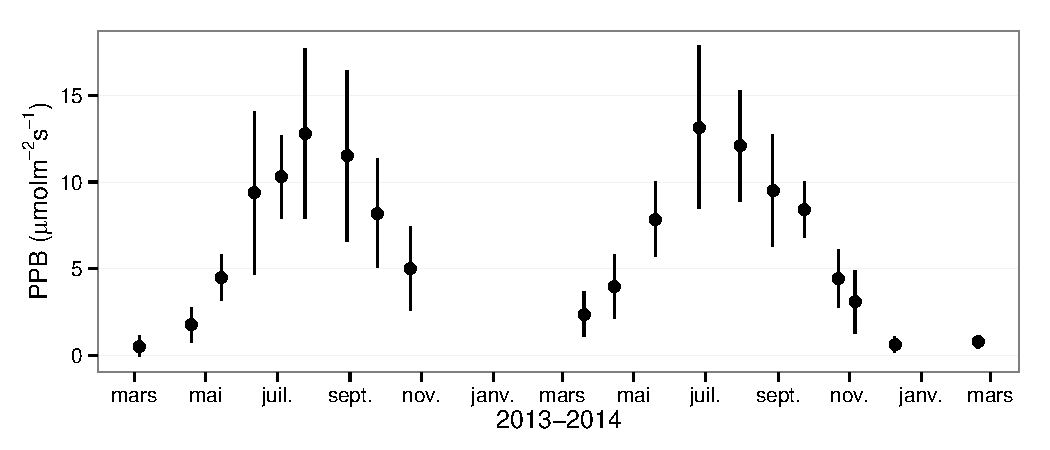
\includegraphics[width=1\textwidth, center]{chap3/GPP_evolution_avg}
	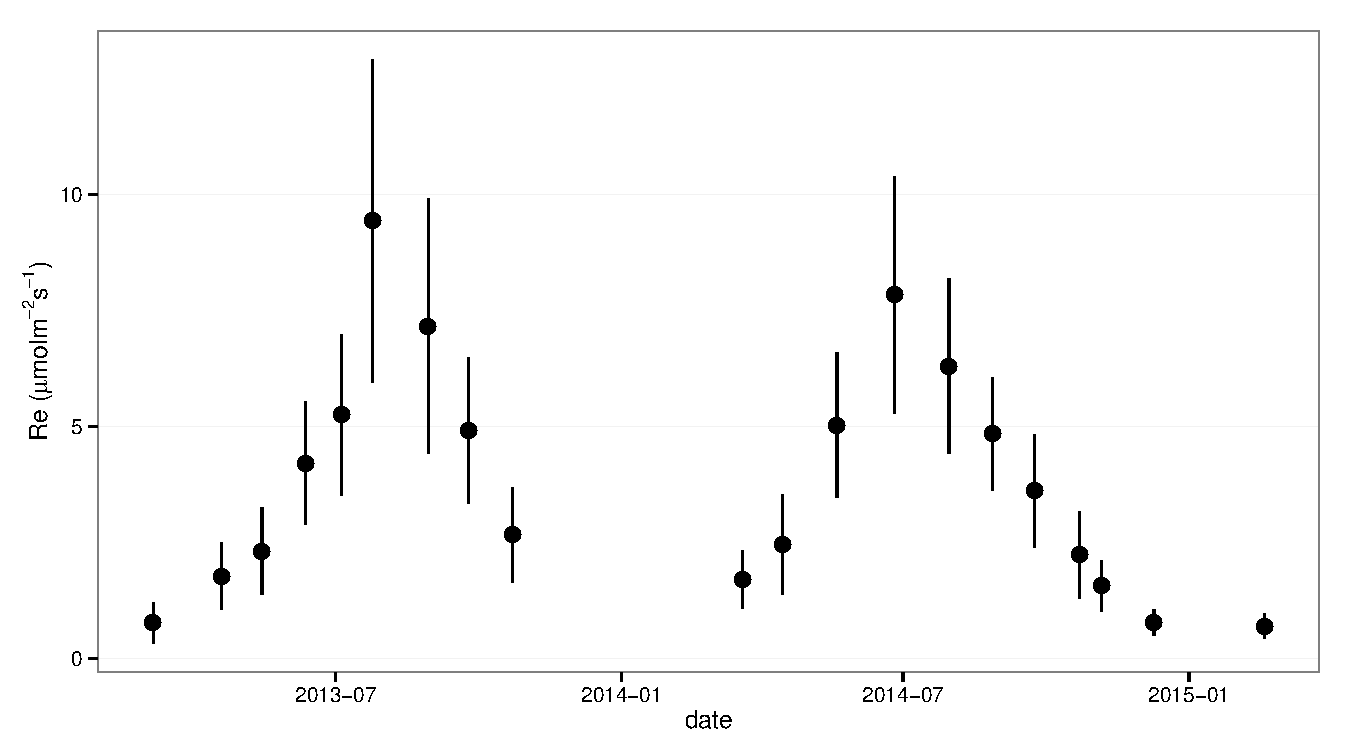
\includegraphics[width=1\textwidth, center]{chap3/ER_evolution_avg}
	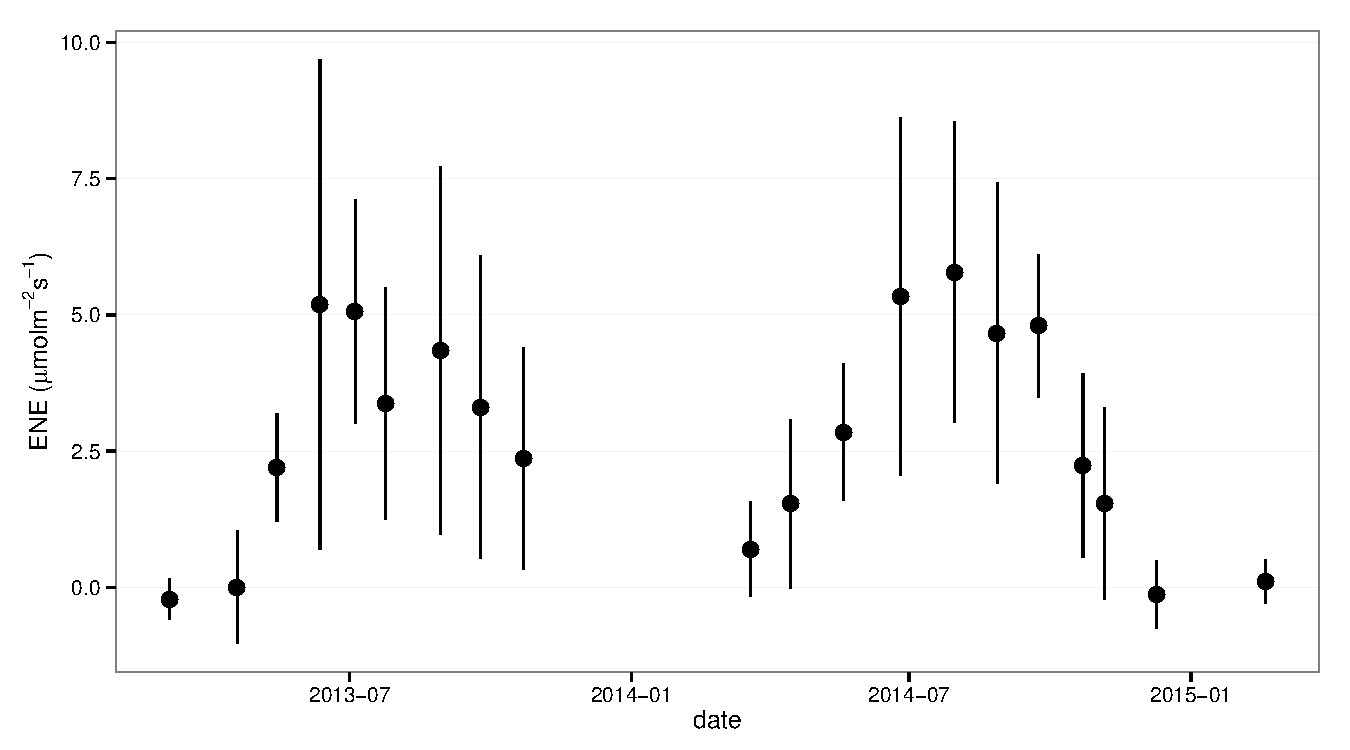
\includegraphics[width=1\textwidth, center]{chap3/NEE_evolution_avg}
\caption{Variabilité temporelle des flux de \coo moyen mesurés sur les 20 placettes entre mars 2013 et février 2015. Avec la PPB (A), la RE (B) et l'ENE (C) ; les barres d'erreur représentent la déviation standard.}
\label{fig:flux_evolution_avg}
\end{figure}

%\subsubsection{PBB}
Comme pour les facteurs contrôlant des mesures de \coo ont été effectuées de mars 2013 à février 2015.
De novembre 2013 à février 2014 les mesures ont été interrompue suite à des problèmes techniques.
Cependant les deux saisons de végétation, ont pu être mesurées dans leur ensemble, permettant d'avoir un jeu de données représentatif sur le fonctionnement de l'écosystème.

En 2013, les valeurs de la \textbf{PPB} (flux de \coo entrant dans l'écosystème) augmentent au printemps et une partie de l'été avec un maximum de \SI{12.80(491)}{\uml} atteint fin juillet, avant de diminuer à partir d'août (Figure~\ref{fig:flux_evolution_avg}--A).
En 2014 la PPB maximale est atteinte fin juin (\SI{13.16(470)}{\uml}), soit environ un mois plus tôt que l'année précédente.
Pendant la deuxième partie de l'été et l'automne les valeurs décroissent jusqu'à être proches de 0.
En moyenne les valeurs de la PPB sont de \SI{7.12(519)}{\uml} en 2013 et de \SI{6.56(472)}{\uml} en 2014.

La \textbf{RE} (flux de \coo sortant de l'écosystème) en 2013 augmente pendant le printemps et une partie de l'été (Figure~\ref{fig:flux_evolution_avg}--B).
Elle atteint \SI{9.43(348)}{\uml}, son maximum, en juillet avant de diminuer.
En 2014 la RE atteint, comme la PPB, son maximum plus tôt, en juin avec une valeur moyenne de \SI{7.83(255)}{\uml} avant de décroître en automne et en hiver ou elle approche de valeurs nulles.
Les valeurs moyennes de RE sont de \SI{4.27(316)}{\uml} en 2013, ce qui est légèrement supérieure à celle de 2014 : \SI{3.63(256)}{\uml}.

En 2013 les valeurs de l'\textbf{ENE} (bilan des flux de \coo entrant et sortant, les valeurs négative correspondent à une source de carbone et les valeurs positives à un puits) montrent un maximum en juin, atteignant \SI{5.19(451)}{\uml} puis elles diminuent jusqu'à la fin de l'année.
%Elles augmentent jusqu'à atteindre \SI{5.19(451)}{\uml}
%Concernant l'ENE (bilan des flux de \coo entrant et sortant), elle augmente en 2013 jusque \SI{5.19(451)}{\uml}, avec un maximum en juin, avant de diminuer jusqu'à la fin de l'année.
Cependant, cette baisse est moins uniforme que celle des deux flux précédents, avec notamment une augmentation de l'ENE entre juillet et août 2013.
%Ceci étant, il faut également noter les valeurs importantes de la déviation standard particulièrement en juin et en août.
En 2014, l'ENE maximum est atteinte en juillet avec \SI{5.79(277)}{\uml} (Figure~\ref{fig:flux_evolution_avg}--C).
%Cette baisse est cependant plus homogène qu'en 2013.
les valeurs moyennes annuelles de l'ENE sont très proches et sont de \SI{2.85(305)}{\uml} pour 2013 et \SI{2.93(277)}{\uml} pour 2014.
À noter également que pour l'ensemble des flux, la déviation standard augmente avec les valeurs mesurées.

%\subsubsection{Le \chh}

Les flux de \textbf{\chh}, comme ceux du \coo, montrent une variabilité saisonnière importante, même si les flux de \chh mesurés sont un ordre de grandeur en dessous de ceux mesurés pour le \coo (Figure~\ref{fig:CH4_evolution_avg}).
À l'inverse de ce dernier, les flux de \chh mesurés en 2013 sont nettement inférieurs à ceux mesurés en 2014 avec une moyenne de \num{0.04(003)} et de \SI{0.10(008)}{\uml} respectivement.
Les valeurs moyennes maximales atteignent \num{0.078} en 2013 et \SI{0.196}{\uml} en 2014.

\begin{figure}
\centering
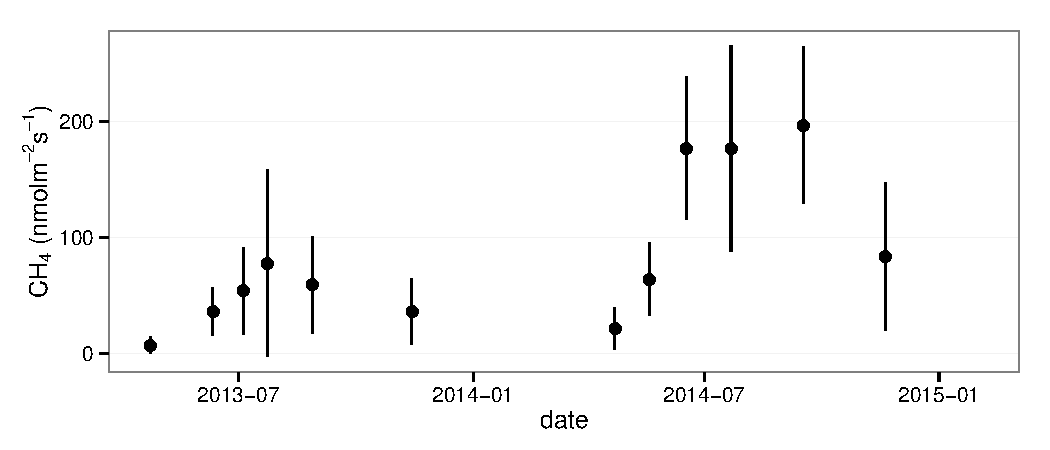
\includegraphics[width=1.15\textwidth, center]{chap3/CH4_evolution_avg}
\caption{Évolution des flux de méthane moyen sur cinq placettes entre mars 2013 et février 2015. les barres d'erreur représentent la déviation standard.}
\label{fig:CH4_evolution_avg}
\end{figure}

%\subsubsection{Le Carbone Organique Dissous (COD)}


\subsubsection{Relations entre flux gazeux et facteurs contrôlant}

\begin{figure}[!htb]
\centering
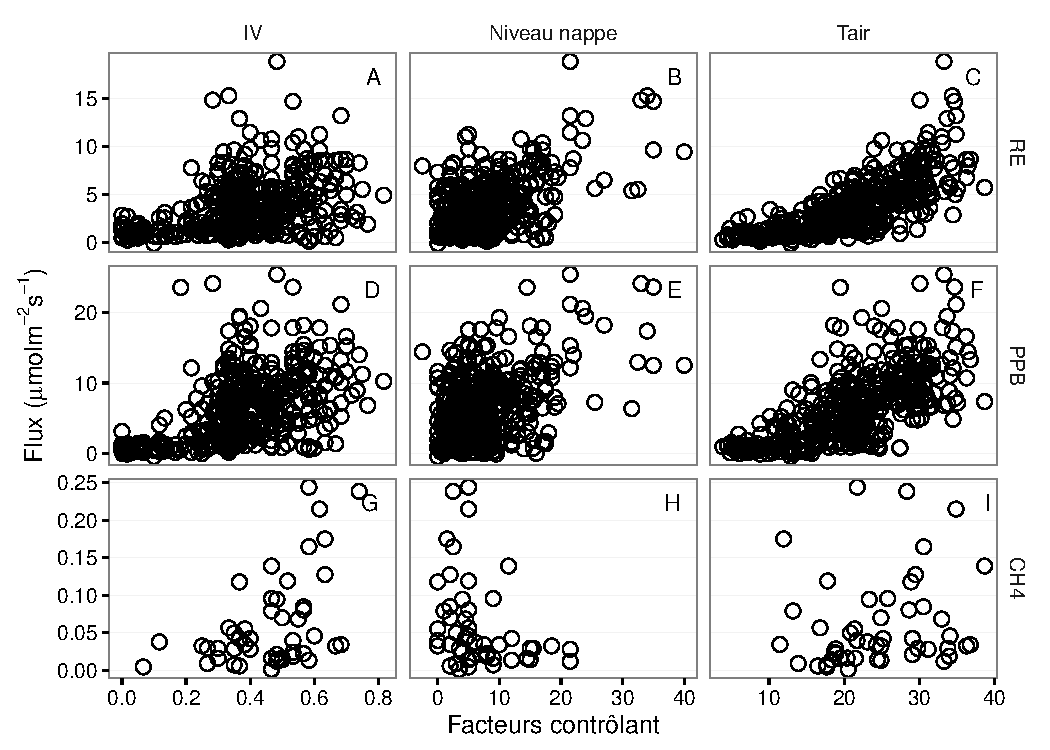
\includegraphics[width=\textwidth]{chap3/Fl_FC}
\caption{Relations entre les flux de gaz (exprimés en \si{\uml}) et une sélection de facteurs contrôlant : l'indice de végétation à droite (IV, sans unité), le niveau de la nappe d'eau au milieu (cm) et la température de l'air (Tair en \si{\degreeCelsius})}
\label{fig:Fl_FC}
\end{figure}

Comme précisé précédemment, le niveau de la nappe d'eau à très peu varié pendant les deux années de mesures, hormis un faible étiage d'août à octobre 2013.
De ce fait aucune relation claire n'est identifiable entre les flux et le niveau de la nappe que ce soit pour le \coo (PPB et RE) ou le \chh (Figure~\ref{fig:Fl_FC}--B,E et H).
La relation entre les flux de carbone (PPB et Re) et la température de l'air est de type exponentielle (Figure~\ref{fig:Fl_FC}--C et F).
%Le décrivent une tendance exponentielle.
Une tendance similaire est visible entre les flux de PPB et l'indice de végétation (IV), et dans une moindre mesure pour RE et \chh (Figure~\ref{fig:Fl_FC}--A,D et G).
Pour le \chh, aucune tendance n'est visible avec la température ou le niveau de la nappe, même si pour ce dernier il semble y avoir un maximum d'émission entre 0 et \SI{-10}{\centi\metre}.
Les flux de \chh montrent une tendance exponentielle avec l'indice de végétation.

L'ensemble de ces observations sont cohérentes avec les résultats des ACP (Annexe~\ref{sec:carbiodiv})
%La PPB et la RE présentent cependant des relations avec la température de l'air, et l'indice de végétation, même si pour ce dernier les tendances sont moins claires, particulièrement pour la RE (Figure~\ref{fig:Fl_FC}).
%Le \chh ne montre pas de relation avec la température de l'air, mais une tendance exponentielle est visible vis-à-vis de l'indice de végétation (Figure~\ref{fig:Fl_FC}).
%\textbf{(\chh et Température dans la tourbe ?)}

\subsection{Estimation des flux de GES}

\subsubsection{Production primaire brute}


L'estimation de la PPB se fait en deux étapes.
Dans un premier temps on estime le potentiel maximum de photosynthèse à un instant donné dans des conditions de lumière saturante (PPBsat).
Ce potentiel peut varier avec les conditions environnementales et a été déterminé en utilisant une équation qui relie la vitesse de transport des électrons photosynthétiques à lumière saturante à la température \citep{june2004} :

\begin{equation}\label{eq:juneTair}
PPBsat = a * exp\left(\frac{Tair - b}{c}\right)^2
\end{equation}

Avec :
\begin{itemize}
\item $a$ : vitesse de transport des électrons photosynthétique à lumière saturante (\si{\uml})
\item $b$ : température optimale pour ce transport (\si{\degreeCelsius})
\item $c$ : différence de température à laquelle à laquelle PBBsat vaut e$^{-1}$ de sa valeur à la température optimale (\si{\degreeCelsius})
\end{itemize}

À partir de ce potentiel à lumière saturante, la PPB est estimée en prenant en compte la luminosité.
On a utilisé l'équation~\ref{eq:PPB_bubier} proposée par \citep{bubier1998} et utilisée par de nombreux auteurs \citep{bortoluzzi2006a,worrall2009}:

\begin{equation} \label{eq:PPB_bubier}
PPB = \frac{PPBsat * i * PAR}{PPBsat + i * PAR}
\end{equation}

\begin{figure} %[!htb]
\centering
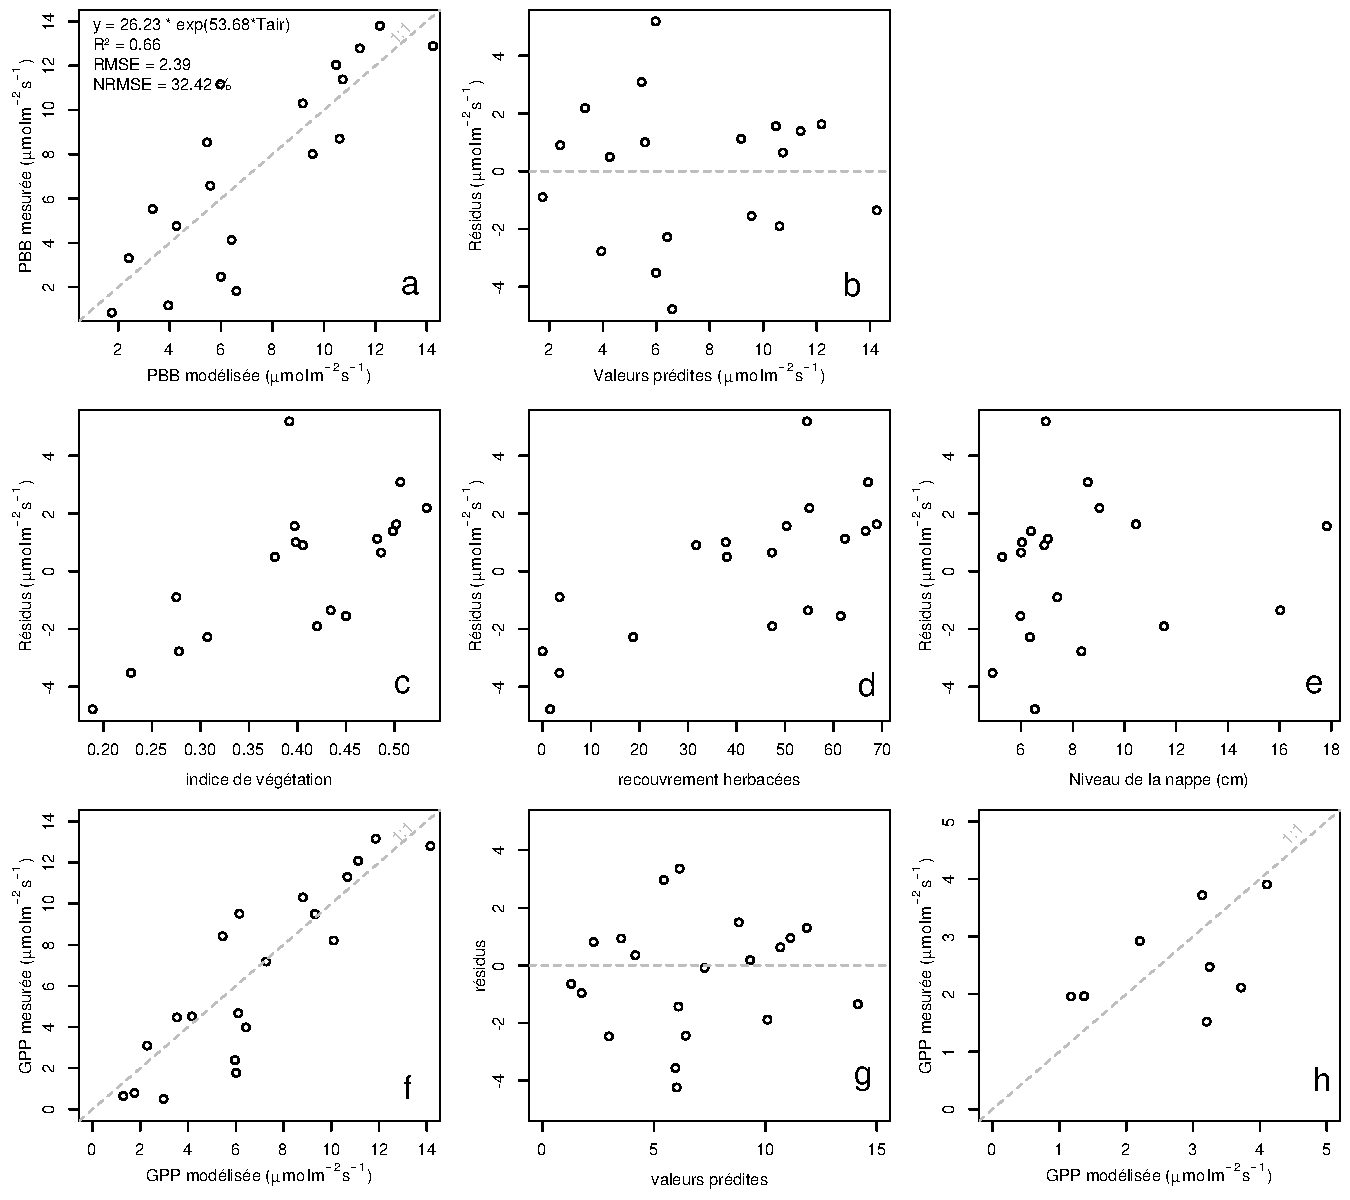
\includegraphics[width=1.15\textwidth, center]{chap3/mdl_GPP_Tair}
\caption{Résultats de la calibration de la PPB. En haut la PPBsat (équation~\ref{eq:juneTair} avec la représentativité du modèle et la distribution des résidus (graphes a et b). Au milieu les tendances entre les résidus de cette équation et l'indice de végétation, le pourcentage de recouvrement de la strate herbacée et le niveau de la nappe (graphes c, d et e). Et en bas la PPB (équation~\ref{eq:PPB_bubier}), sa représentativité et la distribution des résidus de l'équation (graphes f et g) et l'évaluation sur un jeu de données indépendant (graphe h, annexe~\ref{sec:carbiodiv})).}
\label{fig:mdl_GPP_Tair}
\end{figure}

L'utilisation de l'équation de June seule, avec la température de l'air comme variable explicative de la PPBsat, permet d'expliquer 66 \% des variations observées avec une NRMSE de \SI{32}{\percent} (Figure~\ref{fig:mdl_GPP_Tair}-a).
Les résidus de ce modèle se répartissent de façon relativement homogène et non biaisée (Figure~\ref{fig:mdl_GPP_Tair}-b).
Corrélés avec l'indice de végétation IV, ils présentent une tendance linéaire croissante (Figure~\ref{fig:mdl_GPP_Tair}-c).
On observe la même tendance avec le recouvrement de la strate herbacée avec une dispersion des points plus importante (Figure~\ref{fig:mdl_GPP_Tair}-d).
Par contre aucune relation n'est visible avec le niveau de la nappe d'eau (Figure~\ref{fig:mdl_GPP_Tair}-e)
Le pourcentage de recouvrement des sphaignes (non présenté) ne montre également, aucune tendance avec les résidus de cette équation.
La PPB calculée à partir des équations~\ref{eq:juneTair} et \ref{eq:PPB_bubier} a une NRMSE de \SI{31}{\percent}, du même ordre de grandeur que celle de PPBsat (Figure~\ref{fig:mdl_GPP_Tair}-f) et les résidus se répartissent de façon relativement homogène et non biaisée (Figure~\ref{fig:mdl_GPP_Tair}-g).
Cependant l'évaluation du modèle sur les données de tests a une NRMSE plus forte qui atteint \SI{47}{\percent}(Figure~\ref{fig:mdl_GPP_Tair}-h).
Par ailleurs une forte incertitude est présente concernant l'estimation des paramètres qui ont tous une erreur standard importante, (parfois plus importante que la valeur du paramètre), et une faible significativité (Tableau~\ref{table:mdl_par}).
Afin de prendre en compte la tendance linéaire entre les résidus et l'indice de végétation (IV) nous avons adapté le modèle, à la manière de \citet{bortoluzzi2006a}, pour y intégré une fonction linéaire de la végétation :

\begin{equation}\label{eq:juneTairIV}
PPBsat = (a * IV + d) * exp\left(\frac{T - b}{c}\right)^2
\end{equation}

\begin{figure} %[!htb]
\centering
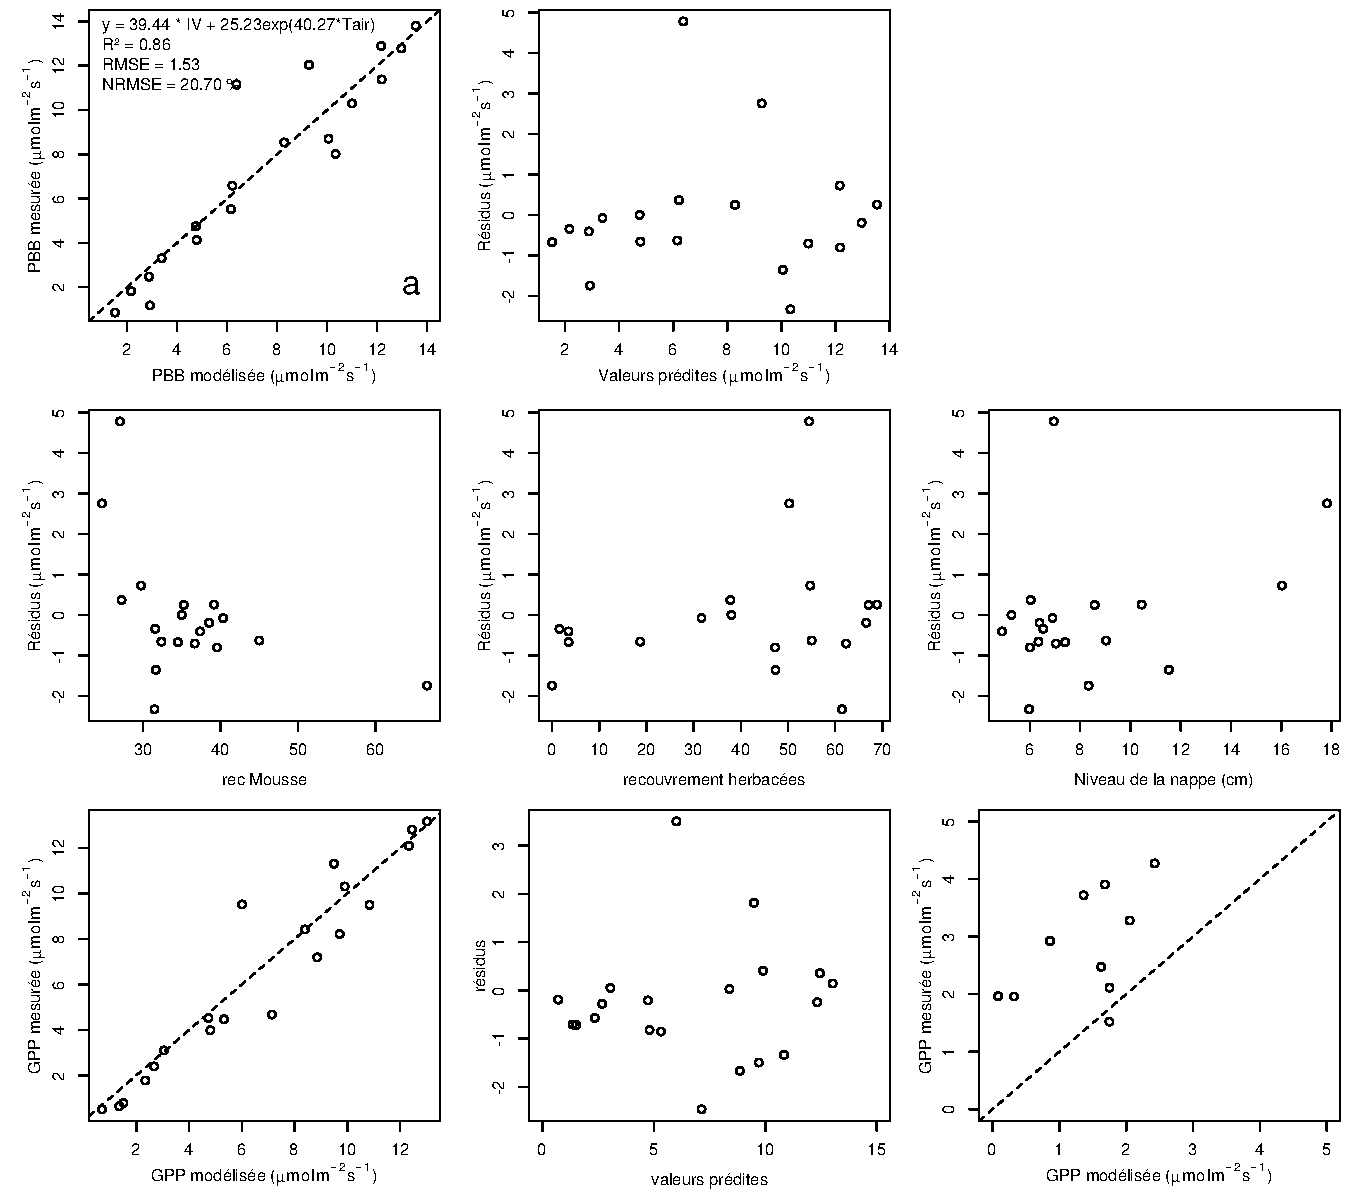
\includegraphics[width=1.15\textwidth, center]{chap3/mdl_GPP_TairIV}
\caption{Résultats de la calibration de la PPB en prenant en compte la végétation. En haut la PPBsat (équation~\ref{eq:juneTairIV} avec la représentativité du modèle et la distribution des résidus (graphes a et b). Au milieu les tendances entre les résidus de cette équation et l'indice de végétation, le pourcentage de recouvrement de la strate herbacée et le niveau de la nappe (graphes c, d et e). Et en bas la PPB (équation~\ref{eq:PPB_bubier}), sa représentativité et la distribution des résidus de l'équation (graphes f et g) et l'évaluation sur un jeu de données indépendant (graphe h, annexe~\ref{sec:carbiodiv}).}
\label{fig:mdl_GPP_TairIV}
\end{figure}

Cette nouvelle équation permet d'expliquer une part plus importante des variations de PPBsat (R$^{2}$ = 0,85) et augmente la proximité entre les données mesurées et les données modélisées : la NRMSE diminue à \SI{21}{\percent}. (Figure~\ref{fig:mdl_GPP_TairIV}-a).
Les résidus de cette équation semblent répartis de façon moins homogène que précédemment.
Avec notamment un resserrement des points autour de zéro à l'exception d'un point de valeur supérieur à \num{4} (Figure~\ref{fig:mdl_GPP_TairIV}-b).
Le biais reste malgré tout faible au regard de l'amélioration apportée.
Aucune tendance claire ne se dégage des résidus lorsqu'ils sont mis en relation avec des facteurs contrôlant tels que les recouvrements végétaux (que ce soit celui des sphaignes ou des herbacées), ou le niveau de la nappe d'eau (Figure~\ref{fig:mdl_GPP_TairIV}--c,d,e).
Comme précédemment, la NRMSE de la PPB, de \SI{19}{\percent}, est du même ordre de grandeur que celle de PPBsat (Figure~\ref{fig:mdl_GPP_TairIV}--f).
La NRMSE de PPBsat et PPB diminue avec la prise en compte de l'indice de végétation lors de la calibration.
En revanche, l'évaluation sur les données de test de ce dernier modèle montre une NRMSE importante (\SI{58}{\percent}), supérieure à celle du modèle ne prenant pas en compte la végétation (Figure~\ref{fig:mdl_GPP_TairIV}--h).
Cette évaluation montre également une tendance importante à sous-estimer les valeurs mesurées.
Néanmoins ce modèle intégrant la végétation permet de diminuer de façon importante l'erreur associée à l'estimation des paramètres de l'équation.

Dans la suite du texte le modèle permettant d'estimer la PPB à partir des équations~\ref{eq:juneTair} et \ref{eq:PPB_bubier} sera nommé \textbf{PPB-1} et celui utilisant les équations~\ref{eq:PPB_bubier} et \ref{eq:juneTairIV} sera nommée \textbf{PPB-2}.


\begin{table}
\centering
\caption{Valeur des paramètres des équations utilisées pour modéliser les flux et sensibilité relative (en \%) des flux en réponse à une variation de $\pm$\SI{10}{\percent} de chacun des paramètres des modèles.}
\label{table:mdl_par}
\begin{tabular}{llcccccc}\toprule

& par & valeur & se & pval & \SI{-10}{\percent} & +\SI{+10}{\percent} & AIC \\ \midrule
\multicolumn{7}{l}{PPB-1 -- équations~\ref{eq:juneTair} et \ref{eq:PPB_bubier}} & 95 \\ [+.5ex]
& a & 26.23 & 62.07 & 0.68 & -9.7 & +9.6 & \\
& b & 53.68 & 61.27 & 0.39 & +43.7 &-35.1 & \\
& c & 27.21 & 28.56 & 0.35 &-22.5 & +21.9 & \\
& i &  1.84 & 21.6  & 0.93 & -0.4 &  +0.4 & \\[+1ex]
\multicolumn{7}{l}{PPB-2 -- équations~\ref{eq:juneTairIV} et \ref{eq:PPB_bubier}} & 80 \\ [+.5ex]
& a & 39.44 & 18.89 & 0.05 & -11.8 & +11.5 &\\
& b & 40.27 & 19.11 & 0.05 & +15.8 & -17.2 &\\
& c & 25.23 & 14.35 & 0.1 & -8.1 & +6.7 &\\
& d & -3.73 & 3.49 & 0.3 & +2.8 & -2.8 &\\
& i &  0.26 & 0.25 & 0.31 & -1.3 & +1.1 &\\[+1ex]
\multicolumn{7}{l}{RE-1 -- équation~\ref{eq:RE_T}} & 47 \\ [+.5ex]
& a & 0.34 & 0.08 & 0 & -10 & +10 &\\
& b & 0.10 & 0.01 & 0 & -22.6 & +29.9 &\\[+1ex]
\multicolumn{7}{l}{RE-2 -- équation~\ref{eq:RE_TIV}} & 37 \\ [+.5ex]
& a & 0.92 & 0.34 & 0.02 & -7.3 & +7.3 &\\
& b & 0.09 & 0.01 & 0.00 & -19.5 & 24.7 &\\
& c & 0.14 & 0.09 & 0.14 & +2.7 & -2.7  &\\[+1ex]
\multicolumn{7}{l}{RE-3 -- équation~\ref{eq:RE_TH}} & 35  \\ [+.5ex]
& a & 0 & 0 & 0.01 & -3.9 & +3.9 &\\
& b & 0.08 & 0.01 & 0 & -18.8 & +23.6 &\\
& c & 0.33 & 0.06 & 0 & -6.1 & +6.1 &\\[+1ex]
\multicolumn{7}{l}{FCH4 -- équation~\ref{eq:CH4_H}}  &\\ [+.5ex]
& a & 0 & 0 & 0.48 & -10 & +10 &\\
& b & 13.01 & 2.82 & 0 & -43.9 & +79.2 & \\[+1ex]
\bottomrule
\end{tabular}
\end{table}

\subsubsection{Respiration de l'écosystème}

\begin{figure} %[!htb]
\centering
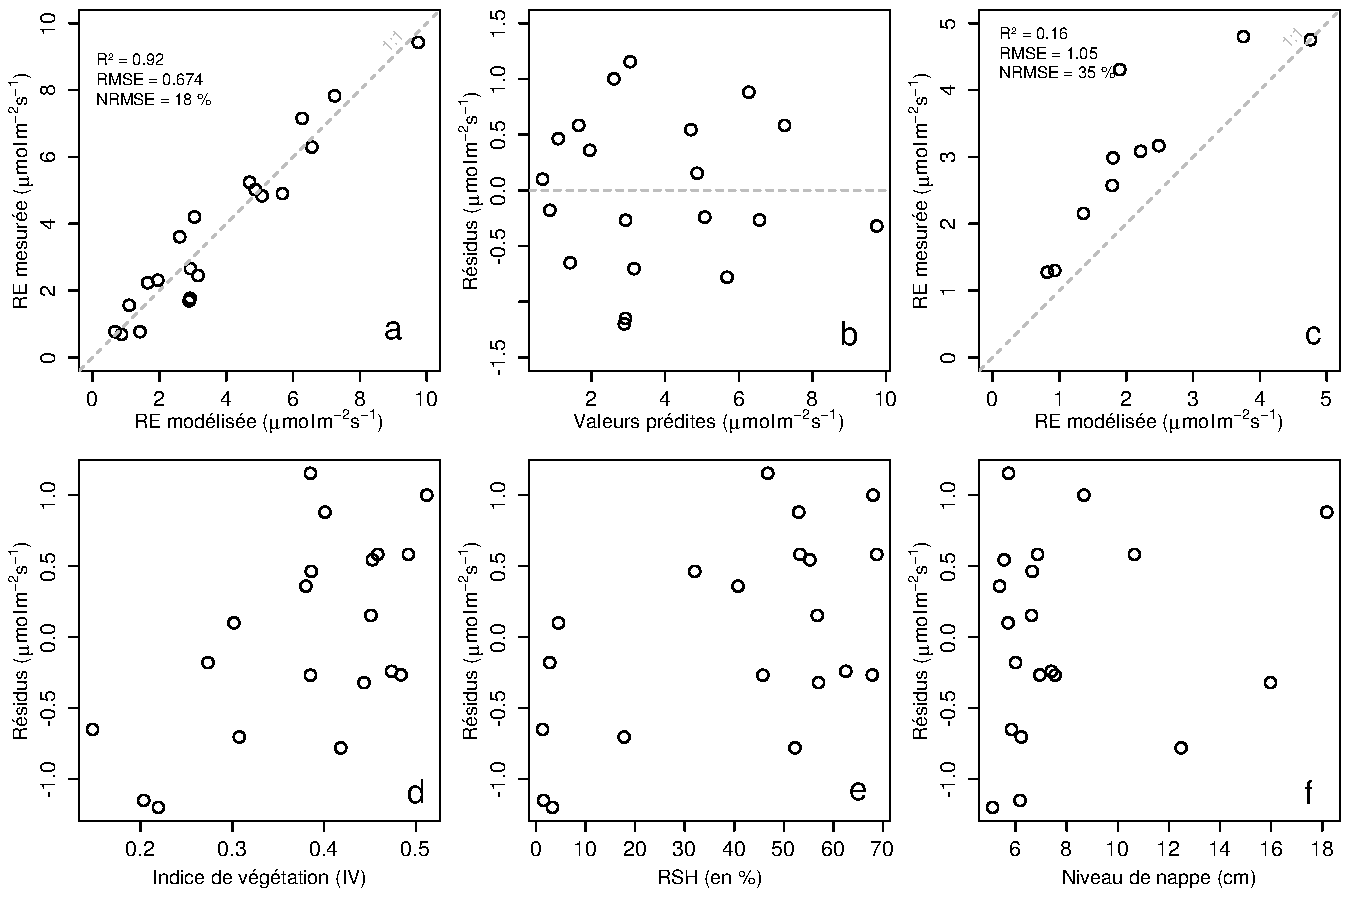
\includegraphics[width=1.05\textwidth, center]{chap3/mdl_ER_Tair}
\caption{\label{fig:mdl_ER_Tair}
Calibration de la RE utilisant l'équation~\ref{eq:RE_T}. En haut la représentativité du modèle et la distribution des résidus (graphes a et b), ainsi que son évaluation sur un jeu de données indépendant (graphe c, annexe~\ref{sec:carbiodiv})). En bas les tendances entre les résidus de cette équation et l'indice de végétation, le pourcentage de recouvrement de la strate herbacée et le niveau de la nappe (graphes c, d et e).}
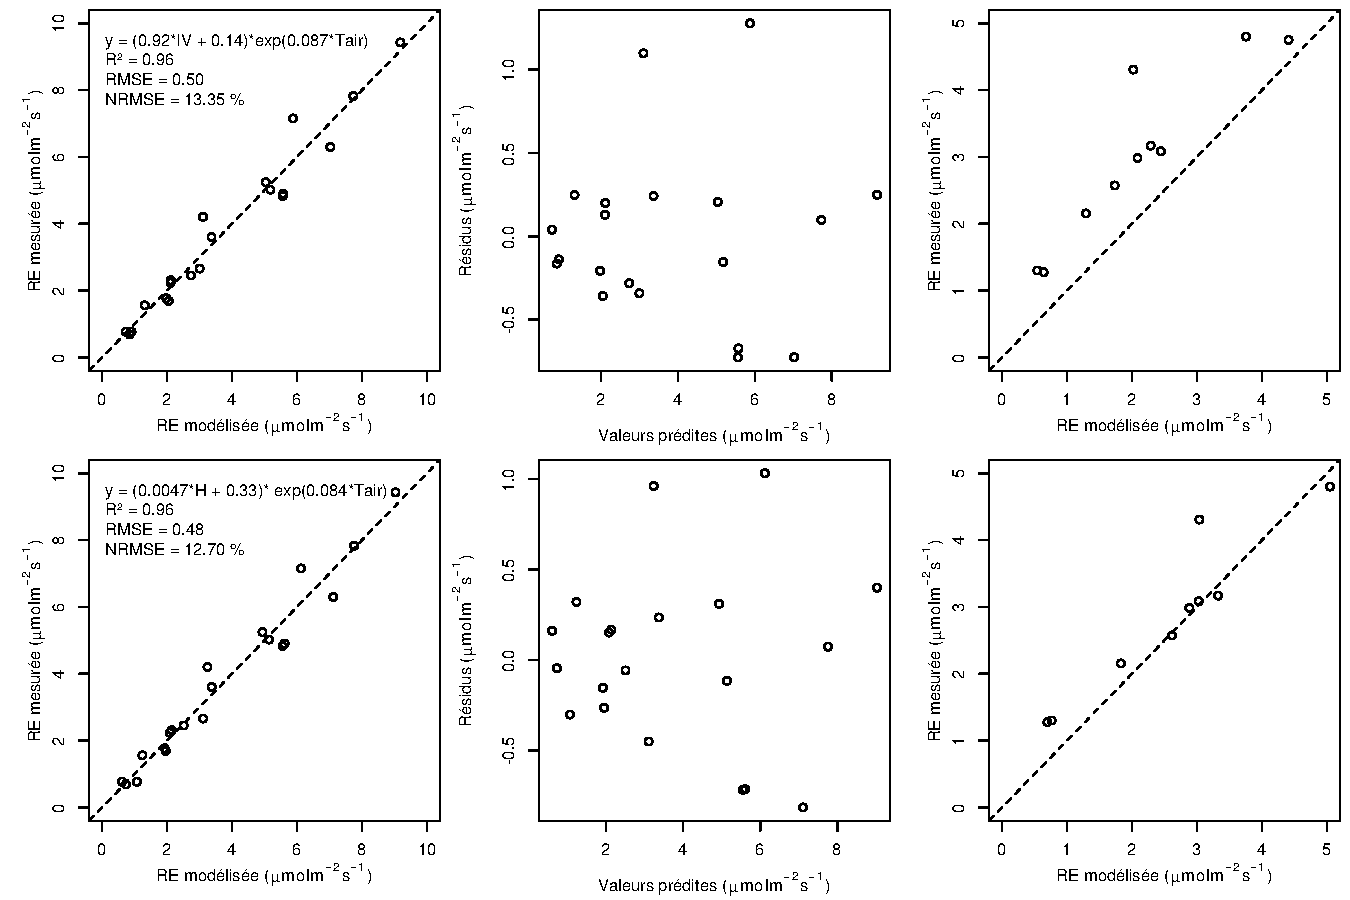
\includegraphics[width=1.05\textwidth, center]{chap3/mdl_ER_Tair_IVH}
\caption{\label{fig:ER_mdl_TairIVH}Calibration de la RE prenant en compte la végétation en utilisant l'équation~\ref{eq:RE_TIV}, en haut, et l'équation~\ref{eq:RE_TH} en bas. Avec la représentativité des modèles et la distribution de leurs résidus (graphes a et b pour le premier et d et e pour le second), ainsi que leur évaluation sur un jeu de données indépendant (graphe c et f, annexe~\ref{sec:carbiodiv})).}
\end{figure}

La relation exponentielle entre la RE et la température est reconnue \citep{luo2006}, et la RE est estimée avec l'équation :
%L'estimation de la RE s'effectue avec l'équation :

\begin{equation} \label{eq:RE_T}
RE = a*exp(b*T)
\end{equation}

La température de l'air utilisée dans un modèle exponentiel permet d'expliquer \SI{90}{\percent} des variations de la respiration de l'écosystème avec une NRMSE de \SI{18}{\percent} (Figure~\ref{fig:mdl_ER_Tair}--a).
Les résidus de cette équation sont répartis de façon non-biaisée (Figure~\ref{fig:mdl_ER_Tair}--b).
L'évaluation de ce modèle montre une NRMSE de \SI{35}{\percent} avec une tendance à sous-estimer les valeurs mesurées (Figure~\ref{fig:mdl_ER_Tair}--c).
Une légère tendance, est visible entre les résidus et l'indice de végétation ainsi qu'avec le recouvrement de la strate herbacée (Figure~\ref{fig:mdl_ER_Tair}--d,e) mais pas avec le niveau de la nappe (Figure~\ref{fig:mdl_ER_Tair}--f).
Très souvent utilisée, la température à \SI{-5}{\centi\metre} donne des résultats proches mais moins bons notamment avec une hétéroscédasticité des résidus (Annexe~\ref{sec:calib_flux}, figure~\ref{fig:RE_T5}).
%Dans les deux cas, le gain possible en ajoutant un paramètre semble limité.
On adapte l'équation~\ref{eq:RE_T} pour intégrer le signal de végétation de deux façon, avec l'IV :

\begin{equation} \label{eq:RE_TIV}
RE = (a*IV + c)*exp(b*T)
\end{equation}

Et avec le seul pourcentage de recouvrement des herbacées (RSH) qui contrôle en grande partie l'IV (Figure~\ref{fig:veg_evol})

\begin{equation} \label{eq:RE_TH}
RE = (a*RSH + c)*exp(b*T)
\end{equation}

Les calibrations de ces nouvelles équations sont présentées dans la figure~\ref{fig:ER_mdl_TairIVH}-a,b et \ref{fig:ER_mdl_TairIVH}-d,e respectivement.
Dans les deux cas, la NRMSE diminue pour avoisiner \SI{13}{\percent}, avec des résidus qui se répartissent de façon non-biaisée.
L'évaluation de ces deux équations montre cependant des différences :
D'une part l'équation~\ref{eq:RE_TIV} ne permet pas de diminuer la NRMSE (\SI{34}{\percent}) et est très proche des \SI{35}{\percent} calculé pour l'évaluation du modèle n'intégrant pas la végétation (Figure~\ref{fig:ER_mdl_TairIVH}--c).
D'autre part l'évaluation de l'équation~\ref{eq:RE_TH} montre une NRMSE plus faible de \SI{23}{\percent} (Figure~\ref{fig:ER_mdl_TairIVH}--f).
Les paramètres des différentes équations sont présentés dans le tableau~\ref{table:mdl_par} ; les modèles \textbf{RE-1}, \textbf{RE-2}, et \textbf{RE-3} correspondent respectivement aux équations~\ref{eq:RE_T}, \ref{eq:RE_TIV} et \ref{eq:RE_TH}.
À l'inverse de la PPB les paramètres des modèles de la RE ont, à l'exception du paramètre c du modèle RE-2, une significativité importante (p-value < 0,05) et une NRMSE faible (Tableau~\ref{table:mdl_par}).



%\begin{figure}
%\centering
%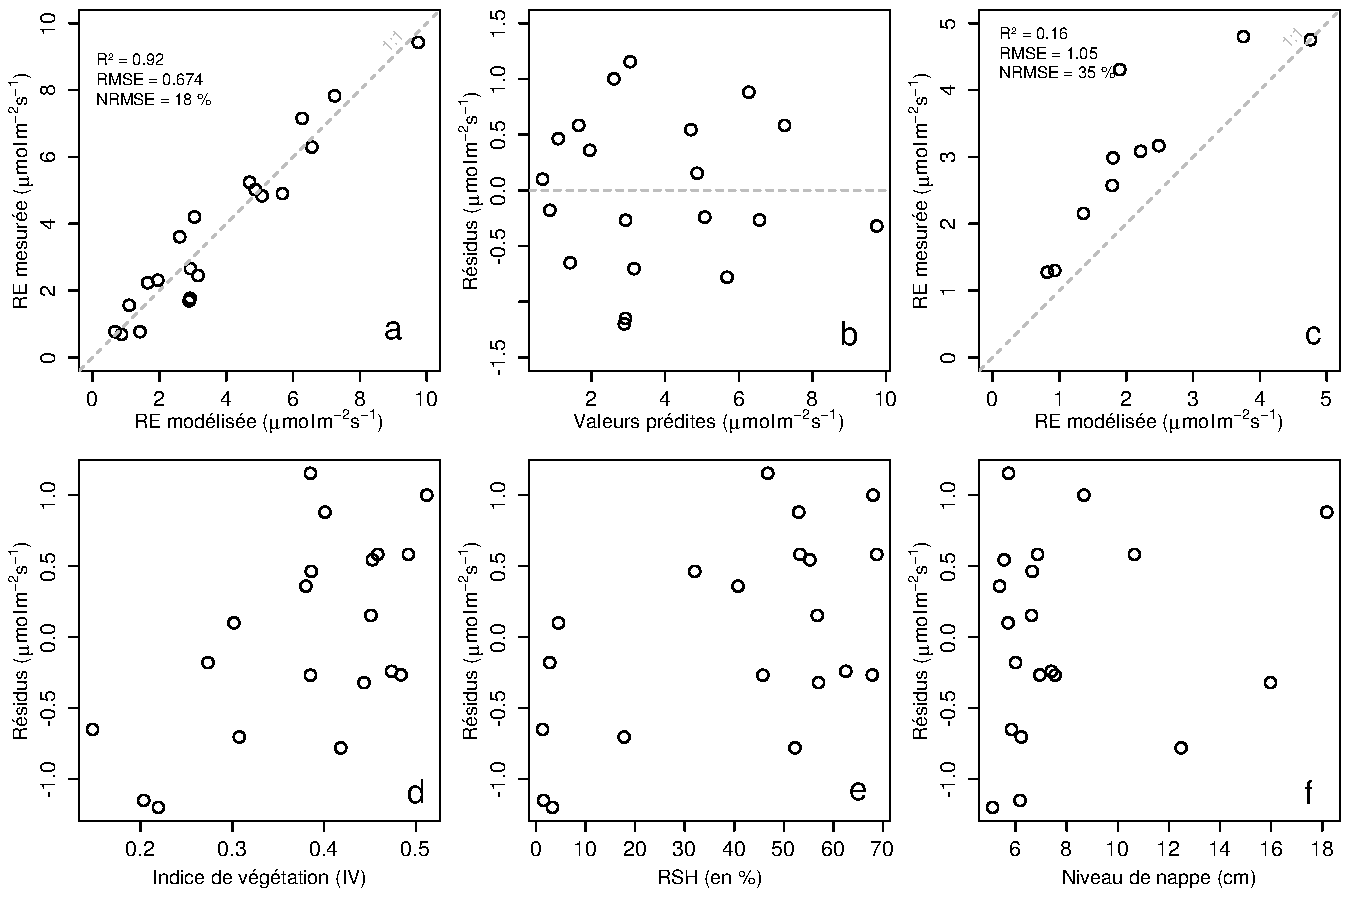
\includegraphics[width=1.05\textwidth, center]{chap3/mdl_ER_Tair}
%\caption{RE modèles avec Tair}
%\label{fig:mdl_ER_Tair}
%\end{figure}
%
%\begin{figure}
%\centering
%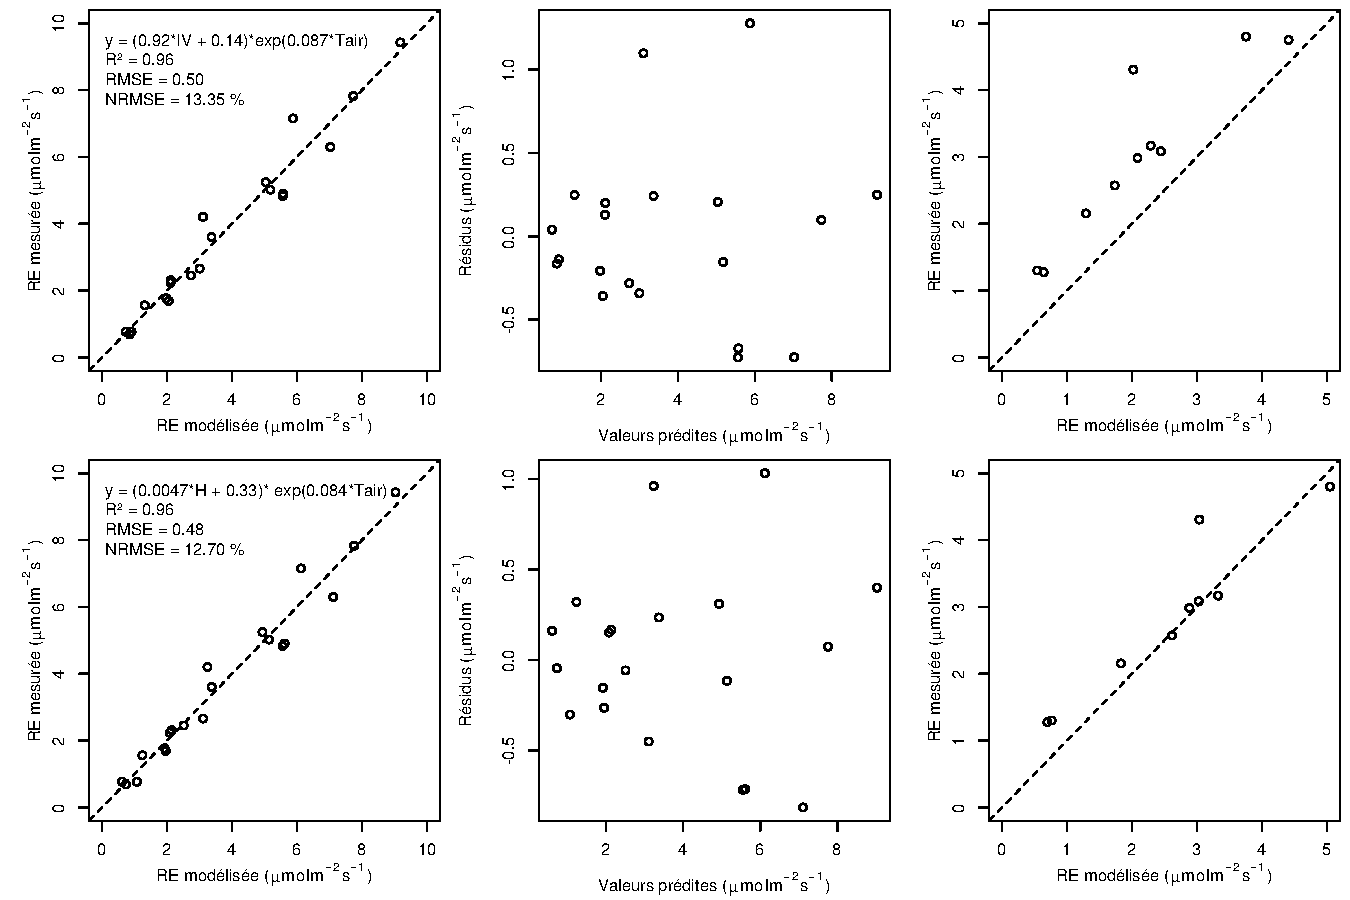
\includegraphics[width=1.05\textwidth, center]{chap3/mdl_ER_Tair_IVH}
%\caption{RE modèles avec Tair}
%\label{fig:ER_mdl_TairIVH}
%\end{figure}

%%%%%%%%%%%%%%%%%%%%% ENE
%\subsubsection{L'Échange Net de l'Écosystème}
%
%\begin{figure}
%\centering
%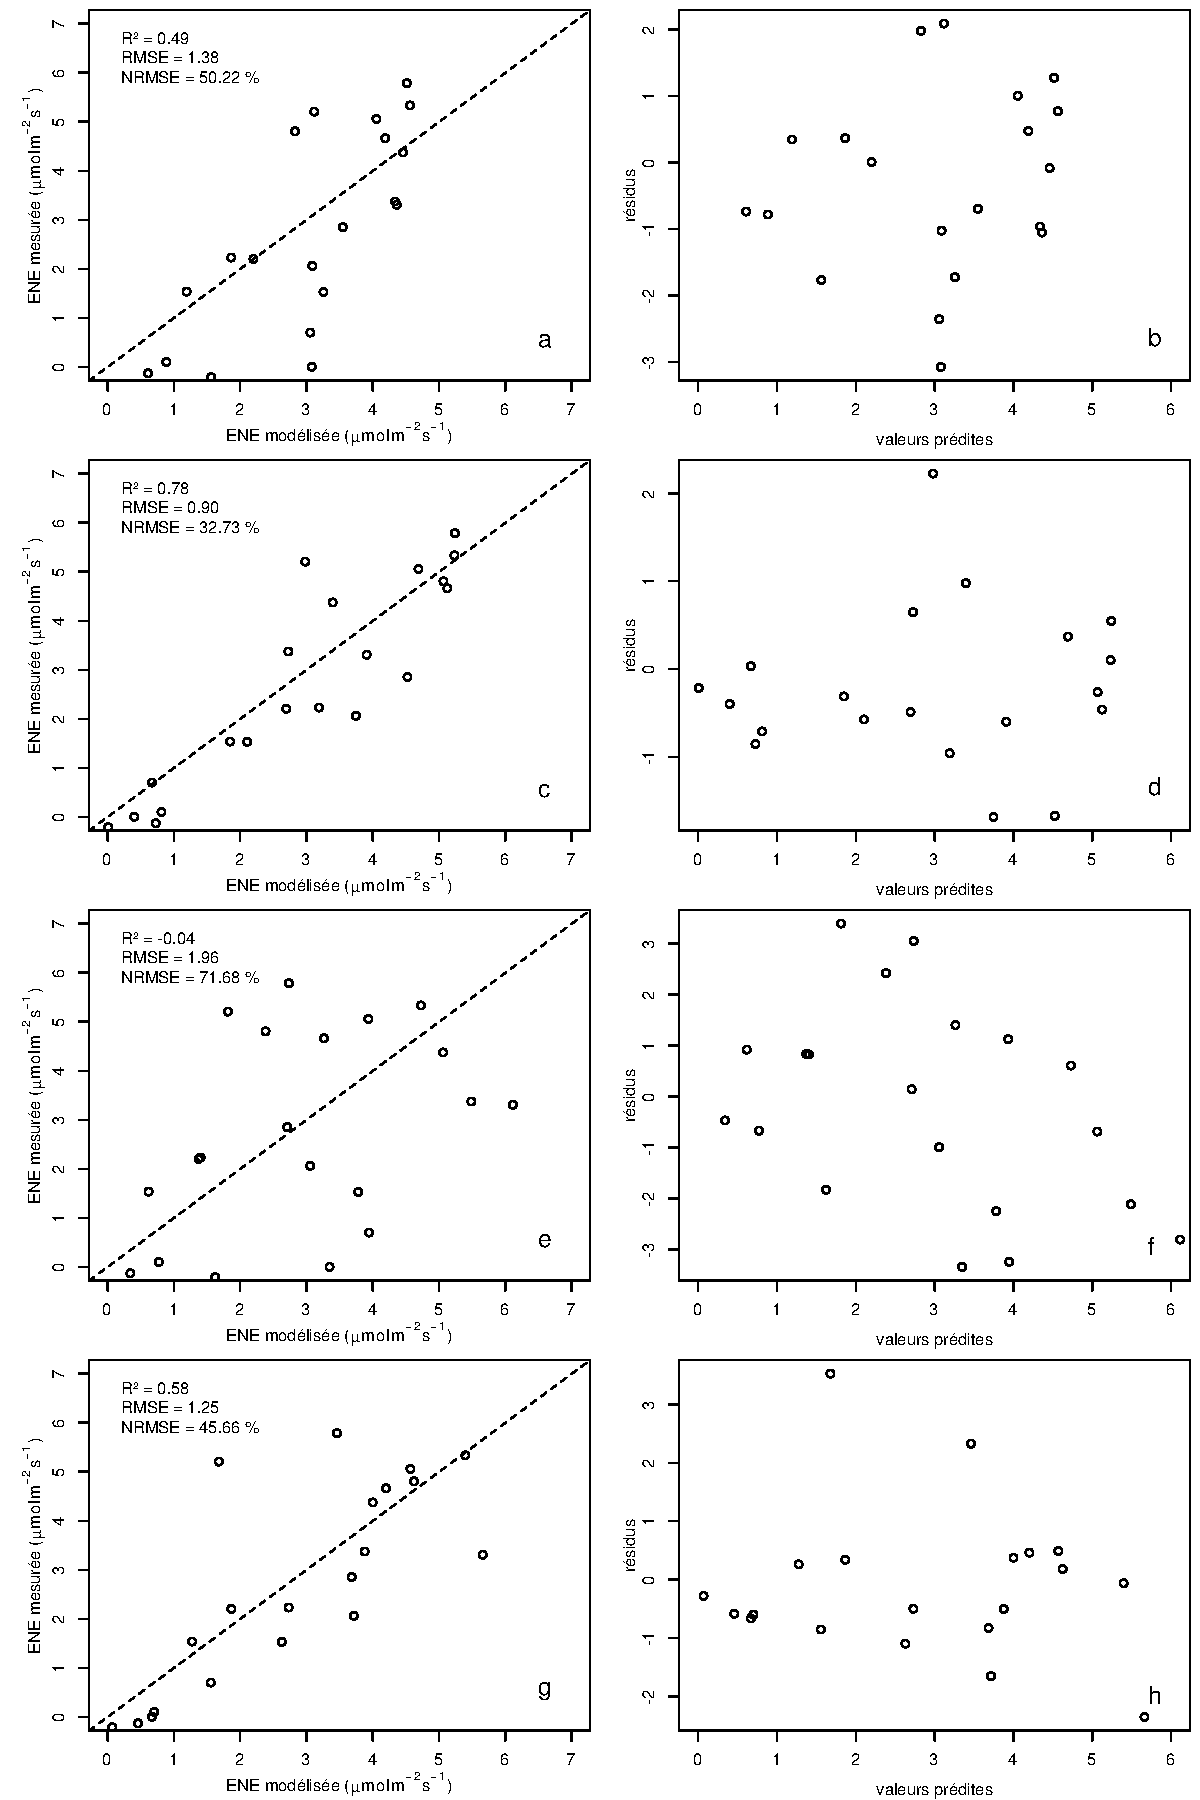
\includegraphics[width=\textwidth]{chap3/NEE_mdl_mesmod}
%\caption{ENE modèle T5 IV}
%\label{fig:ENE_mdl}
%\end{figure}
%
%L'ENE est ensuite modélisé en utilisant l'équation suivante :
%
%\begin{equation}
%ENE = PBB-RE
%\end{equation}
%
%Le résultat de cette équation (Figure~\ref{fig:ENE_mdl}), montre que ce modèle permet d'expliquer une grande partie des variations de l'ENE.
%Les résidus de cette équation sont répartis de manière a peu près homogène.

\subsubsection{Flux de \chh}

\begin{wrapfigure}{r}[35pt]{0.55\textwidth}
\centering
\vspace{-40pt}
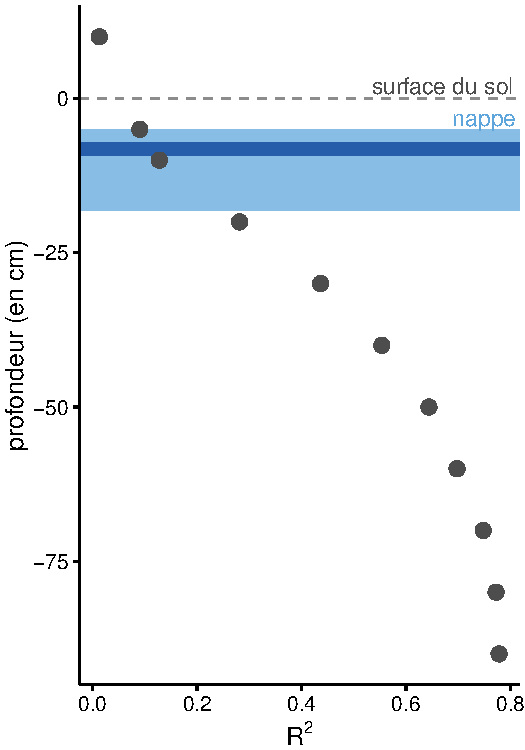
\includegraphics[width=.5\textwidth]{chap3/CH4_T_exp}
\caption{Évolution du R\textsuperscript{2} de l'équation $F_{CH_{4}} = a\times exp(b\times Temp\acute{e}rature)$ avec la profondeur. La ligne de tirets gris représente la surface du sol. La zone bleu claire représente la gamme des niveau moyen relevés sur le site et la zone bleu foncé le niveau moyen pour l'année 2013 et 2014.}
\label{fig:CH4_T}
\end{wrapfigure}

%\begin{figure}
%\centering
%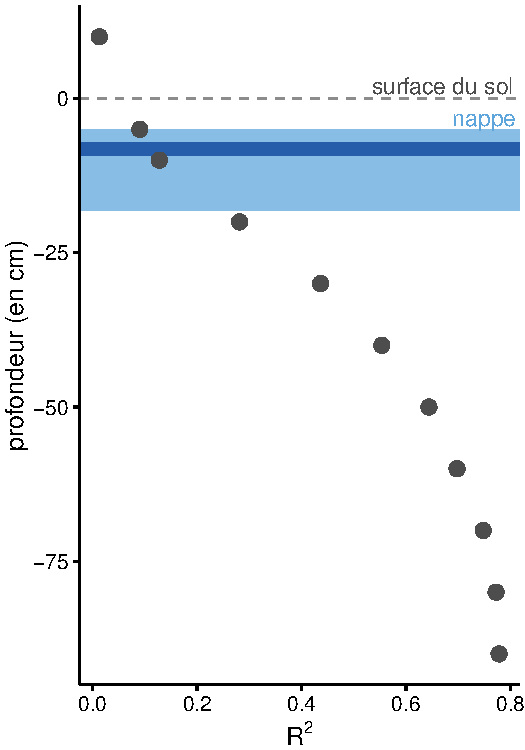
\includegraphics[width=.5\textwidth, center]{chap3/CH4_T_exp}
%\caption{Évolution du R\textsuperscript{2} de l'équation $F_{CH_{4}} = a*exp(b*Temp\acute{e}rature)$ avec la profondeur. La ligne de tirets gris représente la surface du sol. La zone bleu claire représente la gamme des niveau moyen relevés sur le site et la zone bleu foncé le niveau moyen pour l'année 2013 et 2014.}
%\label{fig:CH4_T}
%\end{figure}

Les relations entre les facteurs contrôlant mesurés et les flux de \chh sont moins claires que celles concernant le \coo.
La corrélation la plus importante est liée à la végétation (Figure~\ref{fig:Fl_FC}).
Les flux de \chh ne montre pas de tendance à augmenter de façon exponentielle avec la température de l'air.
Cependant cette relation se renforce d'autant plus que l'on utilise des températures mesurées à forte profondeur (Figure~\ref{fig:CH4_T}).
Souvent utilisée les températures proches du niveau de nappe on des R\textsuperscript{2} inférieur à \num{0.50}.
Au delà, les R\textsuperscript{2} sont supérieurs à \num{0.50}, mais l'ensemble des placettes n'est plus représenté, certaines placettes n'ayant pas une épaisseur de tourbe supérieure ou égale à \SI{30}{\centi\metre}.
Le \chh ne montre pas de relation particulière avec le niveau de la nappe.
%le \chh est également corrélé avec les températures, faiblement avec les températures de surface, mais de manière plus importante avec les températures du sol à plus forte profondeur (R\textsuperscript{2} = \textbf{XX},Figure~\ref{fig:Fl_FC}).
%Enfin il est anti-corrélé (R=-0.51) avec le niveau de la nappe.
%Les relations \chh et végétation ont donc été modélisées avec :
Les relations entre les flux de \chh et la végétation étant les plus significatives, elles ont été modélisées avec l'équation suivante :

\begin{equation} \label{eq:CH4_H}
F_{CH_{4}} = a*exp(b*IV)
\end{equation}

Avec les données acquises, l'indice de végétation est le meilleur prédicteur (Figure~\ref{fig:CH4_mdl}), car il explique \SI{78}{\percent} de la variabilité des flux \chh avec une NRMSE de \SI{32}{\percent} (Figure~\ref{fig:CH4_mdl}--a).
Aucune tendance ne semble se dégager entre les résidus de cette équation et les facteurs contrôlant mesurés (Figure~\ref{fig:CH4_mdl}--d,e,f).

L'évaluation de cette équation montre une tendance à sous-estimer les flux de \chh et une NRMSE qui double par rapport à la phase de calibration en atteignant \SI{68}{\percent} (Figure~\ref{fig:CH4_mdl}--c).
Les détails de l'estimation des paramètres de l'équation~\ref{eq:CH4_H} est visible dans le tableau~\ref{table:mdl_par} sous le nom FCH4.

\begin{figure}
\centering
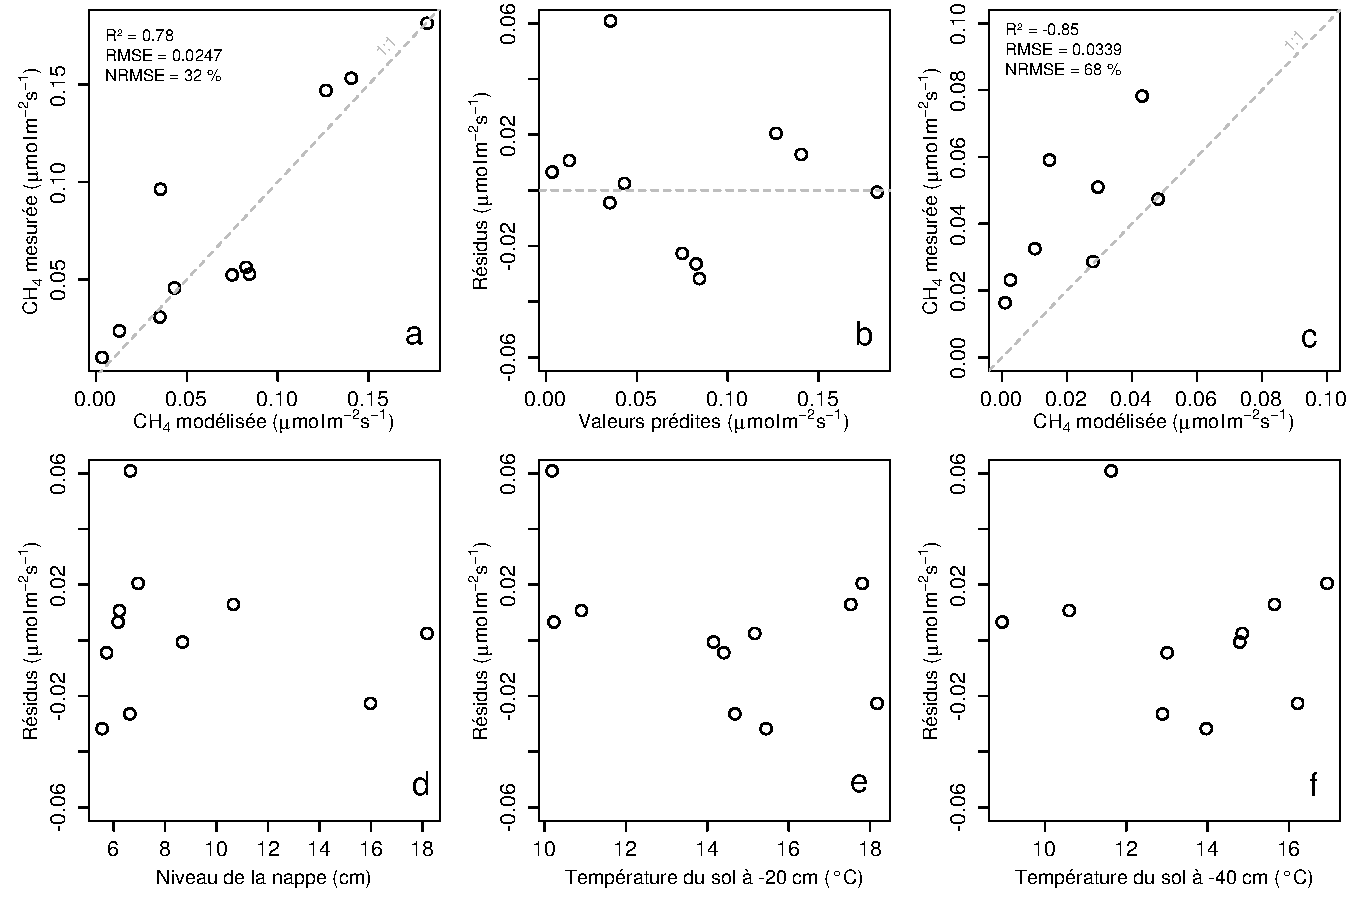
\includegraphics[width=1.15\textwidth, center]{chap3/mdl_CH4_IV}
\caption{Calibration des flux de \chh avec la végétation en utilisant l'équation~\ref{eq:CH4_H}. Avec la représentativité des modèles et la distribution des résidus de l'équation (graphes a et b), l'évaluation sur un jeu de données indépendant (graphe c) et les tendances des résidus de l'équation avec le niveau de la nappe la température du sol à \num{-20} et \SI{-40}{\centi\metre} (graphe d, e et f).}
\label{fig:CH4_mdl}
\end{figure}
%bortoluzzi veg
%Alm 1999 T -30 cm
%Bellisario relation inverse avec WTL (increased flux with lower WTL) T10
%Bubier 1993a WTL majeur
%Bubier 1995 Température humidité végétation




\subsection{Le bilan de carbone à l'échelle de l'écosystème}

%\subsubsection{Bilan (param et valeur)}

\begin{figure}[!hbt]
\centering
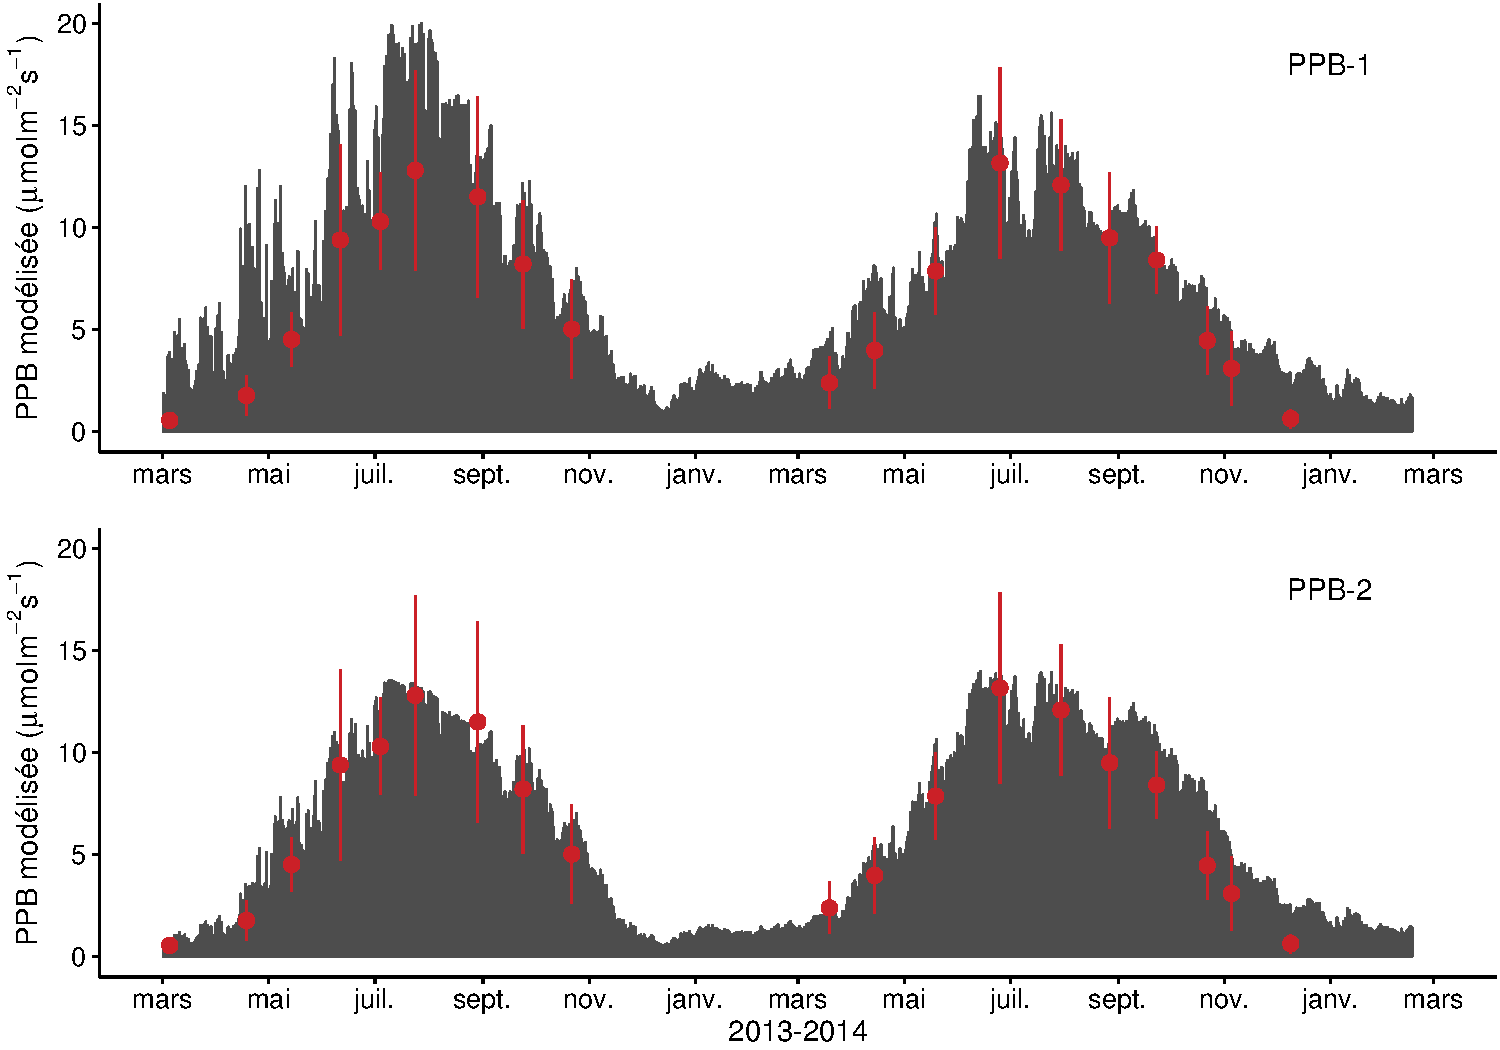
\includegraphics[width=1\textwidth, center]{chap3/BdC_GPP_interp}
\caption{Flux de \coo interpolé à l'heure à partir de PPB-1 (en haut) et PPB-2 (en bas). Les points rouges représentent les moyennes des mesures mensuelles et leur déviation standard}
\label{fig:BdC_GPP_interp}
\end{figure}

\begin{figure}
\centering
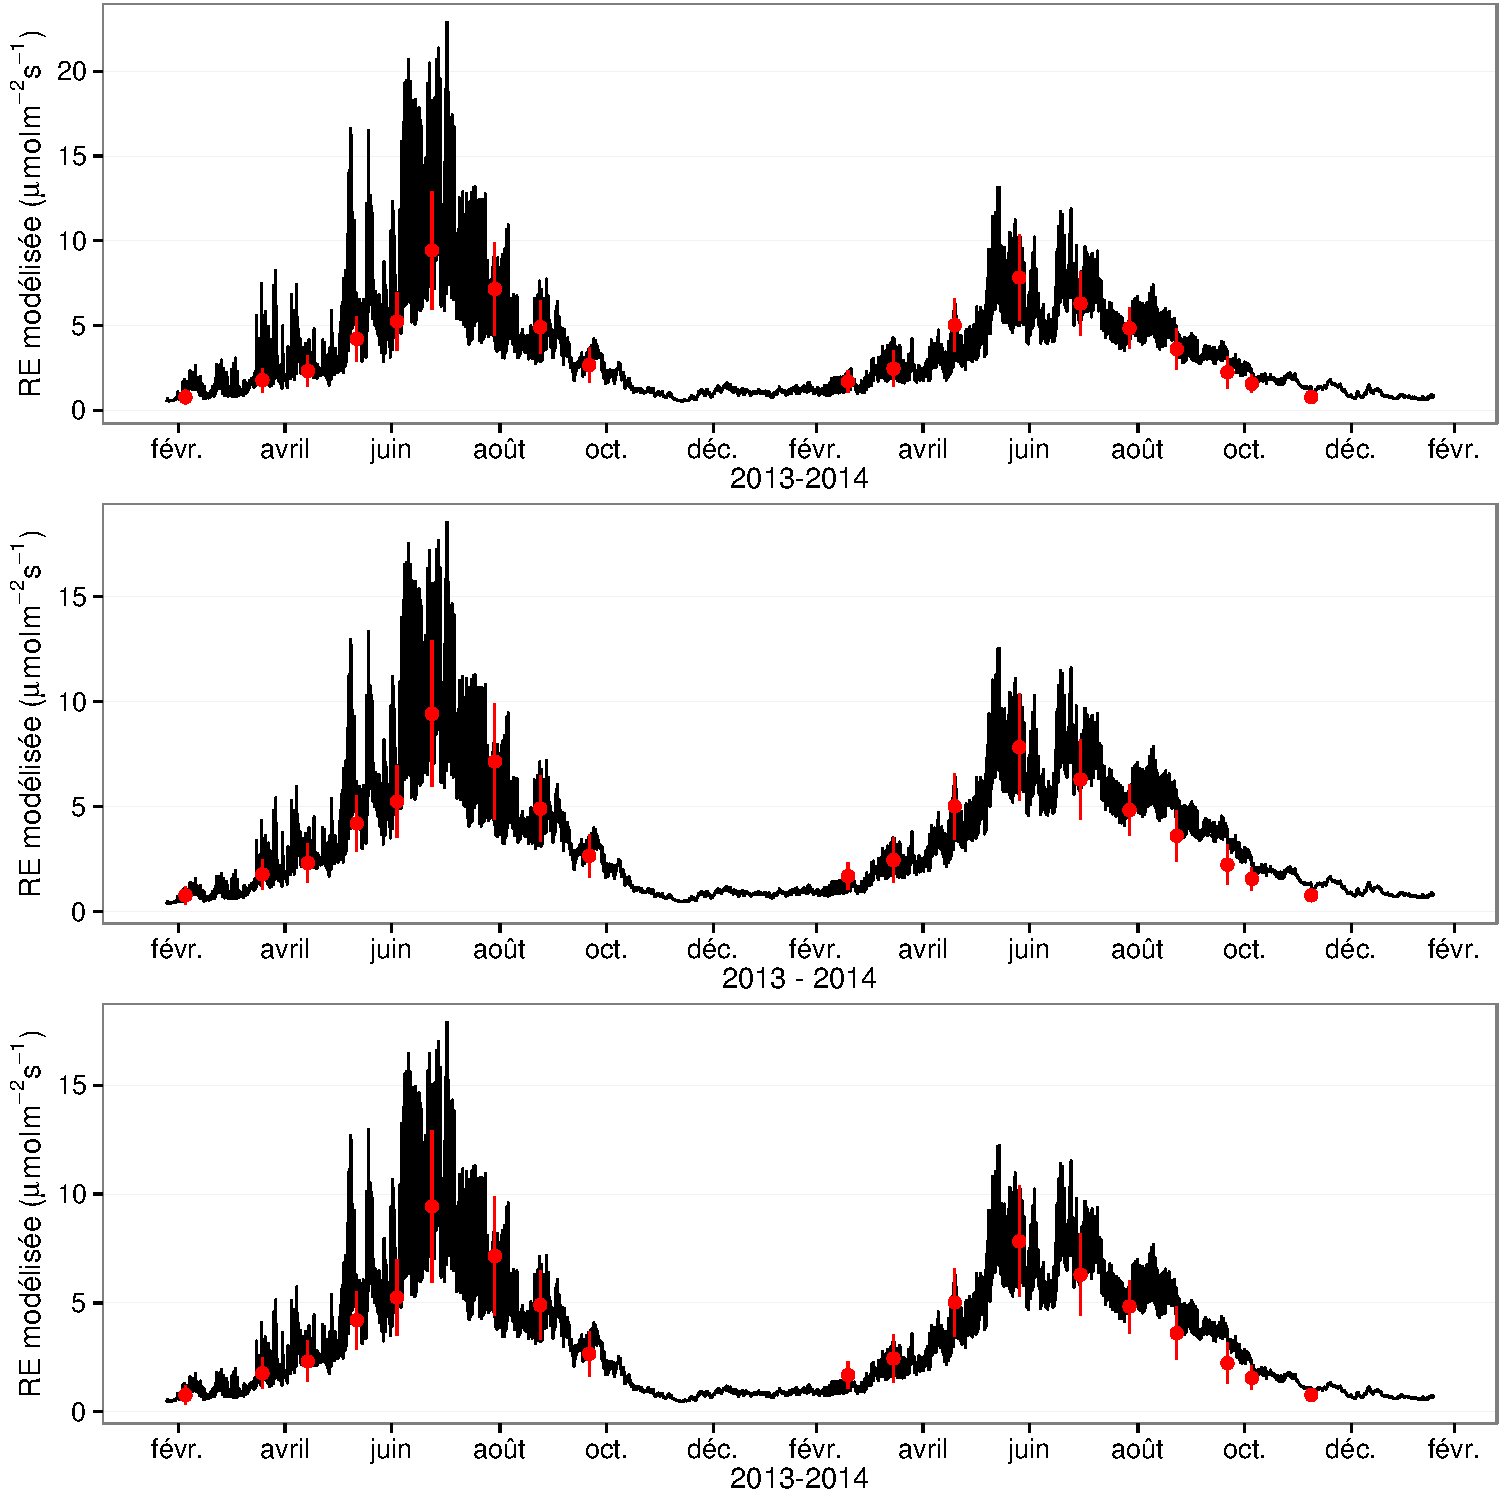
\includegraphics[width=1\textwidth, center]{chap3/BdC_ER_interp}
\caption{Flux de \coo interpolé à l'heure à partir de RE-1 (en haut), RE-2 (au milieu) et RE-3 (en bas). Les points rouges représentent les moyennes des mesures mensuelles et leur déviation standard}
\label{fig:BdC_ER_interp}
\end{figure}

\begin{figure}
\centering
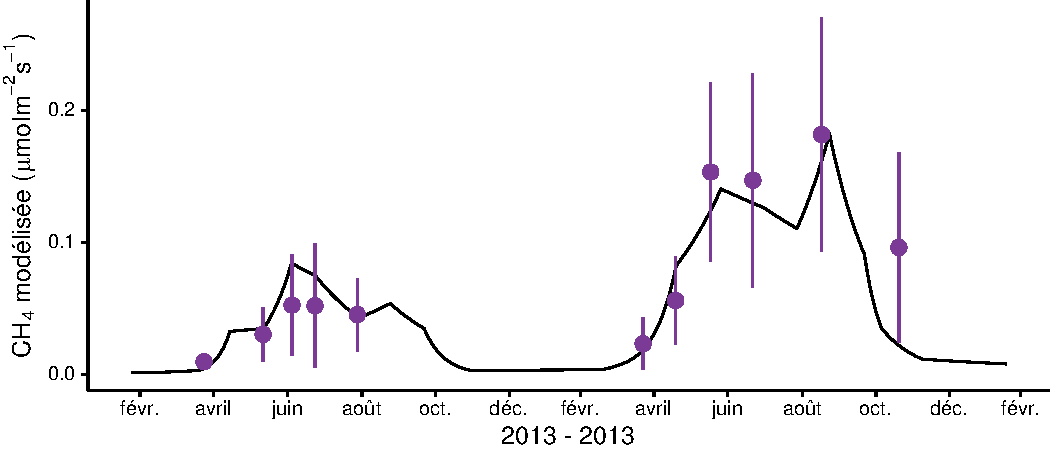
\includegraphics[width=1\textwidth, center]{chap3/CH4_BdCitp_IVcov}
\caption{Flux de \coo interpolé à partir de FCH4. Les points rouges représentent les moyennes des mesures mensuelles et leur déviation standard}
\label{fig:BdC_CH4_interp}
\end{figure}



Les interpolations des flux de PPB montrent une variabilité saisonnière proche de celle mesurée sur le terrain (Figure~\ref{fig:BdC_GPP_interp}). 
%Les valeurs mesurées les plus grandes (partie supérieure de la barre rouge sur la figure~\ref{fig:BdC_GPP_interp}) ne semblent pas être reproduite par le modèle PPB-2 à l'inverse du modèle PPB-1 (courbes noires sur la figure~\ref{fig:BdC_GPP_interp}).
Les surface grise présentes sur la figure~\ref{fig:BdC_GPP_interp} sont liées au fait que la PPB tombe à zéro toutes les nuits.
Globalement le modèle PPB-2 semble mieux représenter les moyennes des flux mesurés sur le site.
Dans les deux cas les modèles semblent sur-estimer la valeur de PPB mesurées fin 2014 et sous-estimer la PPB en été (en 2013 principalement pour PPB-1 et les 2 années pour PPB-2).

Pour la RE, l'interpolation reproduit également les variations saisonnières mesurées (Figure~\ref{fig:BdC_ER_interp}).
Les gammes de valeurs mesurées sont très proche des gammes interpolées :
les valeurs interpolées fluctuent dans les limites des barres d'erreurs.
L'interpolation des flux de la RE est très proches quel que soit le modèle utilisé (Figure~\ref{fig:BdC_ER_interp}).
L'intégration de la végétation dans les modèles RE-2 et RE-3 diminue les valeurs maximum de la RE modélisée en 2013 par rapport au modèle RE-1.

Les flux de \chh interpolés (Figure~\ref{fig:BdC_CH4_interp}), suivent également une cyclicité saisonnière.
Dans l'ensemble l'estimation du \chh semble rendre compte de la différence de flux mesuré en 2013 et en 2014.

La différence sur les cumuls quand les modèles de RE utilisent ou non la végétation est moindre : environ \SI{26}{\gcma} (tableau~\ref{table:bdc}).

\begin{table}
\centering
\caption{Cumul annuel des flux, en \si{\gcma}, en fonction des modèles utilisés.}
\label{table:flux}
\begin{tabular}{llllll}\toprule
ID & Flux & équation & 2013 & 2014 & moyen \\ \midrule
PPB-1 & PPB & \ref{eq:juneTair} et \ref{eq:PPB_bubier} & 1322 $\pm$ 410 & 1258 $\pm$ 390 & 1290 $\pm$ 400 \\
PPB-2 & & \ref{eq:juneTairIV} et \ref{eq:PPB_bubier} & 957 $\pm$ 182 & 1184 $\pm$ 225 & 1070 $\pm$ 203 \\[+1.5ex]
RE-1 & RE & \ref{eq:RE_T} & 1337 $\pm$ 241 & 1235 $\pm$ 222 & 1286 $\pm$ 231 \\
RE-2 & & \ref{eq:RE_TIV} & 1232 $\pm$ 160 & 1310 $\pm$ 170 & 1271 $\pm$ 165\\
RE-3 & & \ref{eq:RE_TH} & 1240 $\pm$ 161 & 1281 $\pm$ 167 & 1261 $\pm$ 164 \\[+1.5ex]
FCH4 & CH4 & \ref{eq:CH4_H} & 10 $\pm$ 3 & 24 $\pm$ 8 & 17 $\pm$ 5 \\[+1.5ex]
FCOD & COD & \ref{eq:COD} & 8 $\pm$ 1  & 16 $\pm$ 1 & 12 $\pm$ 1 \\
\bottomrule
\end{tabular}
\end{table}


\begin{table}
\centering
\caption{Bilan de carbone annuel, en \si{\gcma}, en fonction des modèles utilisés. Les valeurs entre parenthèses représentent l'erreur associée au bilan}
\label{table:bdc}
\begin{tabular}{llll}\toprule
combinaison de modèles & 2013 & 2014 & moyen \\ \midrule
PPB-1, RE-1, FCH4 &  \num{-33(6)} & \num{-18(0)} & \num{-26(4)} \\
PPB-1, RE-3, FCH4 &  +\num{64(16)} & \num{-64(11)} & +\num{0(3)} \\
PPB-2, RE-1, FCH4 &  \num{-398(70)} & \num{-91(14)} & \num{-245(44)} \\
PPB-2, RE-3, FCH4 &  \num{-301(47)} & \num{-138(20)} & \num{-220(33)} \\
\bottomrule
\end{tabular}
\end{table}

Les flux interpolés à une fréquence horaire puis sommés par année sont présentés dans le tableau~\ref{table:flux} pour les différents modèles utilisés.
Sur les deux années, selon le modèle utilisé, le flux total entrant via la PPB est estimé à 1070 et \SI{1290}{\gcma} pour PPB-2 et PPB-1 respectivement.
On observe une différence entre les deux modèles : 
celui utilisant uniquement la température de l'air (PPB-1) présente un stockage plus important en 2013 qu'en 2014, tandis que le modèle prenant en compte la végétation (PPB-2) stocke moins de carbone en 2013 qu'en 2014.
L'intégration de la végétation minimise également l'incertitude de l'estimation, la divisant approximativement par deux.

L'intégration de la végétation change également la différence entre 2013 et 2014 de la RE.
Lorsque la végétation est intégrée (RE-2 et RE-3) la RE est supérieure en 2014.
Lorsqu'elle ne l'est pas elle est supérieure en 2013.
Ces différences restent inférieures à l'incertitude liée aux flux estimés et on observe une grande proximité dans les valeurs des flux interpolés sur les 2 années, quel  que soit le modèle, avec un écart maximum de \SI{25}{\gcma}.

%La différence de comportement, entre les années de mesures, liée à l'intégration de la végétation est également visible dans l'estimation de la RE.
%La prise en compte de la végétation (modèles RE-2 et RE-3) conduit à une respiration plus forte en 2014 qu'en 2013 à l'inverse de RE-1.
%La différence entre l'estimation de la RE en 2013 et en 2014 diminue avec l'intégration de la végétation.
%Elle passe de 102 pour RE-1 à 78 puis 41 pour RE-2 et RE-3.
%Malgré ces différences, on observe une grande proximité dans les valeurs des flux interpolés sur les 2 années, quel  que soit le modèle, avec un écart maximum de \SI{25}{\gcma}.

Les flux de \chh estimés ont une erreur importante et sont beaucoup plus faibles que les flux de la PPB ou de la RE.
Le flux de \chh est au moins deux fois plus important en 2014 qu'en 2013.
%On y observe malgré tout un flux qui fait plus que doubler en 2014 par rapport à 2013.

Les bilans issus des différentes combinaisons de modèles (à l'exception de RE-2, non présenté car très proche de RE-3) varient de \SI{-245(44)}{\gcma} à \SI{0(3)}{\gcma} stocké dans la tourbière (Tableau~\ref{table:bdc}).
L'intégration de la végétation dans la modélisation de PPB fait baisser les bilans de carbone dans le négatif (système source) au-delà de \SI{-200}{\gcma}, avec une différence entre les bilans de \SI{220}{\gcma} environ.




\subsubsection{Carbone organique dissout}

La quantité de COD sortant de la tourbière est estimée à \SI{8}{\gcma} en 2013 et \SI{16}{\gcma} en 2014 (Tableau~\ref{table:flux}).
Les concentrations moyennes en COD mesurées à l'exutoire sont très proche pour les deux années \num{18.6} et \SI{18.3}{\mgl} respectivement.
Par contre la quantité d'eau sortant de l'écosystème est plus importante en 2014 avec un export aux alentours de \SI{1000}{\cubic\metre} par jour entre octobre 2014 et février 2015 (Figure~\ref{fig:discharge}).

\begin{figure}
\centering
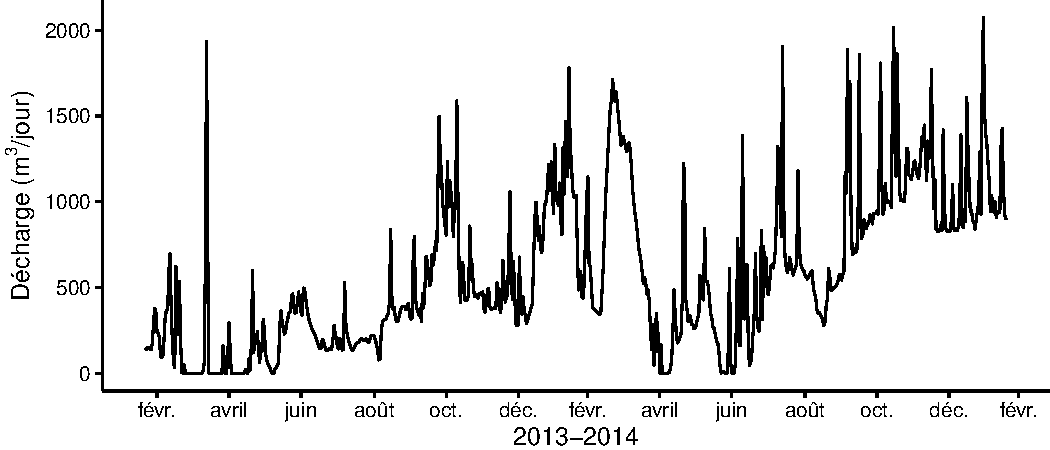
\includegraphics[width=1\textwidth, center]{chap3/discharge}
\caption{Quantité d'eau quittant le bassin versant de la tourbière, modifié d'après \citet{binet2013}.}
\label{fig:discharge}
\end{figure}


%\subsubsection{Évaluation du bilan}
%
%%\subsubsection{sensibilité des paramètres}
%\begin{table}
%\centering
%\caption{Sensibilité relative (en \%) du bilan de \coo (ENE) en réponse à une variation de $\pm$\SI{10}{\percent} de chacun des paramètres des modèles.}
%\label{table:mdl_sensitiv_BdC}
%\begin{tabular}{cccccccccc}\toprule
%& \multicolumn{3}{l}{PPB} & \multicolumn{3}{l}{RE} & \multicolumn{3}{l}{\chh} \\ 
%& & \SI{-10}{\percent} & +\SI{+10}{\percent} & & \SI{-10}{\percent} & +\SI{+10}{\percent} & & \SI{-10}{\percent} & +\SI{+10}{\percent} \\ \midrule
%& \multicolumn{3}{l}{PPB-1} & \multicolumn{3}{l}{RE-1} & \multicolumn{3}{l}{FCH4} \\ [+.5ex]
%& a & \num{-3263} & +\num{3243} & a & +\num{3371} & \num{-3371} & a & +\num{0.05} & \num{-0.05}\\
%& b & +\num{14788} & \num{-11859} & b & +\num{7616} & \num{-10078} & b & +\num{0.2} & \num{-0.36}\\
%& c & \num{-7597} & +\num{7398} & & & & & &\\
%& i & +\num{119} & \num{-139} & & & & & &\\[+1ex]
%
%& \multicolumn{3}{l}{PPB-2} & \multicolumn{3}{l}{RE-1} & \multicolumn{3}{l}{FCH4} \\ [+.5ex]
%& a & +\num{59} & \num{-57} & a & \num{-60} & +\num{60} & a & \num{0} & \num{0}\\
%& b & \num{-78} & +\num{85} & b & \num{-135} & +\num{178} & b & \num{0} & +\num{0.01}\\
%& c & +\num{40} & \num{-33} & & & & & &\\
%& d & \num{-14} & +\num{14} & & & & & &\\
%& i & \num{6.22} & \num{-5.40} & & & & & &\\[+1ex]
%
%& \multicolumn{3}{l}{PPB-1} & \multicolumn{3}{l}{RE-3} & \multicolumn{3}{l}{FCH4} \\ [+.5ex]
%& a & \num{-426} & +\num{423} & a & +\num{168} & \num{-168} & a & +\num{0.01} & \num{-0.01}\\
%& b & +\num{1931} & \num{-1548} & b & +\num{813} & \num{-1018} & b & +\num{0.03} & \num{-0.05}\\
%& c & \num{-992} & +\num{966} & c & +\num{263} & \num{-263} & & &\\
%& i & \num{-18} & +\num{15} & & & & & &\\[+1ex]
%
%& \multicolumn{3}{l}{PPB-2} & \multicolumn{3}{l}{RE-3} & \multicolumn{3}{l}{FCH4} \\ [+.5ex]
%& a & +\num{67} & \num{-65} & a & \num{-26} & +\num{26} & a & 0 & 0\\
%& b & \num{-89} & +\num{97} & b & \num{-125} & +\num{157} & b & 0 & 0\\
%& c & +\num{45} & \num{-38} & c & \num{-40} & +\num{40} & & &\\
%& d & \num{-16} & +\num{16} & & & & & &\\
%& i & +\num{7.1} & \num{-6.1} & & & & & &\\[+1ex]
%
%\bottomrule
%\end{tabular}
%\end{table}
%
%L'analyse de sensibilité, consistant à faire varier chaque paramètre des modèles de $\pm$\SI{10}{\percent}, les combinaisons de modèles PPB-1, PPB-2, RE-1 et RE-3 ont été testé (Tableau~\ref{table:mdl_sensitiv_BdC}).
%Le modèle RE-2, très proche du modèle RE-3 n'a pas été testé.
%\textbf{Attente du COD, les valeurs du tableau sont fausse pour le moment}


\subsubsection{Représentativité locale du bilan de \coo}

En recalculant des valeurs de NRMSE individuelles pour chaque placette, il est possible d'avoir une indication sur la représentativité locale des modèles calibrés à l'échelle de l'écosystème (Figure~\ref{fig:repr_loc}).
Que ce soit pour la PPB ou la RE, la placette n°5 a systématiquement une NRMSE significativement plus élevée que les autres.

Pour la PPB et si l'on excepte la placette n°5, les estimations à l'échelle de l'écosystème permettent de représenter les placettes avec une NRMSE comprise entre 20 et \SI{90}{\percent} pour PPB-1 et entre 30 et \SI{100}{\percent} pour PPB-2.
PPB-1 et PPB-2 ont une distribution des valeurs de NRMSE relativement similaire.

La NRMSE de RE-1 est comprise entre 20 et \SI{100}{\percent}, celle de RE-3 entre 20 et \SI{80}{\percent}.
La majorité des placettes ont une NRMSE d'environ \SI{55}{\percent} pour RE-1 et d'environ \SI{40}{\percent} pour RE-3 (Figure~\ref{fig:repr_loc}).
le modèle RE-3 a des valeurs plus faibles et une distribution plus homogène de la NRMSE que RE-1, avec davantage de placette en dessous de \SI{50}{\percent} (12 contre 8).

\begin{figure}
\centering
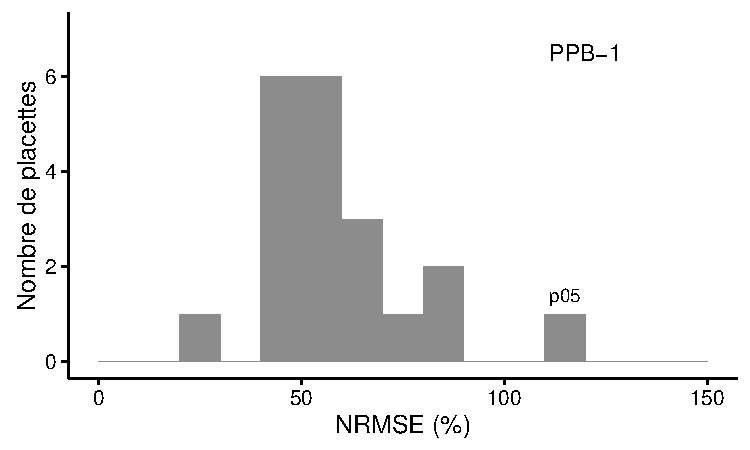
\includegraphics[width=.45\textwidth]{chap3/eco_to_loc_nrmse_PPB1}
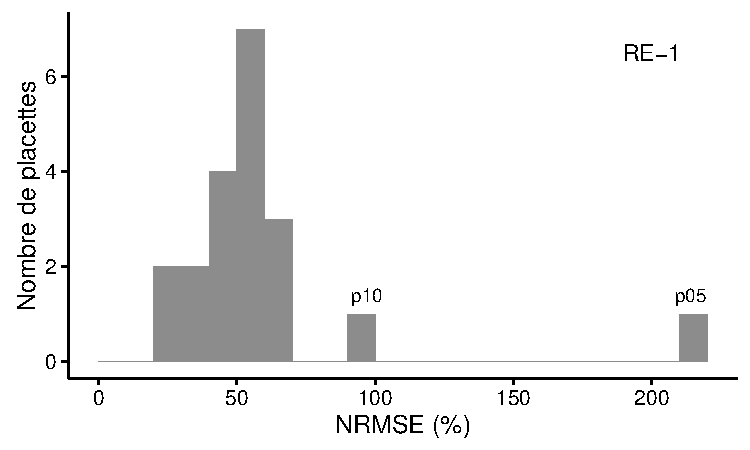
\includegraphics[width=.45\textwidth]{chap3/eco_to_loc_nrmse_RE1}\\
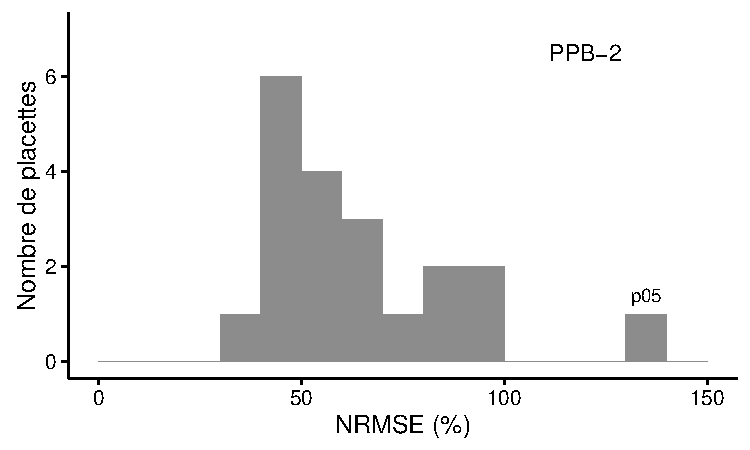
\includegraphics[width=.45\textwidth]{chap3/eco_to_loc_nrmse_PPB2}
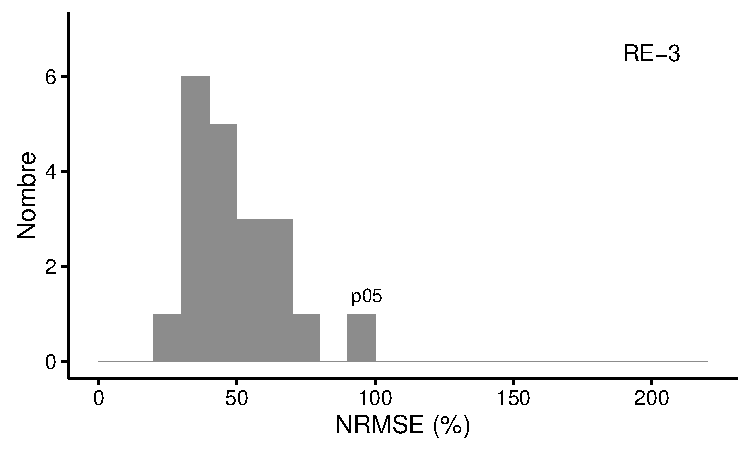
\includegraphics[width=.45\textwidth]{chap3/eco_to_loc_nrmse_RE3}
\caption{Distribution des valeurs de la NRMSE recalculée par placette à partir des modèles calibrés à l'échelle de l'écosystème}
\label{fig:repr_loc}
\end{figure}



%, montre pour une équation exponentielle simple des valeurs attendues $\pm$\SI{10}{\percent} pour le paramètre a et \num{+29} à \SI{-22}{\percent} pour le b (Figure~\ref{table:mdl_sensitiv}).
%Pour la PPB issue des équations~\ref{eq:juneTairIV} et \ref{eq:PPB_bubier} le paramètre i à très peu d'effet sur le bilan, \num{0} à \SI{-1}{\percent}.
%Cependant l'effet sur le bilan augmente lorsque la végétation est prise en compte (équation~\ref{eq:juneTair} et \ref{eq:PPB_bubier}) : \num{-8} à \SI{-10}{\percent}.
%À l'inverse, la sensibilité de l'ensemble des autres paramètres (a, b, c) diminue lorsque l'indice de végétation est pris en compte.
%Le paramètre a est l'exception, passant de \num{-10} à \SI{-17}{\percent} pour une baisse de \SI{10}{\percent}.
%Considérant le modèle de PPB prenant en compte la végétation, la sensibilité maximum des différents paramètres du bilan est proche de \SI{30}{\percent}, et similaire pour la PPB et la RE.



%\begin{table}
%\centering
%\caption{Sensibilité relative (en \%) du bilan de \coo (ENE) en réponse à une variation de $\pm$\SI{10}{\percent} de chacun des paramètres des modèles.}
%\label{table:mdl_sensitiv_BdC}
%\begin{tabular}{llccccccccccc}\toprule
%& \multicolumn{4}{l}{PPB} & \multicolumn{4}{l}{RE} & \multicolumn{4}{l}{\chh} \\ 
%& par & valeur & \SI{-10}{\percent} & +\SI{+10}{\percent} & par & valeur & \SI{-10}{\percent} & +\SI{+10}{\percent} & par & valeur & \SI{-10}{\percent} & +\SI{+10}{\percent} \\ \midrule
%\multicolumn{13}{l}{PPB-2, ER-3, FCH4} \\ [+.5ex]
%& a & 0.34 & -766 & 766 & a & 26.23 & 741 & -736 & a & 17.82 & -12.28 & 12.28 \\
%& b & 0.10 & -1730 & 2289 & b & 53.68 & -3358 & 2693 & b & 0.03 & -15.08 & 17.68 \\
%& c &  & & & c & 27.21 & 1725 & -1680 & & & & \\
%& d &  & & & c & 27.21 & 1725 & -1680 & & & & \\
%& e &  & & & i & 1.84 & 31.56 & -26.92 & & & & \\[+1ex]
%%\multicolumn{13}{l}{mdl 2 équation~\ref{eq:RE_T5} et équation~\ref{eq:juneTairIV} Tair, Tair IVcov, H} \\ [+.5ex]
%%& a & 0.34 & -71.08 & 71.08 & a & 33.66 & 56.25 & -55.32 & a & 17.82 & -1.14 & 1.14 \\
%%& b & 0.10 & -160.59 & 212.51 & b & 42.45 & -119.84 & 123.69 & b & 0.03 & -1.40 & 1.64 \\
%%&  &  & & & c & 25.77 & 62.63 & -53.28 & & & & \\
%%&  &  & & & i & 0.33 & 6.94 & -6.02 & & & & \\[+1ex]
%%\multicolumn{13}{l}{mdl 3 équation~\ref{eq:RE_T5IV} et équation~\ref{eq:juneTairIV} Tair IVcov, Tair IVcov, H} \\ [+.5ex]
%%& a & 0.92 & -55.69 & 55.69 & a & 33.66 & 61.31 & -60.31 & a & 17.82 & -1.24 & 1.24 \\
%%& b & 0.09 & -149.40 & 189.01 & b & 42.45 & -130.64 & 134.84 & b & 0.03 & -1.53 & 1.79 \\
%%& c & 0.14 & -20.89 & 20.89 & c & 25.77 & 68.28 & -58.08 & & & & \\
%%&  &  & & & i & 0.33 & 7.57 & -6.56 & & & & \\
%\bottomrule
%\end{tabular}
%\end{table}


%\begin{table}
%\centering
%\caption{Sensibilité relative (en \%) des flux en réponse à une variation de $\pm$\SI{10}{\percent} de chacun des paramètres des modèles.}
%\label{table:mdl_sensitiv}
%\begin{tabular}{llccccccccccc}\toprule
%& \multicolumn{4}{l}{RE} & \multicolumn{4}{l}{GPP} & \multicolumn{4}{l}{\chh} \\ 
%& par & valeur & \SI{-10}{\percent} & +\SI{+10}{\percent} & par & valeur & \SI{-10}{\percent} & +\SI{+10}{\percent} & par & valeur & \SI{-10}{\percent} & +\SI{+10}{\percent} \\ \midrule
% & \multicolumn{4}{l}{Tair} & \multicolumn{4}{l}{Tair} & \multicolumn{4}{l}{H} \\ [+.5ex]
%& a & 0.34 & -10   & 10   & a & 26.23 & -9.7 &  9.6 & a & 17.82 &-10.0 & 10.0 \\
%& b & 0.10 & -22.6 & 29.9 & b & 53.68 & 43.7 &-35.1 & b &  0.03 &-12.3 & 14.4 \\
%&   &      &       &      & c & 27.21 &-22.5 & 21.9 &   &       &      &      \\
%&   &      &       &      & i &  1.84 & -0.4 &  0.4 &   &       &      &      \\[+1ex]
% & \multicolumn{4}{l}{Tair IVcov} & \multicolumn{4}{l}{Tair IVcov} & & & & \\ [+.5ex]
%& a & 0.92 & -7.3  & 7.3 & a & 33.66 & -9.0 &  8.9 & & & & \\
%& b & 0.09 & -19.5 & 24.7& b & 42.45 & 19.3 &-19.9 & & & & \\
%& c & 0.14 & -2.7  & 2.7 & c & 25.77 &-10.1 &  8.6 & & & & \\
%&   &      &       &     & i & 0.33  & -1.1 &  1.0 & & & & \\[+1ex]
%\bottomrule
%\end{tabular}
%\end{table}




%\subsubsection{pseudo-validation et erreur}

%\begin{figure}
%\centering
%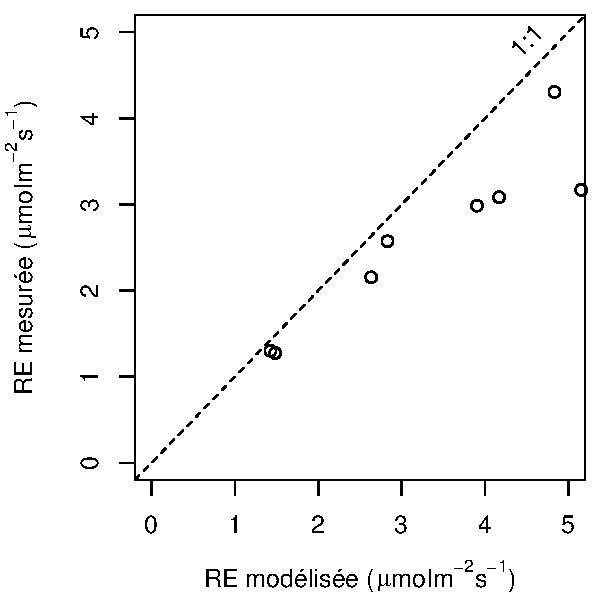
\includegraphics[width=.5\textwidth]{chap3/ER_T5_val}
%\caption{Évaluation RE}
%\label{fig:RE_T5_val}
%\end{figure}
%\begin{figure}
%\centering
%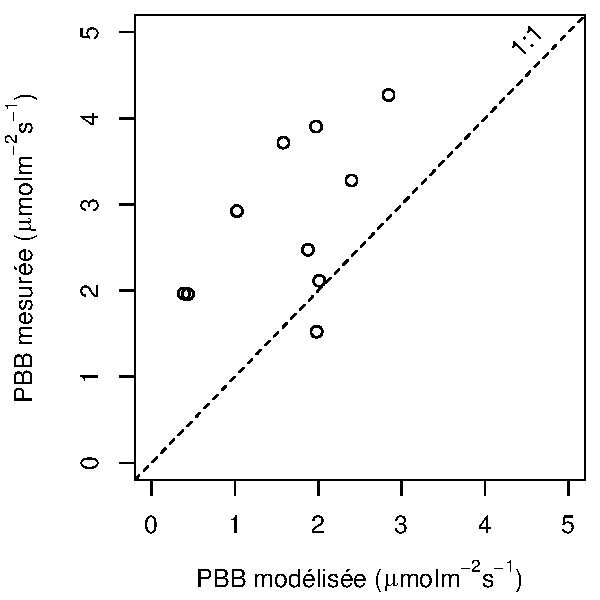
\includegraphics[width=.5\textwidth]{chap3/GPP_TairIVcov_val}
%\caption{Évaluation GPP}
%\label{fig:GPP_TairIVcov_val}
%\end{figure}

\subsection{Variabilité spatiale du bilan de \coo}

\subsubsection{Calibration par groupe de placette}



La classification hiérarchique a permis de distinguer 4 groupes de végétation (Figure~\ref{fig:tree}).
Dans le groupe Mousse, la strate muscinale est majoritaire avec un recouvrement moyen de \SI{91}{\percent}, et des recouvrements inférieurs à \num{35} et \SI{15}{\percent} pour les strates herbacées et arbustives respectivement (Figure~\ref{fig:distrib_grpveg}).
Le groupe Mix est le plus homogène avec un recouvrement moyen des strates muscinales et arbustives de \num{63} et \SI{58}{\percent}.
C'est également le groupe dans lequel il y a le moins d'herbacées (\SI{24}{\percent}).
Dans le groupe Herbe, la strate herbacée est majoritaire avec un recouvrement moyen de \SI{63}{\percent}, la strate arbustive est moins présente (\SI{19}{\percent} en moyenne) et la strate muscinale est absente ($\approx$\SI{1}{\percent}).
La strate muscinale est également absente, dans le groupe Arbuste ($\approx$\SI{1}{\percent}), dans lequel la strate herbacée à un recouvrement de \SI{33}{\percent} et la strate arbustive de \SI{65}{\percent}.

Les flux, calculés pour chaque groupe à partir des même équations que celles utilisées à l'échelle de l'écosystème entier, ont des NRMSE plus importantes : de \num{41} à \SI{66}{\percent} pour RE-1 et RE-3 et de \num{39} à \SI{65}{\percent} pour PPB-1 et PPB-2 (Tableau~\ref{table:flux_grp}).

Les flux de RE estimés en regroupant les placettes sont du même ordre de grandeur que ceux estimés pour l'ensemble de l'écosystème : entre \num{975(648)} et \SI{1453(740)}{\gcma} pour RE-1 et RE-3 (Tableau~\ref{table:flux_grp}).
Les groupes Mix et Arbuste ont des flux similaires pour les deux modèles : \num{1365(670)} et \SI{1237(582)}{\gcma} pour RE-1 et \num{1393(681)} et \SI{1274(576)}{\gcma} pour RE-3.
Ces flux sont les plus proches de ceux estimés à l'échelle de l'écosystème (\num{1286(231)} et \SI{1261(164)}{\gcma} pour RE-1 et RE-3).
La prise en compte de la végétation (RE-3) fait diminuer fortement le flux estimé pour le groupe Herbe dont la RE passe de \num{1453(740)} à \SI{1115(455)}{\gcma}.
Parmi l'ensemble des groupes, le groupe Mousse à la RE la plus faible quel que soit le modèle considéré : \num{975(648)} et \SI{1023(439)}{\gcma} respectivement pour RE-1 et RE-3.
%Pour la RE les flux sont du même ordre de grandeur que ceux calculés avec l'ensemble des placettes, que ce soit pour RE-1 ou RE-2.
%Le groupe Mousse a, pour les deux modèles, un flux annuel plus faible que le flux calculé à l'échelle de l'écosystème.
%Le groupe Arbuste est, quant à lui, le plus proche des flux « écosystèmes » tandis que le groupe Mix est au dessus.
%L'estimation de la RE du groupe Herbe est supérieure a celle estimée à l'échelle de l'écosystème pour RE-1 et inférieure pour RE-3.
%La RE du groupe Mousse est inférieur aux autres groupes que ce soit pour RE-1 ou RE-3. 
%Entre RE-1 et RE-3 les estimations du groupe Herbe diminue de façon importante (\num{-338}) alors qu'elles sont relativement similaire ($\pm$\num{50}) pour les autres groupes.

Concernant la PPB, les estimations des modèles calibrés par groupes sont inférieures à celles calculées à l'échelle de l'écosystème.
Ces relations sont à relativiser en considération des fortes incertitudes (Tableau~\ref{table:flux_grp}).
Ainsi les estimations par groupes de PPB-1 ont des valeurs comprises entre \num{886(501)} et \SI{1065(465)}{\gcma}, contre \SI{1290(400)}{\gcma} et les estimation de PPB-2 varient de \num{808(387)} à \SI{1277(642)}{\gcma}, par rapport à \SI{1070(203)}{\gcma} à l'échelle de l'écosystème.
Seul la PPB du groupe Herbe estimée avec PPB-2 est supérieure aux estimations faite pour l'ensemble des placettes.
À l'inverse de la RE, l'intégration de la végétation augmente, de \num{1056(682)} à \SI{1277(642)}{\gcma}, le flux du groupe Herbe.
En revanche, comme pour la RE, le groupe Mousse est celui dont les flux sont les plus faibles (\num{886(501)} et \SI{808(387)}{\gcma} pour PPB-1 et PPB-2).

Pour la PPB, les estimations de PPB-1 sont systématiquement inférieures à celles réalisées à l'échelle de l'écosystème.
Pour PPB-2 seul le groupe Herbe à une estimation supérieure.
Les différences entre PPB-1 et PPB-2 sont plus importantes que celles observées pour RE, même si la plus grande différence (\num{221}) est observée pour le même groupe, le groupe Herbe.
Le groupe Mix cependant une différence du même ordre de grandeur (\num{189}), tandis que pour les deux autres groupes cette différence est plus faible (78 et 58 respectivement pour les groupes Mousse et Arbuste).

\begin{figure}
\centering
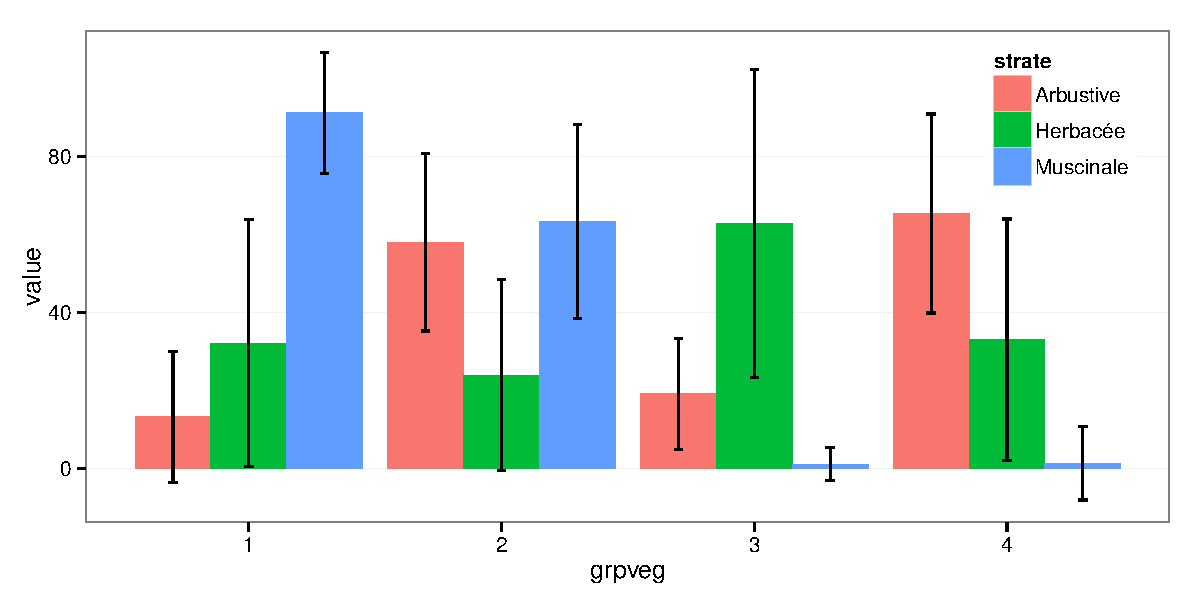
\includegraphics[width=\textwidth]{chap3/distrib_grpveg}
\caption{Recouvrement végétal moyen par strate (en \si{\percent}) des 4 groupes, les groupes sont nommés en fonction de la végétation majoritaire. Les barres d'erreur représente la déviation standard.}
\label{fig:distrib_grpveg}
\end{figure}

En terme de bilan de \coo, les groupes Arbuste et Mousse sont ceux qui sont le moins impactés par le choix des modèles (Tableau~\ref{table:bdc_grp}).
Quand la végétation n'est pas prise en compte pour l'estimation de la RE (modèle RE-1), le groupe Mousse est celui dont le bilan est le moins négatif.
Quand la végétation est prise en compte (modèle RE-3) c'est le groupe Herbe qui perd le moins de carbone (PPB-1, RE-3) voire qui en stocke (PPB-2, RE-3).
Les groupes Mix et Arbustes ont des valeurs de bilan généralement proche quand la végétation n'est pas prise en compte dans l'estimation de la PPB.
%Les bilans de \coo calculés par groupe de végétations sont présentés dans le tableau~\ref{table:bdc_grp}.
%On constante que du point de vue de l'ENE les groupes Mousse et Mix sont relativement proche, et que le groupe Arbuste est du même ordre de grandeur bien qu'avec une ENE un peu plus élevée.
%Le groupe Herbe est le seul groupe présentant une ENE positive, du même ordre de grandeur que les précédentes en valeur absolue.
%Dans le détail, la RE est la plus forte, supérieure à \SI{1200}{\gcma}, dans les groupes Mix et Arbuste.
%Elle est plus faible dans les groupes Mousse et Herbe (environ \SI{1000}{\gcma}).
%Pour la PPB, la valeur la plus faible est dans le groupe Mousse et la plus forte dans le groupe Herbe avec plus de \SI{1300}{\gcma}, soit une différence de plus de \SI{600}{\gcma}.
%Les groupes Mix et Arbuste sont relativement proches avec des valeurs intermédiaires avoisinant \SI{1000}{\gcma}.




%\begin{table}
%\centering
%\caption{Bilan des flux de \coo en \si{\gcma}, en utilisant PPB-2 et RE-3}
%\label{table:bdc_grp}
%\begin{tabular}{llll}\toprule
%groupe & PPB-2 & RE-3 & ENE \\ \midrule
%Mousse &  \num{714} & \num{1023} & \num{-308} \\
%Mix &  \num{1045} & \num{1385} & \num{-340} \\
%Herbe &  \num{1323} & \num{1057} & \num{266} \\
%Arbuste &  \num{1002} & \num{1262} & \num{-260} \\
%\bottomrule
%\end{tabular}
%\end{table}

\begin{table}
\centering
\caption{Cumul des flux de \coo en \si{\gcma} interpolés par groupe de végétation avec les modèles RE-1 et RE-3 pour la respiration et les modèles PPB-1 et PPB-2 pour la photosynthèse. (Le modèle RE-2, très proche de RE-3 n'a pas été inclus)}
\label{table:flux_grp}
\begin{tabular}{lllllll}\toprule
& \multicolumn{3}{c}{RE} &  \multicolumn{3}{c}{PPB} \\ \cmidrule(lr){2-4} \cmidrule(lr){5-7} 
groupe & valeur & R\textsuperscript{2} & NRMSE & valeur & R\textsuperscript{2} & NRMSE\\ \midrule
& \multicolumn{3}{l}{RE-1} &  \multicolumn{3}{l}{PPB-1} \\
Mousse &  \num{975} & \num{0.22} & \num{66.48} & \num{886} & \num{0.42} & \num{56.54} \\
Mix &  \num{1365} & \num{0.58} & \num{49.09} & \num{1065} & \num{0.56} & \num{43.70}  \\
Herbe &  \num{1453} & \num{0.56} & \num{50.93}  & \num{1056} & \num{0.42} & \num{64.66} \\
Arbuste &  \num{1237} & \num{0.49} & \num{47.02} & \num{895} & \num{0.31} & \num{58.86}  \\ [+1ex]
& \multicolumn{3}{l}{RE-3} &  \multicolumn{3}{l}{PPB-2} \\
Mousse &  \num{1023} & \num{0.68} & \num{42.91} & \num{808} & \num{0.58} & \num{47.92} \\
Mix &  \num{1393} & \num{0.58} & \num{48.88} & \num{876} & \num{0.65} & \num{38.93}  \\
Herbe &  \num{1115} & \num{0.72} & \num{40.84}  & \num{1277} & \num{0.65} & \num{50.30} \\
Arbuste &  \num{1274} & \num{0.53} & \num{45.25} & \num{953} & \num{0.46} & \num{52.14}  \\
\bottomrule
\end{tabular}
\end{table}

%\begin{table}
%\centering
%\caption{Bilan des flux de \coo en \si{\gcma}, en utilisant PPB-2 et RE-3}
%\label{table:bdc_grp}
%\begin{tabular}{llllll}  \cmidrule[0.08em](r){1-5}%\toprule
%année & Mousse & Mix & Herbe & Arbuste & \\ \cmidrule(r){1-5} %\midrule
%\multicolumn{6}{l}{PPB-1, RE-1} \\
%%2013 &  \num{-147} & \num{-321} & \num{-436} & \num{-368} & \num{-15}\\
%%2014 &  \num{-32} & \num{-280} & \num{-357} & \num{-314} & +\num{23} \\
%2 années &  \num{-90} & \num{-300} & \num{-397} & \num{-341} & +\num{4}\\[+1ex]
%\multicolumn{6}{l}{PPB-1, RE-3} \\
%%2013 &  \num{-136} & \num{-342} & \num{-2} & \num{-344} & +\num{82} \\
%%2014 &  \num{-139} & \num{-315} & \num{-116} & \num{-413} & \num{-23} \\
%2 années &  \num{-138} & \num{-328} & \num{-59} & \num{-378} & +\num{29} \\[+1ex]
%\multicolumn{6}{l}{PPB-2, RE-1} \\
%%2013 &  \num{-274} & \num{-596} & \num{-356} & \num{-403} & \num{-380} \\
%%2014 &  \num{-61} & \num{-383} & +\num{5} & \num{-165}& \num{-51} \\
%2 années &  \num{-168} & \num{-489} & \num{-175} & \num{-284} & \num{-216} \\[+1ex]
%\multicolumn{6}{l}{PPB-2, RE-3} \\
%%2013 &  \num{-263} & \num{-616} & +\num{79} & \num{-378} & \num{-283} \\
%%2014 &  \num{-168} & \num{-418} & +\num{245} & \num{-263} & \num{-97} \\
%2 années &  \num{-216} & \num{-517} & +\num{162} & \num{-321} & \num{-191}\\[+1ex]
%\cmidrule[0.08em](r){1-5} %\bottomrule
%\end{tabular}
%\end{table}

\begin{table}
\centering
\caption{Bilan de \coo par groupe de végétation (en \si{\gcma}) avec différentes combinaisons de modèles. La dernière colonne représente de bilan de \coo à l'échelle de l'écosystème.}
\label{table:bdc_grp}
\begin{tabular}{lllll}  \toprule
Modèles & Mousse & Mix & Herbe & Arbuste  \\ \midrule
%\multicolumn{6}{l}{PPB-1, RE-1} \\
%2013 &  \num{-147} & \num{-321} & \num{-436} & \num{-368} & \num{-15}\\
%2014 &  \num{-32} & \num{-280} & \num{-357} & \num{-314} & +\num{23} \\
PPB-1, RE-1 &  \num{-90(55)} & \num{-300(140)} & \num{-397(225)} & \num{-341(178)}\\[+1ex]
%\multicolumn{6}{l}{PPB-1, RE-3} \\
%2013 &  \num{-136} & \num{-342} & \num{-2} & \num{-344} & +\num{82} \\
%2014 &  \num{-139} & \num{-315} & \num{-116} & \num{-413} & \num{-23} \\
PPB-1, RE-3 &  \num{-138(67)} & \num{-328(153)} & \num{-59(31)} & \num{-378(193)} \\[+1ex]
%\multicolumn{6}{l}{PPB-2, RE-1} \\
%2013 &  \num{-274} & \num{-596} & \num{-356} & \num{-403} & \num{-380} \\
%2014 &  \num{-61} & \num{-383} & +\num{5} & \num{-165}& \num{-51} \\
PPB-2, RE-1 &  \num{-168(97)} & \num{-489(221)} & \num{-175(89)} & \num{-284(140)} \\[+1ex]
%\multicolumn{6}{l}{PPB-2, RE-3} \\
%2013 &  \num{-263} & \num{-616} & +\num{79} & \num{-378} & \num{-283} \\
%2014 &  \num{-168} & \num{-418} & +\num{245} & \num{-263} & \num{-97} \\
PPB-2, RE-3 &  \num{-216(97)} & \num{-517(233)} & +\num{162(74)} & \num{-321(155)} \\[+1ex]
\bottomrule
\end{tabular}
\end{table}

\subsubsection{Calibration par placette}


\begin{figure}
\centering
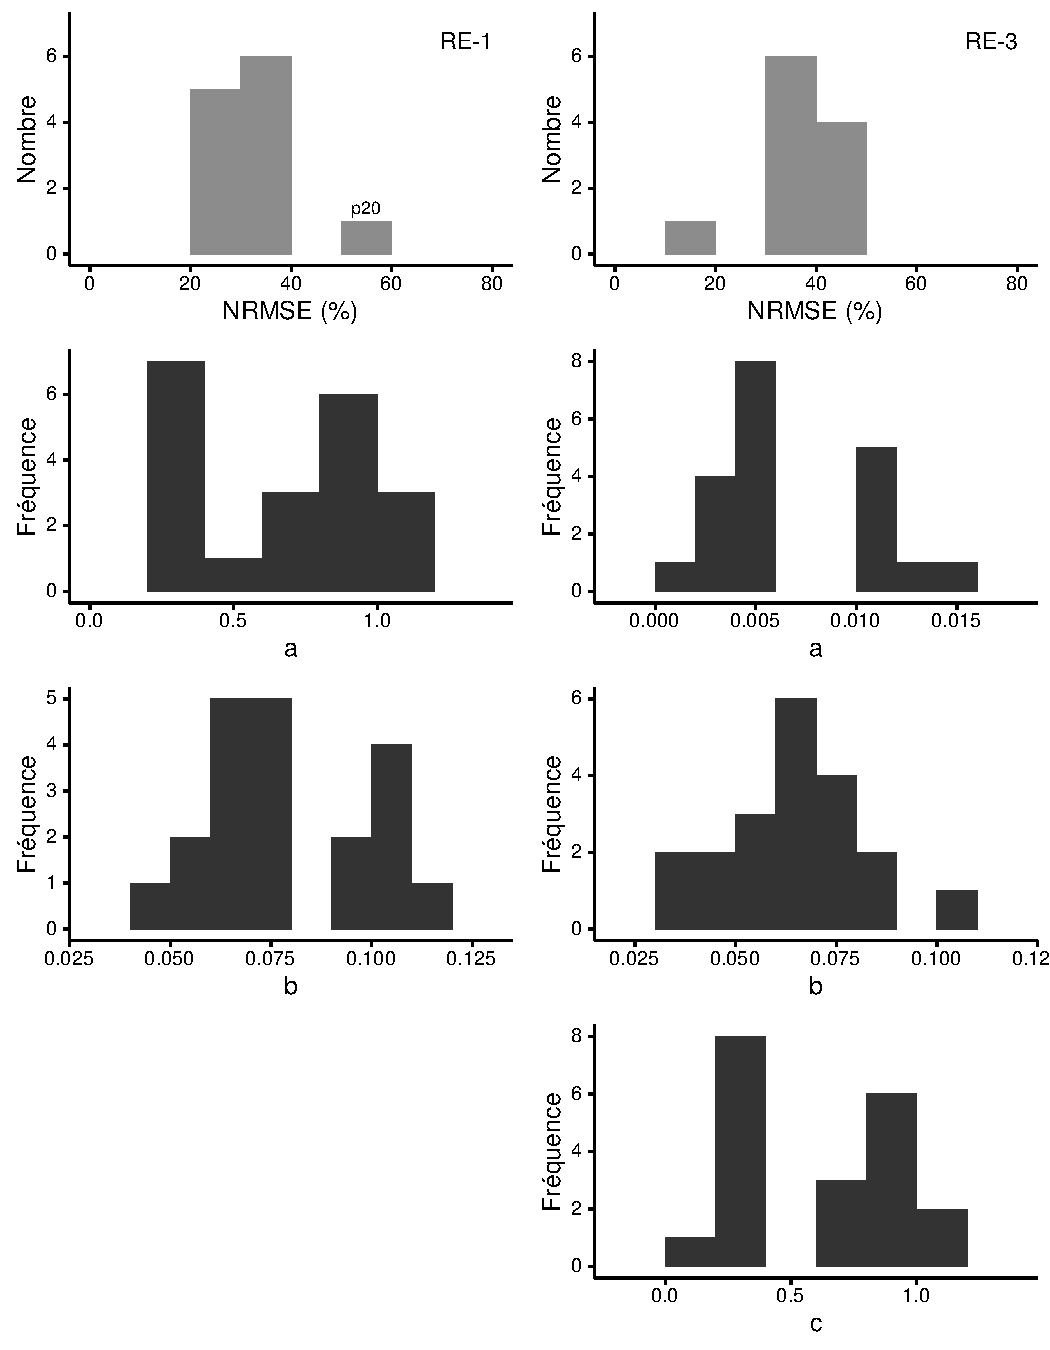
\includegraphics[width=.98\textwidth]{chap3/loc_ER}
\caption{Distribution de la NRMSE, du R\textsuperscript{2} (en gris) et des paramètres (en noir) des modèles RE-1 (à gauche) et RE-3 (à droite) calibrés par placette (N=20). Les lettres sous les graphes correspondent aux paramètres des équations utilisées.}
\label{fig:loc_ER}
\end{figure}

\begin{figure}
\centering
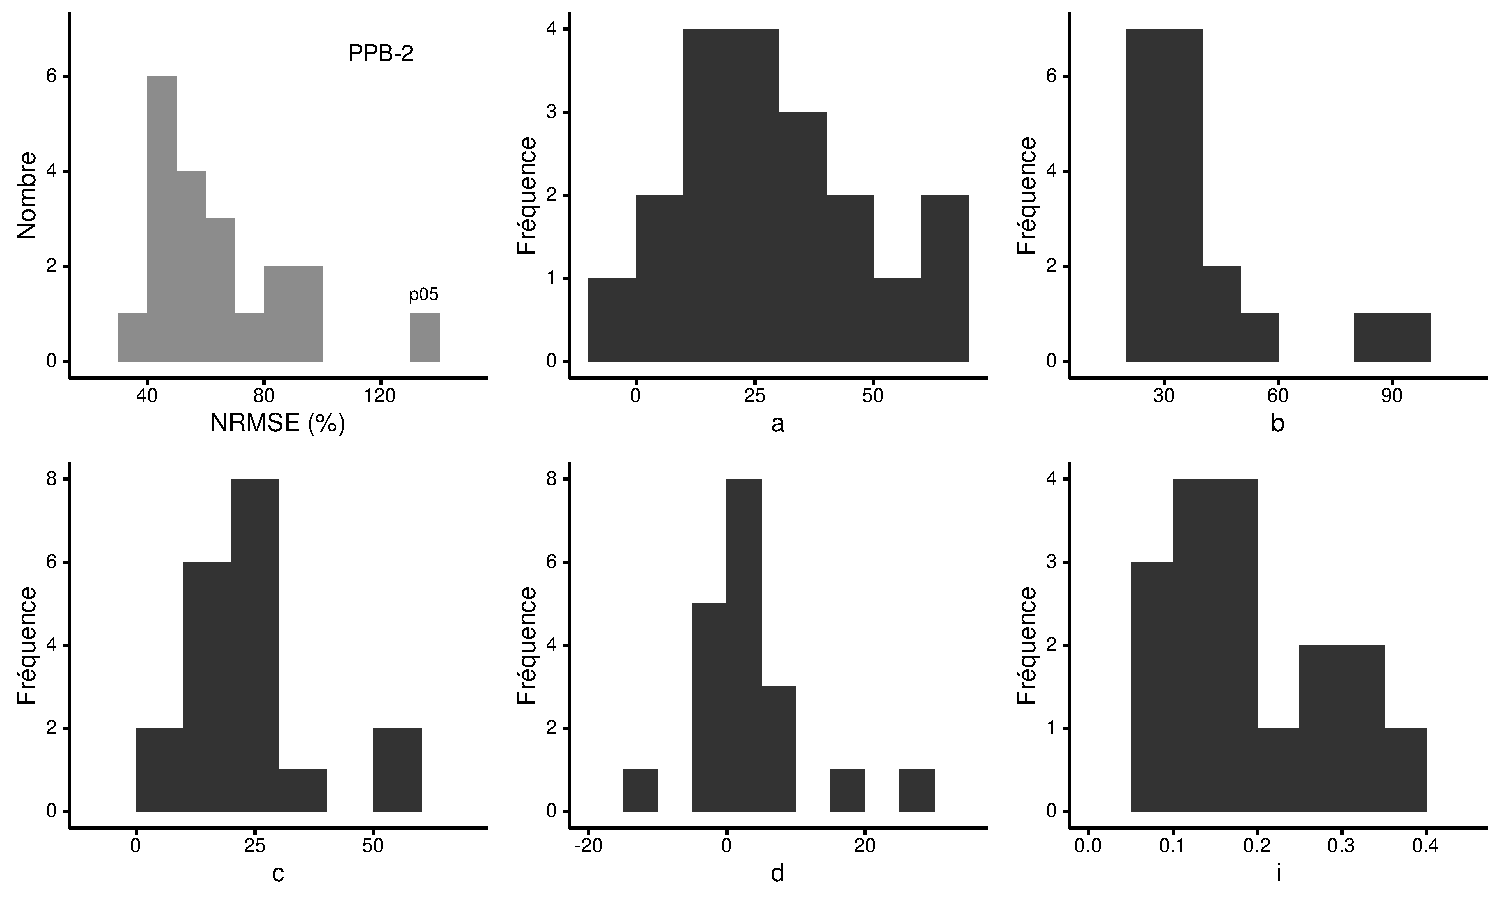
\includegraphics[width=1.15\textwidth, center]{chap3/loc_GPP}
\caption{Distribution de la NRMSE, du R\textsuperscript{2} (en gris) et des paramètres (en noir) du modèle PPB-2 calibré par placette (N=17). Les lettres sous les graphes correspondent aux paramètres des équations utilisées.}
\label{fig:loc_GPP}
\end{figure}

Les modèles RE-1, RE-3 ont pu être calibré pour l'ensemble des 20 placettes et le modèle PPB-2 pour 17 d'entre elles.
Le modèle RE-2, proche de RE-3 n'a pas été calibré.
Quant au modèle PPB-1, la calibration par placette ne convergeant pas pour la moitié d'entre elles, il n'a pas été pris en compte par la suite.
Il faut noter que la dispersion importante de points rend l'estimation des paramètres limitée en terme de significativité.
Par ailleurs que ce soit pour la PPB ou la RE, la placette n°10 semble avoir un comportement particulier.


Les R\textsuperscript{2} du modèle PPB-2, à l'exception de la placette n°10 , varient entre \num{0.5} et \num{0.9}.
La NRMSE se distribue entre 20 et \SI{60}{\percent}, ces valeurs sont supérieures à celles du modèle calibré à l'échelle de l'écosystème (\SI{19}{\percent}, Figure~ \ref{fig:ER_mdl_TairIVH}--d et \ref{fig:loc_GPP})).
Les paramètres du modèle PPB-2 varient de façon importante, entre \num{-6.1} et \num{66} pour a, entre \num{23.9} et \num{90.4} pour b, entre \num{6.2} et \num{60.0} pour c et \num{-10.7} et \num{27.1} pour d.

Toujours à l'exception de la placette n°10, pour les modèles RE-1 et RE-3 on constate une distribution des R\textsuperscript{2} au dessus de \num{0.5}, avec 11 placettes au dessus de \num{0.7} pour RE-1 et 15 pour RE-3.
Les valeurs de leurs NRMSE sont généralement plus élevées que celles obtenues à l'échelle de l'écosystème : entre 20 et \SI{55}{\percent} pour RE-1 (contre \SI{18}{\percent} à l'échelle de l'écosystème) et entre 15 et \SI{50}{\percent} pour RE-3 (contre \SI{13}{\percent}, Figure~\ref{fig:mdl_ER_Tair}--a, \ref{fig:ER_mdl_TairIVH}--d et \ref{fig:loc_ER}).
Les paramètres varient dans des gammes similaires pour RE-1 et RE-3 entre 0 et \num{1.1} pour a (RE-1) et a+c (RE-3) et entre \num{0.04} et \num{0.11} pour le paramètre b.


\begin{figure}
\centering
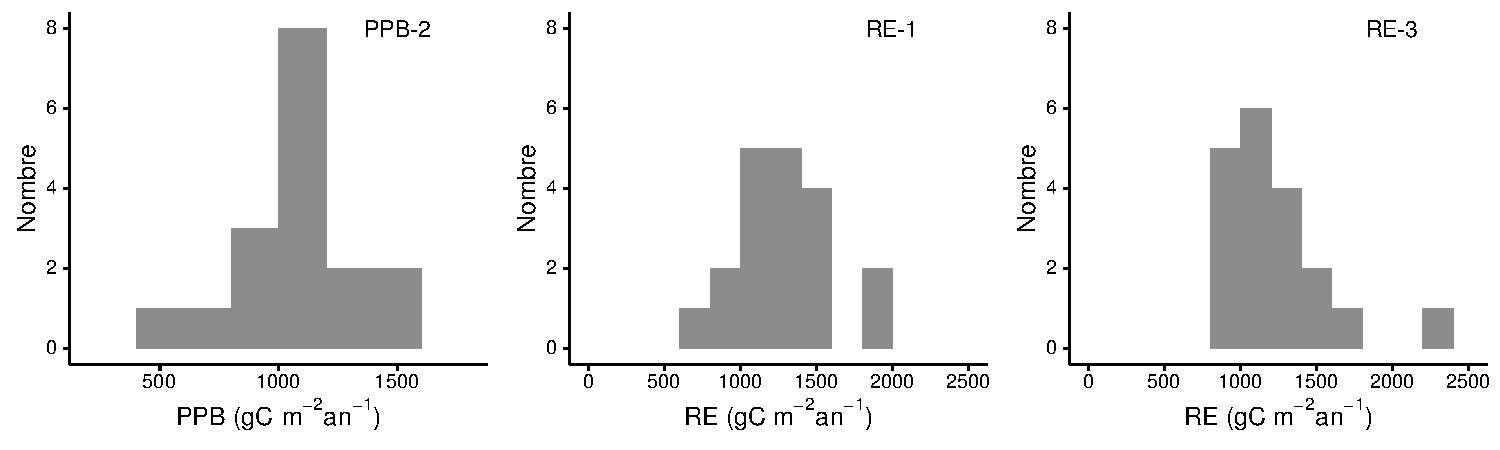
\includegraphics[width=1.15\textwidth, center]{chap3/distrib_flux_p7}
%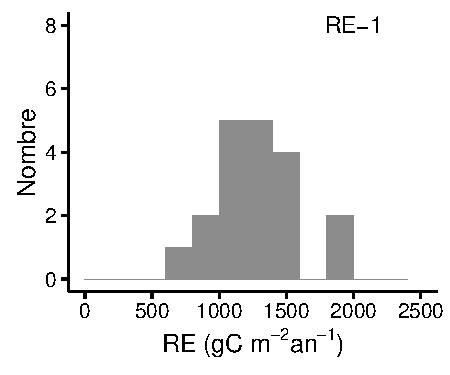
\includegraphics[width=.32\textwidth]{chap3/BdC_p7_RE1}
%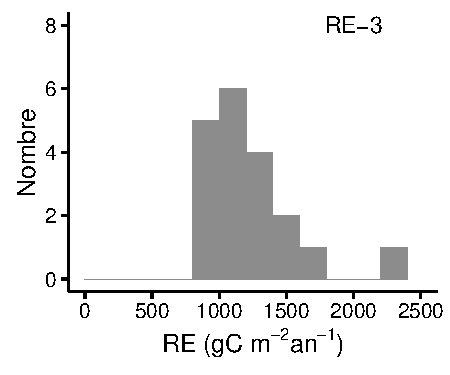
\includegraphics[width=.32\textwidth]{chap3/BdC_p7_RE3}
\caption{Distribution des flux estimés par placette en \si{gcma} pour le modèle PPB-2 (à gauche), RE-1 (au milieu) et RE-3 (à droite)}
\label{fig:distrib_fl_p7}
\end{figure}


Sur les deux années, les quantités de carbone assimilées par la PPB (modèle PPB-2) varient entre 507 et \SI{1409}{\gcma}, avec une majorité des placettes autour de \SI{1100}{\gcma} et une moyenne de \SI{1052(238)}{\gcma}.
Pour la RE, la distribution des flux du modèle RE-1 s'échelonne entre 633 et \SI{1832}{\gcma} avec une moyenne de \SI{1275(314)}{\gcma} et entre 828 et \SI{2371}{\gcma} avec une moyenne de \SI{1218(363)}{\gcma} pour le modèle RE-3.

Enfin il ne semble pas y avoir de gradient spatial des flux que ce soit pour la PPB ou la RE (Annexe~\ref{sec:carte_flux}).


%Que ce soit pour la RE ou la PPB , les gammes de paramètres sont larges mais cohérentes par rapport à celles obtenues à l'échelle de l'écosystème.



%Concernant la RE, les modèles RE-1 et RE-3 ont des valeurs de NRMSE relativement proche d'environ \SI{50}{\percent}, avec deux outliers pour RE-1 et un pour RE-3 (Figure~\ref{fig:loc_ER}).
%Les paramètres varient dans des gammes similaires pour les deux modèles.

%Concernant la PPB, le modèle PPB-2 a également une NRMSE importante, variant entre 40 et \SI{100}{\percent} avec un outlier.
%Les valeurs des paramètres varient également de façon importante (Figure~\ref{fig:loc_GPP}).

%\subsubsection{Corrélation avec facteurs contrôlant}

%\clearpage
\section{Discussion}

La discussion de ce chapitre, s'articule autour de quatre parties.
La première concerne les \textbf{modèles} calibrés à l'échelle de l'écosystème, leurs différences leurs qualités respectives.
La seconde détaille les différents \textbf{flux} estimés par ces modèles.
Le(s) \textbf{bilan(s)} de carbone issu(s) de ces flux sont exposés dans la troisième partie.
Enfin, la quatrième partie porte sur la \textbf{variabilité spatiale} des flux.

\subsection{Modèles à l'échelle de l'écosystème}

\subsubsection{PPB}

%\noindent
%\textit{Estimation de la PPB}

À l'inverse du modèle PPB-2, le modèle PPB-1 ne prend pas en compte de façon directe la végétation.
L'estimation des paramètres de PPB-1, lors de la phase de calibration, conduit à une incertitude forte : l'erreur standard est supérieure à \SI{60}{\percent} pour les paramètres $a$ et $b$ et à \SI{20}{\percent} pour les paramètres $c$ et $i$ (Tableau~\ref{table:mdl_par}).
Cette incertitude diminue pour PPB-2 avec l'intégration de l'IV, l'erreur est alors inférieure à \SI{20}{\percent} pour l'ensemble des paramètres.
Ces paramètres sont dans la gamme de ceux rapportés par \citet{june2004} : entre \num{23} et \SI{296.5}{\umle} pour la vitesse de transport des électrons photosynthétique à lumière saturante, entre \num{28.4} et \SI{55.7}{\degreeCelsius} pour la température optimale du transport et entre \num{13.9} et \SI{30.2}{\degreeCelsius} pour la différence de température à laquelle PPBsat vaut e\textsuperscript{-1}.
Lors de la phase de calibration, l'intégration de l'IV augmente la significativité des estimations et la représentativité des données mesurées.

Lors de l'évaluation et malgré une végétation similaire, l'augmentation de la NRMSE du modèle PPB-2, intégrant l'IV, est supérieure et dépasse (en valeur absolue) celle du modèle PPB-1. l'apport de l'IV dans l'estimation de la PPB n'est donc pas pertinent pour le jeu de données indépendant utilisé.
Par ailleurs, l'intégration de l'IV à un effet beaucoup plus important en 2013 (l'estimation du flux diminue de \SI{365}{\gcma}), qu'en 2014 (diminution de \SI{74}{\gcma}).
%
%La prise en compte de la végétation, si elle améliore les incertitudes statistiques sur l'estimation des paramètres du modèle, semblent conduire à une sous-estimation de la PPB.
%En effet le modèle PPB-2 ne rend pas compte des valeurs les plus élevées qui ont été mesurées (Figure~\ref{fig:BdC_GPP_interp}--B).
%Par ailleurs l'évaluation du modèle PPB-1 renvoie un erreur plus faible que celle du modèle PPB-2.

%
%Après interpolation la différence nette observée entre les modèles PPB-1 et PPB-2 est probablement liée à une sous-estimation des flux par ce dernier.

Les différences observées selon la façon d'estimer la PPB peuvent paraître importante, néanmoins elles sont du même ordre de grandeur que celle rencontré par \citet{worrall2009} qui compare différentes approches pour modéliser des flux de gaz avec des équations différentes.
%Ces différences sont également liées à la valeur élevée des flux qui font que, surtout dans le cas de modèles exponentiels, de faibles variations peuvent avoir des effets importants comme en témoigne l'analyse de sensibilité des paramètres du modèle (Tableau~\ref{table:mdl_sensitiv_BdC}).

L'intégration de la végétation aux modèles d'estimation de la PPB est rarement réalisé \citep{bortoluzzi2006a,gorres2014}, probablement à cause de la difficulté à prendre en compte ce signal.
La diversité des espèces végétales rend difficile la mise en place de protocole de suivi non-destructif généralisable à un grand nombre d'espèces.

Il semble que le modèle PPB-2 soit le plus pertinent pour estimer la PPB sur la tourbière de La Guette.

% % Apport IV
%Le modèle PPB-1 a une incertitude importante sur l'estimation de ses paramètres.
%L'apport de l'indice de végétation dans l'estimation de la PPB est important lors de la phase de calibration.
%Il permet de diminuer l'incertitude sur les paramètres du modèles, d'augmenter leur significativité et d'améliorer la représentativité des données mesurées.
%
%Malgré cette amélioration lors de la calibration, lorsqu'il est évalué sur un jeu de données indépendant, le modèle PPB-2 à une erreur standard plus importante que celle du modèle PPB-1.
%De plus après interpolation le modèle PPB-2 ne semble pas pouvoir représenter les valeurs maximum de PPB mesurée.
%L'apport de cet indice dans l'estimation de la PPB n'est donc pas généralisable.
%Bien que rarement faite à cause de la rareté des données, l'évaluation des modèles est cependant d'un intérêt fort afin de confirmer ou d'infirmer l'apport de l'ajout d'un prédicteur à un modèle, particulièrement si l'on souhaite l'extrapoler.

%% différences entre les modèles

%% Discuter la différence 2013-2014 ?
%\textbf{Discussion 2013-2014 ?}

%\noindent
%\textit{Estimation de la RE}
\subsubsection{RE}

À l'inverse de la PPB, l'intégration de la végétation pour modéliser la RE améliore peu l'estimation de la RE lors de la phase de calibration : la différence entre les valeurs de la NRMSE est de \SI{5}{\percent} (Figures~\ref{fig:mdl_ER_Tair}--a et \ref{fig:ER_mdl_TairIVH}--a,d).
En revanche lors de la phase d'évaluation, l'utilisation du recouvrement des herbacées améliore l'estimation de façon plus importante avec une différence de \SI{11}{\percent} entre les valeurs de NRMSE.
La différence apportée par l'intégration de la végétation (RE-2 ou RE-3) est du même ordre de grandeur en 2013 et en 2014.
Sur les 2 années, l'effet de l'intégration de la végétation est limité avec une différence de \SI{25}{\gcma} au maximum (entre RE-1 et RE-3), soit moins de \SI{2}{\percent} du flux.
%Encore une fois l'intérêt de l'évaluation est mis en avant puisqu'il permet de distinguer des modèles très proche lors de la calibration.
L'intérêt de l'évaluation pour la RE ne réside pas tant dans la sélection d'une meilleure estimation des flux.
Elle permet plutôt d'établir s'il est possible d'utiliser ou non un modèle dans un autre contexte.
%Pour la RE et le modèle RE-3 ce contexte reste contraint à l'intérieur du site.
Ainsi on peut envisager d'utiliser le modèle RE-3 sur d'autres données issues du même site.

% % Incertitude
Les incertitudes sur l'estimation des paramètres RE sont beaucoup moins importante que celle de la PPB.
L'estimation des paramètres des modèles, à l'exception du paramètre c du modèle RE-2, ont une p-value inférieure à 0,05 (Tableau~\ref{table:mdl_par}).
La NRMSE calculée lors de l'évaluation de ces modèles est certes plus importante que celle issue de la calibration, mais elle reste faible.
Ceci est particulièrement vrai pour le modèle RE-3 ou elle vaut moins de \SI{25}{\percent} (Figure~\ref{fig:ER_mdl_TairIVH}--f).
La RE semble donc mieux contrainte que la PPB, avec une estimation des paramètres plus fiable et une différence entre les estimations issues des différents modèles plus faible.

Le modèle RE-3 semble être le plus pertinent pour estimer la RE sur la tourbière de La Guette

\subsubsection{\fchh}
%\noindent
%\textit{Estimation du \fchh}
La calibration des flux de \chh conduit à une erreur du même ordre de grandeur que celle obtenue pour PPB-1 (Figure~\ref{fig:CH4_mdl}). 
L'évaluation du modèle fait doubler la NRMSE et montre sa limite : son utilisation est nécessairement restreinte à cette étude particulière.


\subsection{Les flux annuels à l'échelle de la tourbière de La Guette}

\subsubsection{Représentativité à l'échelle globlale}
%\noindent
%\textit{La production primaire brute}

\begin{figure}
\centering
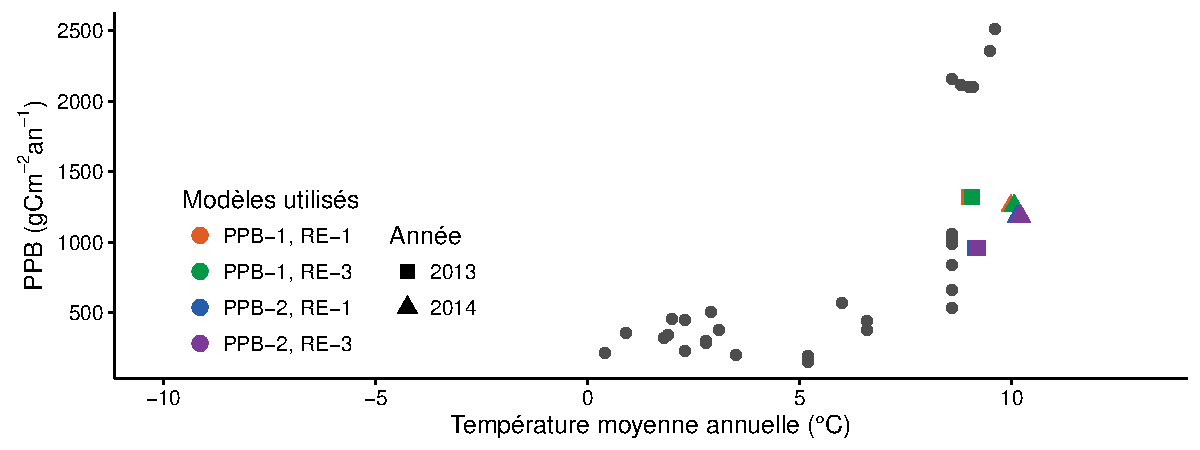
\includegraphics[width=\textwidth]{chap3/bib_vs_ppb}
\caption{Relation entre la production primaire brute (PPB) et la température moyenne annuelle (en °C) dans la littérature (points gris) et pour la tourbière de La Guette. Les couleurs correspondent aux différentes combinaisons de modèles utilisées.}
\label{fig:bib_vs_ppb}
\end{figure}

L'estimation des flux de \textbf{PPB}, est comprise entre 957 et \SI{1322}{\gcma} selon l'année et le modèle utilisé.
Ces valeurs sont élevées, en comparaison avec la PPB estimée par  \citet{trudeau2014} ou \citet{peichl2014} dans des tourbières boréales.
Elles sont respectivement comprises  123 et \SI{131}{\gcma} et entre 203 et \SI{503}{\gcma}.
C'est d'ailleurs dans ces gammes de valeurs, inférieures à celles relevées sur la tourbière de La Guette, que sont comprises la majorité des estimations (Figure~\ref{fig:bib_vs_ppb}).

%Pour le modèle PPB-1 l'année 2013 a une PPB plus forte que 2014, cependant les incertitudes sont telles que la comparaison n'a pas grand sens.
%Pour les estimations faites avec PPB-2, l'incertitude est moins important mais reste forte, et montre l'inverse : une PPB supérieure 2014 qu'en 2013.
%Cette observation serait davantage cohérente avec les valeurs de l'IV, légèrement plus haute en 2014 (Figure~\ref{fig:veg_evol}).

Une première hypothèse permettant d'expliquer cet écart, est la différence entre les températures moyennes sur les sites :
\SI{-4.3}{\degreeCelsius} et \SI{1.2}{\degreeCelsius} pour \citet{trudeau2014} et \citet{peichl2014} respectivement.
Ces températures sont bien plus faibles pour ces sites que sur la tourbière de La Guette.
Il semble que la PPB soit systématiquement inférieure à \SI{500}{\gcma} quand les températures moyennes annuelles ne dépassent pas \SI{5}{\degreeCelsius}. 
Au delà la gamme des flux est beaucoup plus large (Figure~\ref{fig:bib_vs_ppb}).
Ainsi d'autres études faite à des latitudes plus basse et des températures moyennes annuelles plus forte, montrent des estimation de la PPB plus proche de celles estimées sur la tourbière de La Guette.
Entre 534 et \SI{1058}{\gcma} par exemple pour \citet{beyer2015}, sur un site dont la température moyenne annuelle est de \SI{8.6}{\degreeCelsius} et avec une végétation proche de celle observée sur la tourbière de La Guette (\textit{Molinia caerulea}, \textit{Eriophorum augustifolium}, \textit{Sphagnum} spp).

Une part de l'explication de l'intensité de la PPB observée peut d'ailleurs être liée à la composition végétale du site.
Ainsi, \citet{jacobs2007} pour des prairies tourbeuses hollandaises, estiment des valeurs de PPB comprises entre 400 et \SI{2000}{\gcma} avec une moyenne de \SI{1300}{\gcma}.
Sur des écosystèmes similaires, au Danemark, \citet{gorres2014} trouvent des valeurs de PPB plus importantes encore, entre 1555 et \SI{2590}{\gcma}, mais avec des niveaux de nappe d'eau plus faibles (< \SI{-30}{\centi\metre}).
La tourbière de La Guette est envahie par une végétation vasculaire, notamment herbacée.
La comparer à des prairies tourbeuses est donc pertinent.
Dans ces deux cas les valeurs de PPB observées sont plus élevées que celles de la tourbière de La Guette.

%\noindent
%\textit{La respiration de l'écosystème}
%\subsubsection{La RE}

\begin{figure}
\centering
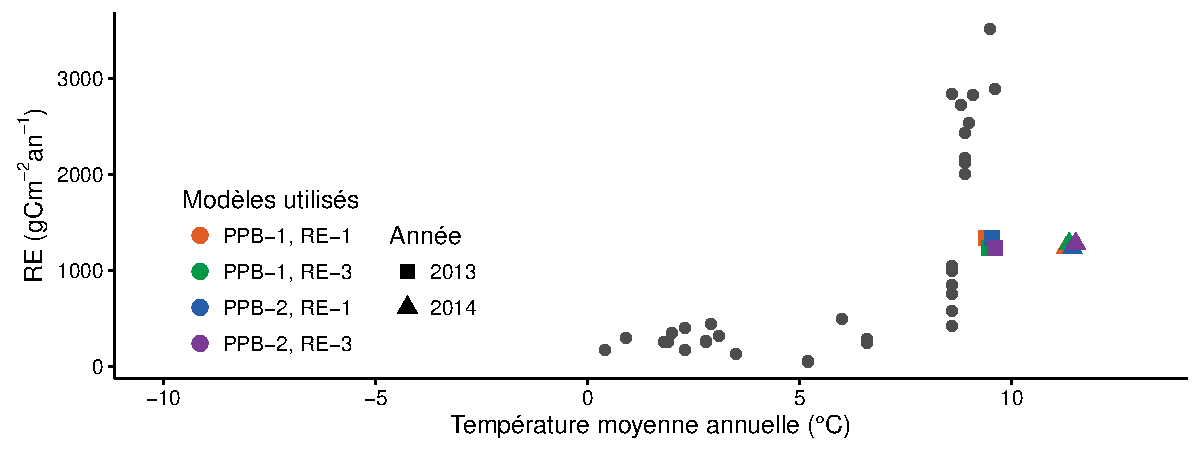
\includegraphics[width=\textwidth]{chap3/bib_vs_re}
\caption{Relation entre la respiration de l'écosystème (RE) et la température moyenne annuelle (en °C) dans la littérature (points gris) et pour ces travaux. Les couleurs correspondent aux différentes combinaisons de modèles utilisées.}
\label{fig:bib_vs_re}
\end{figure}

Les observations sur l'intensité des flux de la PPB sont également valables pour la respiration : la \textbf{RE} estimée sur la tourbière de La Guette est plus élevée que celles mesurées sur les tourbières boréales et plus faible que celles mesurées sur des prairies tourbeuses.
La RE estimée sur la tourbière de La Guette est comprise entre 1232 et \SI{1337}{\gcma} selon l'année et le modèle considéré (Figure~\ref{fig:bib_vs_re}).
Les estimations de la RE sont très proches pour les deux années, ce qui est cohérent avec le niveau de nappe d'eau relativement similaire également observé.
La différence de température de l'air entre 2013 et 2014 (\num{9.1} et \SI{10.1}{\degreeCelsius} respectivement) n'est pas suffisante pour observer une différence significative.

La comparaison de ces valeurs à celles des études citées précédemment, pour la PPB, montre qu'elles sont plus importantes que celles mesurées par \citet{peichl2014} et \citet{trudeau2014} (137 à \SI{443}{\gcma} et 206 à \SI{234}{\gcma} respectivement).
Elles s'approchent également des valeurs mesurées par \citet{beyer2015} (585 à \SI{1052}{\gcma}) et sont plus faibles que celles mesurées par \citet{jacobs2007} ou \citet{gorres2014} (500 à \SI{2000}{\gcma} et 2070 et \SI{3500}{\gcma} respectivement).
Comme pour la PPB, la température moyenne annuelle et la composition végétale des sites sont des explications possibles à ces observations.

%De la même façon que pour la PPB, les flux de la RE sont important si on les compare à des tourbières boréales et s'approchent davantage des flux mesurés dans les prairies sur sols tourbeux.
%La Re sur la tourbière de La Guette, comprise entre 1232 et \SI{1337}{\gcma} est plus importante que celle observée par \citet{peichl2014,trudeau2014} (pour reprendre les études citées précédemment) qui s'établissent respectivement entre 137 et \SI{443}{\gcma} et 206 et \SI{234}{\gcma}.
%Elles sont en revanche plus faible que celle mesurées par \citep{jacobs2007}, entre 500 et \SI{2000}{\gcma}, ou par \citep{gorres2014} : entre 2070 et \SI{3500}{\gcma}. 

De façon générale, les flux estimés sur la tourbière de La Guette sont cohérent avec les estimations relevées dans la littérature.


\subsubsection{Représentativité locale des flux de \coo}

Si l'on excepte la placette n°5, les modèles de la RE calibrés à l'échelle de l'écosystème permettent de représenter les placettes avec une NRMSE plus faible pour RE-3 par rapport à RE-1 : les pics des distributions sont autour de 40 et \SI{55}{\percent} respectivement (Figure~\ref{fig:repr_loc}).
Ces observations permettent de soutenir l'intérêt d'inclure l'indice de végétation dans la modélisation de la RE.

Pour la PPB (et toujours en excluant la placette n°5) la différence entre les deux modèles est moins forte (Figure~\ref{fig:repr_loc}).
La majorité des placettes ayant une NRMSE d'environ \SI{50}{\percent} pour les deux modèles, avec autant (7) de placettes ayant une NRMSE inférieure à \SI{50}{\percent} que de placette (13) ayant une NRMSE supérieure.
Il ne semble par y avoir de différences significatives dans la représentativité locale des modèles PPB-1 et PPB-2.




%\noindent
%\textit{Le flux de \chh}
\subsubsection{\fchh}

\begin{figure}
\centering
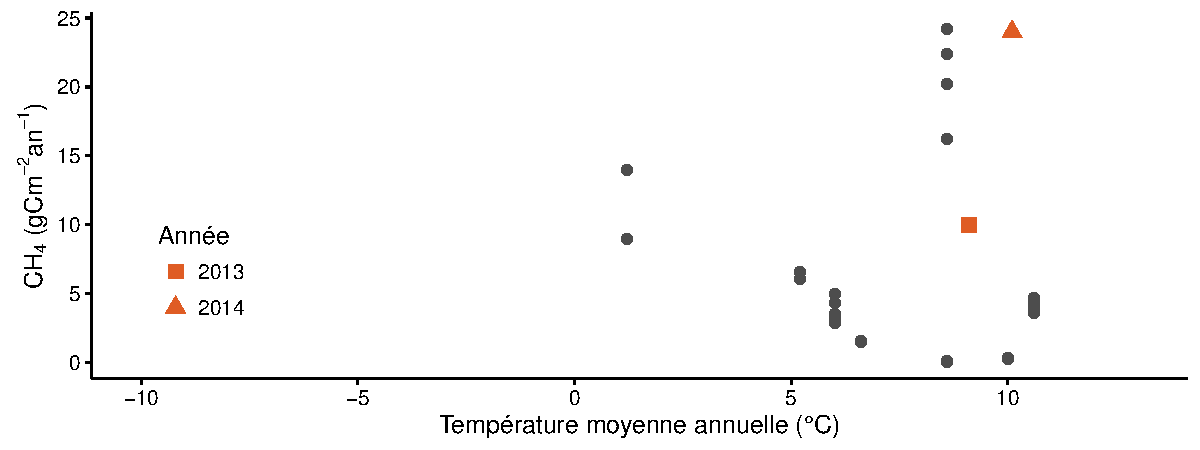
\includegraphics[width=\textwidth]{chap3/bib_vs_ch4}
\caption{Relation entre les flux de \chh  et la température moyenne annuelle (en °C) dans la littérature (points gris) et pour ces travaux (en rouge).}
\label{fig:bib_vs_ch4}
\end{figure}

Comparés aux flux de \coo, les flux de \chh mesurés sur la tourbière de La Guette sont faibles : deux ordres de grandeur inférieurs.
Ces flux sont dans la gamme des valeurs présentes dans la littérature, de 1 à \SI{40}{\gcma} (Figure~\ref{fig:bib_vs_ch4},  \citep{nilsson2001}).
Pour 2013 les valeurs mesurées sont proches de celles mesurées par \citet{nilsson2008} (entre 9 et \SI{14}{\gcma}).
%Plus généralement, \citet{nilsson2001} estiment les émissions des tourbières suèdoises entre 1,5 et \SI{40}{\gcma}.
L'absence d'étiage en 2014 expliquerait le doublement des flux en minimisant la zone aérobie et les possibilités d'oxydation du \chh \citep{lai2009}.
Les faibles variations du niveau de nappe sont probablement à l'origine de l'absence de relation entre ce dernier et les flux de \chh.
Ces observations corroborent les observations faites par \citet{trudeau2012} et \textbf{(à developper, de ref ds trudeau2012)}


%\noindent
%\textit{Le carbone organique dissout}
\subsubsection{Le COD}

L'intensité des flux de COD estimés sur la tourbière de La Guette sont très faibles comparés aux flux de \coo.
Par ailleurs, ils sont du même ordre de grandeur que les flux de \chh.
Les quantité de COD exportées par la tourbière sont dans la gamme de celles présentes dans la littérature.
Elles sont plus faibles que celles estimées par \citet{worrall2009} (entre 10 et \SI{86}{\gcma}), mais plus importantes que celles estimées par \citet{carroll1997} dans une tourbière de bas-marais d’Amérique du nord (\SI{3.4}{\gcma}) ou celles rapportées par \citet{waddington2000} (<\SI{6}{\gcma}) dans une tourbière de haut-marais suédoise.

Le doublement du flux de COD observé en 2014 par rapport à 2013 est lié à une quantité plus importante d'eau quittant la tourbière et présentant des concentrations en COD similaires (Figure~\ref{fig:discharge}).
Dans le même temps le niveau de nappe moyen mesuré en 2014 est légèrement supérieur à celui mesuré en 2013 et les précipitations sont du même ordre de grandeur (Figure~\ref{fig:WTL} et \ref{fig:pluvio}).
Ces observations permettent de faire l'hypothèse que l'année 2013 a permis à la tourbière de reconstituer une partie de son stock d'eau perdu lors des années précédentes plus sèches.



\subsubsection{Incertitudes et limitations du bilan}
Les incertitudes les plus fortes du bilan sont sur les flux de \chh avec une NRMSE de \SI{32}{\percent} lors de la calibration et de \SI{68}{\percent} lors de la validation.
Cette différence importante montre que l'estimation des flux de \chh à l'aide de l'indice de végétation à permis l'estimation de sa contribution au bilan de carbone de l'écosystème pour les années 2013 et 2014, mais que son utilisation dans d'autres conditions (année sèche, température moyenne annuelle significativement différente) est limitée.
L'importance faible du \chh dans le bilan de carbone de la tourbière rend ces incertitudes moins critiques que celles faite sur l'estimation de la PPB.
Les incertitudes importantes sur la PPB, sont mises en évidence par les fortes variations des flux interpolés selon l'équation utilisée.
Elles sont la source des variations observées en termes de bilan.
%L'ajout d'un indice de végétation diminue d'incertitude des paramètres du modèle, mais cet apport n'est pas reflété par l'évaluation, malgré la similarité de la végétation.
À l'inverse la RE est bien contrainte.
Sur les 2 années la différence entre les différentes équations utilisées ne dépassent pas \SI{25}{\gcma}.

En outre le bilan de carbone est aussi limité par sa représentativité. 
Différents éléments n'ont pas été pris en compte dans les mesures et l'établissement du bilan.
La strate arborée notamment, largement présente dans certaines zones, n'est pas considérée directement.
Les zones, restreintes, de touradons également, de même que les arbustes dépassant la taille de la chambre ou encore les zones d'eau libre.
%Ainsi la strate arborée fortement présente dans certaines zones n'est pas directement prise en compte.
%De la même manière une partie restreinte de la tourbière mais néanmoins présente est constitué de touradons dont l'effet n'a pas été pris en compte. %\plop (\textbf{biblio effet microtype}).

\subsection{Estimations du bilan net de l'écosystème à l'échelle de la tourbière de La Guette}

\begin{figure}
\centering
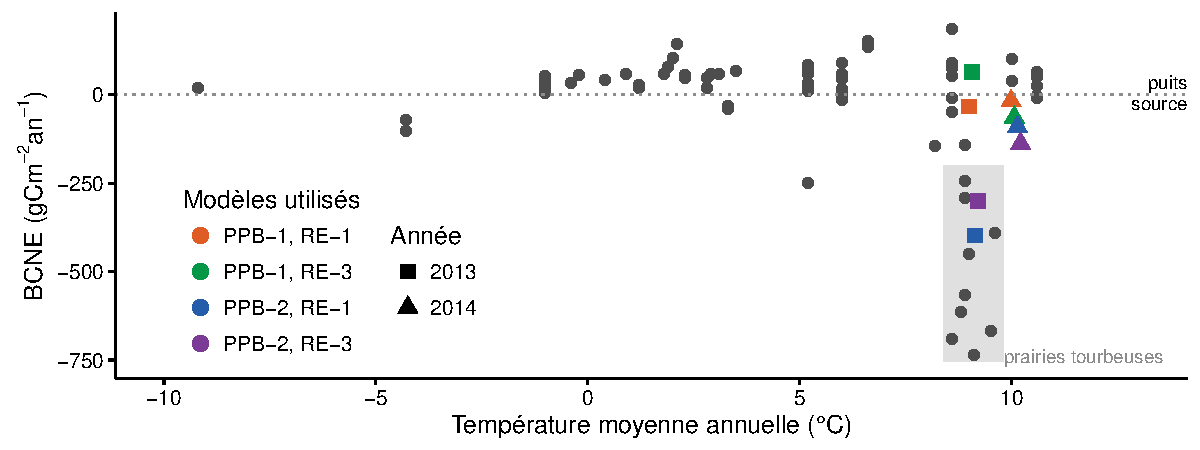
\includegraphics[width=\textwidth]{chap3/bib_vs_necb}
\caption{Relation entre le bilan de carbone net de l'écosystème (BCNE) et la température moyenne annuelle (en °C) dans la littérature (points gris) et pour ces travaux.  Les couleurs correspondent aux différentes combinaisons de modèles utilisées et la ligne de tirets sépare les écosystèmes stockant du carbone (au dessus) de ceux libérant du carbone (en dessous).}
\label{fig:bib_vs_necb}
\end{figure}

\subsubsection{Puits ou source ?}

En considérant les estimations qui semblent les plus pertinentes pour la PPB (PPB-2) et pour la RE (RE-3), on peut dire la tourbière de La Guette est une source de carbone.
Ainsi elle émet, en moyenne sur les deux années, environ \SI{220(33)}{\gcma} (Tableau~\ref{table:bdc}).
%Les quantités de carbone émises dans l'atmosphère sont comprises entre 0 et \SI{245}{\gcma} (Tableau~\ref{table:bdc}).
%Ces différences sont principalement liées à l'estimation de la PPB.
%Les bilans calculés à l'aide du modèle PPB-2 estiment une source de carbone supérieure à \SI{200}{\gcma}.
%Selon le bilan considéré, la tourbière de La Guette stocke de faible quantité de C de l'ordre d'une dizaine de grammes par mètre carré, ou émet du carbone dans l'atmosphère de l'ordre de \num{14} à de \SI{233}{\gcma}.
Ces valeurs, sont du même ordre de grandeur que celles mesurées dans des prairies tourbeuses (Figure~\ref{fig:bib_vs_necb}).
%Elles restent cependant sujettes à caution car il est possible que le modèle PPB-2 sous-estime la PPB et donc sur-estime les pertes de carbone par la tourbière (Figure~\ref{fig:BdC_GPP_interp}).
La tourbière est également une source de carbone plus importante en 2013 (\SI{-301(47)}{\gcma}) qu'en 2014 (\SI{-138(20)}{\gcma}).
La légère baisse du niveau de la nappe d'eau en 2013 ne se traduit pas par une RE plus importante et cette différence est principalement liée à une hausse de la PPB.
Cette hausse de la PPB est peut être liée à l'histoire du site : les années précédant les mesures sont sèches est ont pu amoindrir le potentiel de photosynthèse de l'écosystème, notamment de ses plantes pérennes (mousses et arbustes).
Ce potentiel en cours de rétablissement pendant le suivi serait donc plus fort en 2014.
%Par contre le fait que les estimations qui utilisent PPB-2 montrent une source de carbone plus importante en 2013 qu'en 2014 semble cohérent.
%En effet le peu de baisse du niveau de la nappe d'eau mesuré pendant les deux années de mesure a eu lieu en 2013.
Elles se rapprochent de celles mesurées dans des tourbières de bas-marais d'Amérique du nord : \SI{-145}{\gcma} \citep{carroll1997} ou celles mesurées dans une autre tourbière de bas-marais en Allemagne (\num{-142} à \SI{-565}{\gcma}) mais utilisée comme prairie permanente \citep{beyer2015}.

%Les estimations utilisant PPB-1 semblent indiquer que la tourbière est une légère source de carbone ou s'approche d'un équilibre.
%Avec ces estimations les bilans 2013 et 2014 sont beaucoup plus proches et la PPB est légèrement plus forte en 2013 qu'en 2014.
%Même se cette observation semblent aller à l'inverse des observations de terrain (un IV plus fort en 2014) les incertitudes sont telles qu'il est difficile d'écarter les estimations utilisant PPB-1 sur ce seul aspect.
%Ce constat est également cohérent avec les observations de terrain, qui montre un niveau de nappe particulièrement élevé pendant les deux années de mesure en comparaison avec les précédentes.

%Pour résumer, il est probable que la tourbière de La Guette a plutôt fonctionner comme une source en moyenne sur les deux années.
%Elle a probablement été une source plus importante en 2013 qu'en 2014 avec cependant des émissions de carbone probablement un peu moins importante que celles prédites en utilisant PPB-2.



%Les bilans annuels ont des comportements différents en 2013 et en 2014.
%En 2013 l'écart entre les deux estimations les plus extrêmes est de \SI{462}{\gcm}.
%Cet écart est lié principalement à la prise en compte de la végétation (utilisation de PPB-2 au lieu de PPB-1).
%En comparaison l'écart observé entre estimations extrêmes est quatre fois plus faible en 2014 (\SI{120}{\gcm}).


\subsubsection{Importance relative des flux}

D'une manière générale, les bilans sont principalement fonction de l'intensité des flux de \coo.
Le \chh et le COD ont une place marginale en termes de quantité de carbone.
Ces observations sont cohérentes avec d'autres études comme \citet{bortoluzzi2006a,worrall2009}.
Cependant si le \chh ne semble pas jouer un rôle majeur sur le bilan de carbone de la tourbière de La Guette, il faut considérer le fait que seul le flux diffusif de \chh a pu être mesuré et estimé (c'est également le cas pour les études citées précédemment).
Les émissions de \chh par ébullition sont exclues du bilan.
Rarement estimé, ce flux peut représenter 17 à \SI{66}{\percent} d'une émission \citep{gogo2011,christensen2003}, et être potentiellement très fort : plus de \SI{35}{\gcm} par événement \citep{glaser2009}.
La présence de végétaux vasculaires qui en transportant le \chh dans l'atmosphère diminuent la concentration en \chh dans le sol tendraient cependant à diminuer ce phénomène \citep{chanton2005}.



\subsection{Variabilité spatiale sur la tourbière de La Guette}

\subsubsection{Distribution des groupes de végétation}


\begin{figure}
\centering
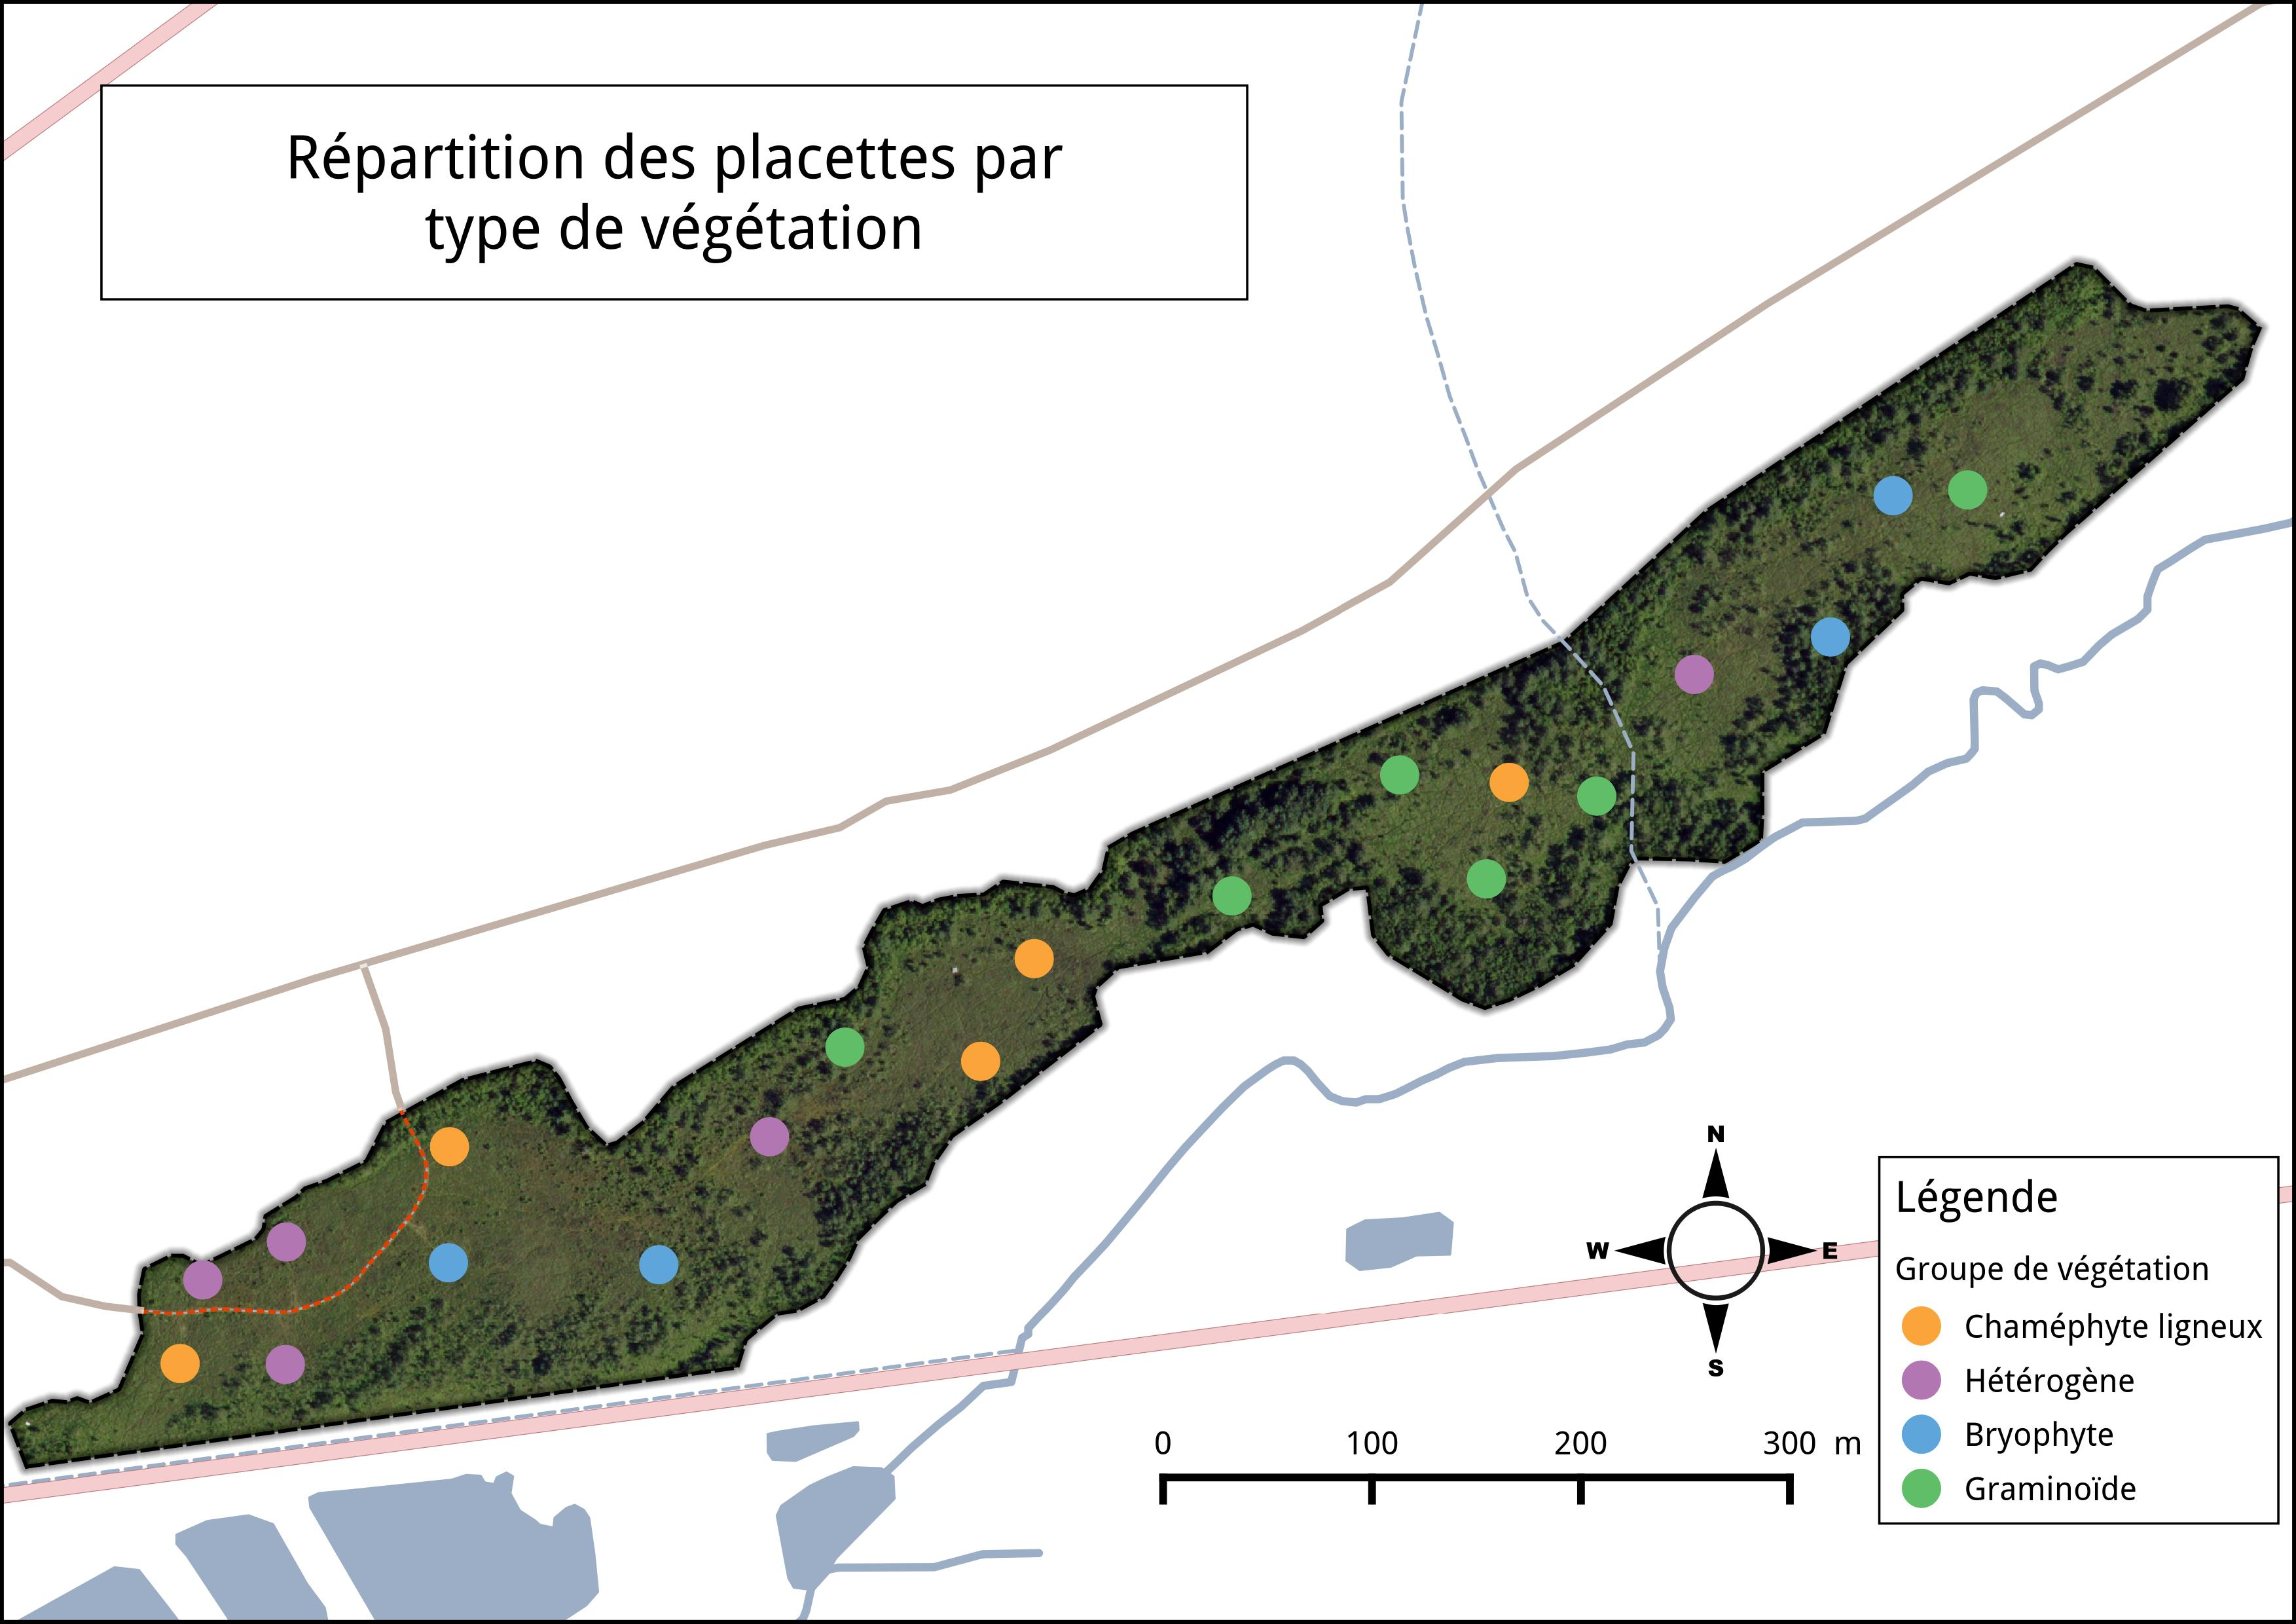
\includegraphics[width=.98\textwidth]{chap3/carte_grpveg}
\caption{Distribution des groupes de végétation sur la tourbière de La Guette.}
\label{fig:carte_grpveg}
\end{figure}

Si quelques placettes proche géographiquement ont des recouvrement végétaux voisins (les placettes p18 et p19 ; p02, p03 et p04 ; p12, p14 et p16) les autres ne présentent pas un tel lien (Figure~\ref{fig:carte_grpveg}).
Par ailleurs, au sein d'une même classe peuvent être rassemblées des placettes très éloignées spatialement, les placette p01 et p15 par exemple ou les placettes p02 et p17 ou p09 et p20.
Ceci montre une variabilité spatiale importante du recouvrement végétal mais également que cette variabilité ne semble pas répartie géographiquement, selon un gradient quelconque.

\subsubsection{Effet du type de végétation majoritaire sur les flux et le bilan de \coo}

L'estimation des flux par groupe de végétation montre que lorsque la strate muscinale est la plus importante, l'intensité des flux est plus faible.
Cette observation est valable pour la PPB, ce qui est cohérent avec le fait que le sphaignes sont connues pour avoir une production plus faible \citep{rydin2013b,beyer2015}, et elle est également valable pour la RE.
Dans ce cas le niveau élevé de la nappe d'eau et la proportion plus faible de plantes vasculaires, qui permettent l'aération du milieu et la stimulation de la RE par la libération d'exsudats racinaires, permet d'expliquer la faible intensité du flux.

Les groupes Mix et Arbustes sont proches et sont des sources de carbone importantes quelle que soit la combinaison de modèles.
La RE de ces groupes est plutôt élevée (> \SI{1200}{\gcma}), et est couplée à une PPB plutôt faible (située entre celle du groupe Mousse et celle du groupe Herbe).
Le point commun de ces deux groupes est la proportion de la strate arbustive qui dépasse \SI{50}{\percent}.
Ceci est cohérent avec la croissance limitée de la strate arbustive (par rapport à la strate herbacée) au cours de la saison de végétation (donc PPB plus faible) \citep{rydin2013b}.
La Re plus forte peut elle s'expliquer par la présence des racines.

Le groupe Herbe est le plus particulier, son comportement varie de façon importante en fonction des modèles.
C'est le seul groupe dont une estimation du bilan est positive (fonction puits) ce qui est contraire à ce que l'on attend.
En effet on attend avec l'envahissement du site par une végétation vasculaire une diminution de la fonction puits ou une augmentation de la fonction source liée à une augmentation de la RE.
Cette augmentation de la RE n'est pas visible, le groupe Herbe est même celui pour lequel la RE est la plus faible.
Pour expliquer cette observation on peut faire l'hypothèse que le potentiel de photosynthèse des plantes pérennes, notamment des sphaignes, n'ait pas encore retrouvé son maximum après avoir été affaibli pendant les années sèches précédents les mesures.
Cette hypothèse est cohérente avec une photosynthèse forte de la Molinie telle qu'on peut l'observer (Tableau~\ref{table:flux_grp}).
La PPB de la strate herbacée (principalement la Molinie) n'est pas ou peu limité que ce soit par l'histoire du site (c'est une plante annuelle) ou le niveau de la nappe.
En effet espèce de cette strate on la capacité d'échanger du gaz de leur racines à l'atmosphère grâce à l'aérenchyme, ce qui leur permet de se développer dans des milieux inondés \citep{taylor2001,rydin2013c}.
%Pour expliquer cette observation on peut faire l'hypothèse que le niveau de nappe élevé limite la respiration, notamment hétérotrophe, la respiration hétérotrophe étant moins limitée par la capacité de la strate herbacée à échanger du gaz de leur racines à l'atmosphère grâce à l'aérenchyme \citep{taylor2001,rydin2013c}.
%De la même manière la PPB ne serait pas ou peu limitée par le niveau de la nappe d'eau, ce qui est cohérent avec les observations de terrain montrant un développement de la Molinie aussi important en 2013 qu'en 2014.
%Le bilan du groupe Herbe s'expliquerait donc par le niveau élevé de la nappe d'eau limitant la respiration hétérotrophe tout en ne limitant pas, ou moins la PPB.
%Il n'est cependant par sure que sur le long terme cette situation perdure.

\subsubsection{Quantification de la variabilité spatiale}

La distribution des flux calculés par placette permet, de faire une première estimation quantifié de la variabilité spatiale.
La variabilité spatiale mesurée sur le site de La Guette est relativement forte comparée aux moyennes observées dans différents sites (Figure~\ref{fig:vs_bib}--A).
La variabilité spatiale de la RE, similaire en 2013 et 2014, l'est davantage encore (Figure~\ref{fig:vs_bib}--B).
La variabilité spatiale du bilan, dépasse les moyennes relevées dans la littérature (Figure~\ref{fig:vs_bib}--C).

Ces comparaisons sont évidemment à regarder avec précaution, l'erreur liée aux estimations faites par placettes étant forte.
Néanmoins ces graphes montrent l'importance de la variabilité spatiale des flux à l'échelle d'une tourbière et permettent de mettre cette variabilité en perspective par rapport aux moyennes usuellement rapportées.


\begin{figure}[!htb]
\centering
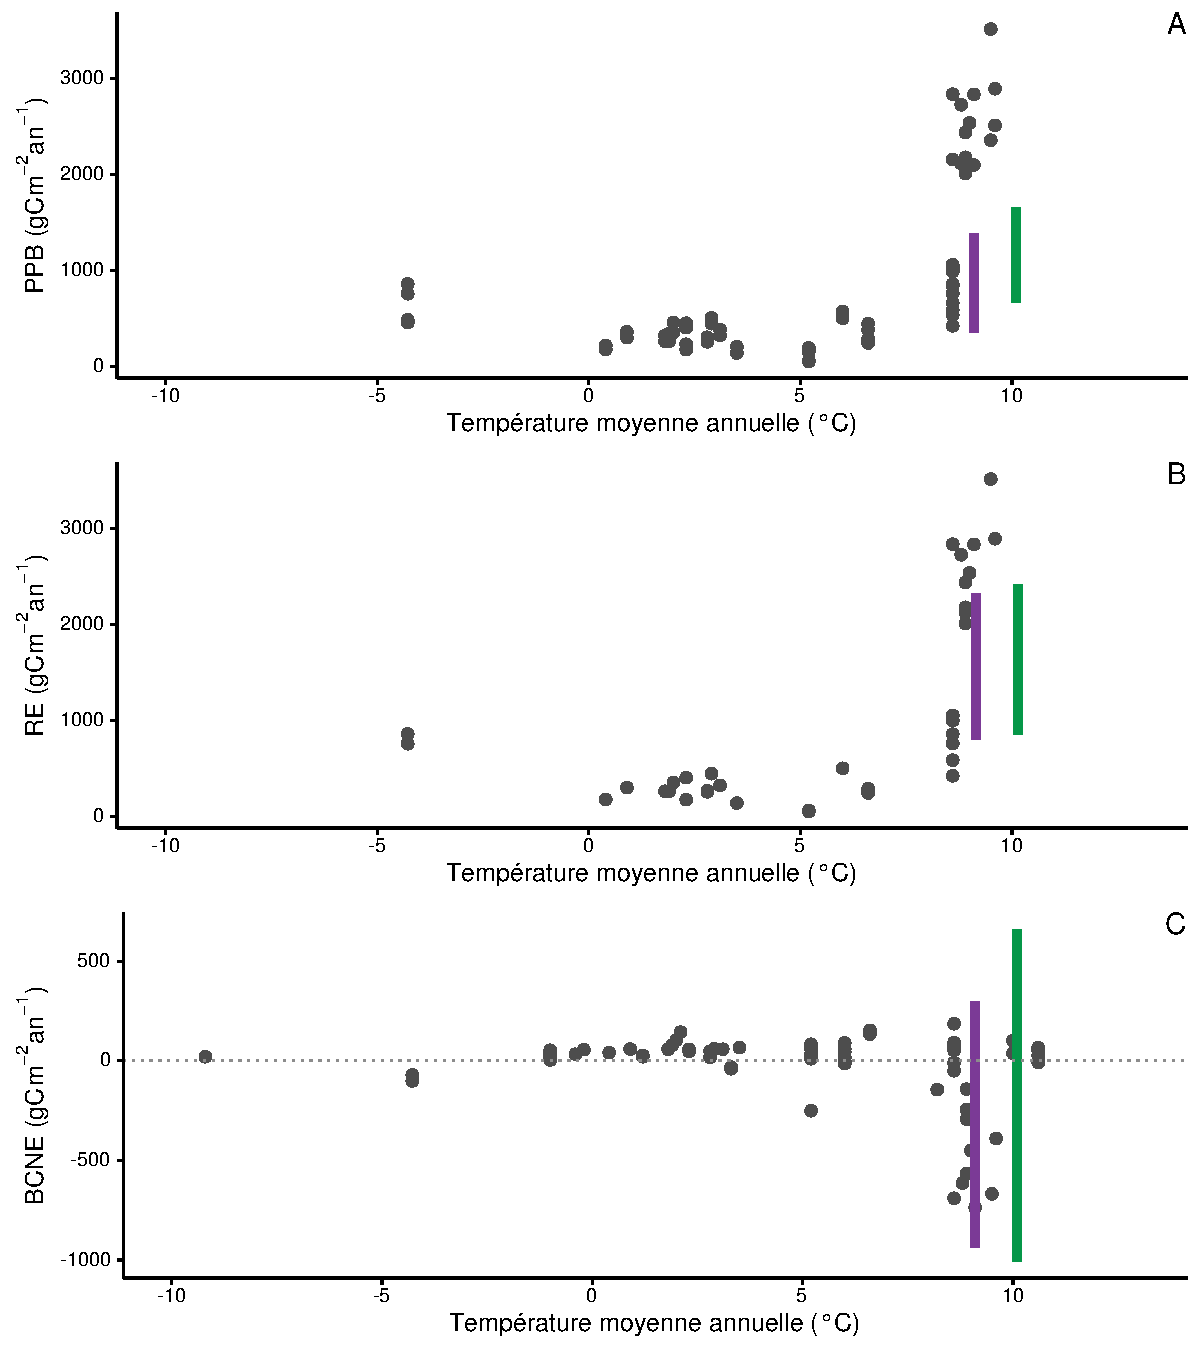
\includegraphics[width=.98\textwidth]{chap3/vs_bib}
\caption{Variabilité spatiale, par placette, des flux issus des modèles PPB-2 et RE-3, comparée aux valeurs relevées dans la littérature (points gris). Les barres violettes représentent les gammes mesurées en 2013 et les barres vertes celles mesurées en 2014. Le tableau de l'annexe~\ref{table:bibliodata} recense les références utilisées.}
\label{fig:vs_bib}
\end{figure}
%
%\begin{table}[!htb]
%\centering
%\caption{Variabilité temporelle (multi-annuelle) des flux de \coo dans les tourbières}
%\label{table:bib_var}
%\begin{tabular}{llllllll}\toprule
%& & \multicolumn{3}{c}{RE} &  \multicolumn{3}{c}{PPB} \\ \cmidrule(lr){3-5} \cmidrule(lr){6-8} 
%référence & période de mesure& min & max & $\frac{max}{min}$ & min & max & $\frac{max}{min}$\\ \midrule
%\citet{worrall2009}& 1993--2005 & 151 & 190 & 1,3 & 49 & 58 & 1,2 \\
%\citet{peichl2014} & 2001--2012 & 203 & 503 & 2,5 & 137 & 443 & 3,2 \\
%\bottomrule
%\end{tabular}
%\end{table}


%Le calcul des bilans avec les différents groupes de végétation permet de mettre en évidence des comportements différents des flux selon la végétation majoritaire.
%Ainsi le groupe 3 dans lequel la strate herbacée est la plus importante est celui ou la PPB est la plus forte.
%Ce point semble en cohérence avec la croissance annuelle importante des herbacées visible sur le terrain.
%Mais également car la présence d'un Aérenchyme permet à la molinie et à la linaigrette d'alimenter leurs racines en oxygène malgré un niveau de nappe très élevé \citep{taylor2001,rydin2003c}).
%À l'inverse le groupe 1 dans lequel la strate muscinale est la plus importante est également le groupe pour lequel la PPB est la plus faible.
%\plop
%
%Pour la RE, ce sont les groupes 3 et 4 qui ont les flux estimés les plus importants avec une différence d'environ \SI{200}{\gcma} avec les deux autres groupes.
%Malgré leurs différences, le groupe 2 possède une strate muscinale importante alors qu'elle est absente dans le groupe 3, ils ont en commun d'avoir une strate arbustive importante.

%\subsection{Représentativité locale du modèle}
%
%
%Si l'on excepte la placette n°5, les estimations de la RE à l'échelle de l'écosystème permettent de représenter les placettes avec une erreur comprise entre 20 et \SI{100}{\percent} pour RE-1 et entre 20 et \SI{80}{\percent} pour RE-3.
%La majorité des placettes à une erreur d'environ \SI{55}{\percent} pour RE-1 et d'environ \SI{40}{\percent} pour RE-3 (Figure~\ref{fig:repr_loc}, RE-1 et RE-3).
%Ces observations permettent de soutenir l'intérêt d'inclure l'indice de végétation dans la modélisation de la RE.
%Pour la PPB, toujours à l'exception de la placette n°5, les estimation à l'échelle de l'écosystème permettent de représenter les placettes avec une erreur comprise entre 20 et \SI{90}{\percent} pour PPB-1 et entre 30 et \SI{100}{\percent} pour PPB-2.
%La majorité des placettes ayant une erreur d'environ \SI{50}{\percent} pour les deux modèles, avant autant (7) de placettes ayant une erreur inférieure à \SI{50}{\percent} que de placette (13) ayant une erreur supérieure.

